% !TEX program = xelatex
\documentclass[12pt,a4paper,oneside]{book}
% !TEX root = ../do-an.tex
% =====================================================================
%  styles/settings.tex
%  Các thiết lập chung, nạp từ file chính do-an.tex.
%  SINH VIÊN KHÔNG SỬA FILE NÀY.
%
%  Lưu ý: lệnh khai báo lớp tài liệu nằm ở file do-an.tex chứ không nằm
%  ở đây. Lý do: Overleaf dò file chính bằng cách tìm chuỗi khai báo lớp
%  tài liệu trong các file. Nếu chuỗi đó xuất hiện ở file này, Overleaf
%  sẽ biên dịch nhầm file này và báo lỗi "no legal end found", vì file
%  này chỉ chứa thiết lập chứ không chứa phần thân tài liệu.
% =====================================================================

% Toàn bộ nhận diện DAU: phông, màu, bìa, hộp trình bày, header
\usepackage{styles/dau}
\dauLayout

% Giãn dòng và khoảng cách đoạn theo quy cách đồ án
\linespread{1.25}
\usepackage[skip=8pt plus 1pt, indent=15pt]{parskip}

% Ghi chú: mẫu gốc dùng gói atbegshi để vứt trang đầu, vì trang bìa của
% mẫu gốc dựng bằng minipage nên sinh ra một trang trắng. Trang bìa ở
% đây dựng bằng môi trường titlepage nên không có trang trắng, và nếu
% giữ thủ thuật đó thì chính trang bìa sẽ bị vứt mất.

\usepackage{longtable}
\usepackage{needspace}
\hypersetup{pdftitle={EduShield AI - He thong thi truc tuyen va ho tro giam sat},pdfauthor={Nhom thuc hien - can bo sung}}
\newcommand{\src}[1]{{\small\nolinkurl{#1}}}
\newcommand{\pending}[1]{\textcolor{daumaroon}{[#1]}}
\newcolumntype{L}[1]{>{\raggedright\arraybackslash}p{#1}}
\tikzset{reportbox/.style={draw=daunavy,rounded corners,fill=lightnavy,align=center,font=\small,text width=4.3cm,minimum height=1cm},reportarrow/.style={-{Stealth},thick,draw=daunavy}}
\setlength{\emergencystretch}{2em}
% Thông tin tác giả theo hồ sơ báo cáo gốc.
\crname{BÁO CÁO ĐỒ ÁN TRÍ TUỆ NHÂN TẠO}
\cmonhoc{Học phần AIP202 \textperiodcentered{} 2 tín chỉ}
\ctname{EDUSHIELD AI\\HỆ THỐNG THI TRỰC TUYẾN\\VÀ HỖ TRỢ GIÁM SÁT BẰNG AI}
\cstuname{Hồ Quốc Cường và Lê Công Gia Bình}
\cmssv{2351220038 / 2151220053}
\clopsv{23CT1}
\csCouncil{Công nghệ thông tin}
\csSupervise{TS. ĐỖ PHÚC HẢO}
\cttime{2026 -- 2027}
\csdeptname{KHOA CÔNG NGHỆ THÔNG TIN}
\csplace{Đà Nẵng}

\begin{document}
\raggedbottom
\coverpage
\frontmatter
\dauPageStyle
\begin{declaration}
Chúng tôi cam đoan báo cáo trình bày trung thực nội dung hệ thống EduShield AI và phạm vi đánh giá được thực hiện. Các thư viện, mô hình học máy có sẵn và tài liệu tham khảo được phân biệt với phần tích hợp, xử lý nghiệp vụ và giao diện của dự án.

Các kết quả kiểm thử chức năng trong báo cáo được ghi nhận trên dữ liệu tổng hợp và môi trường tách biệt. Kết quả này không được sử dụng để suy diễn độ chính xác nhận diện, khả năng chống gian lận tuyệt đối hoặc số lượng thí sinh đồng thời mà hệ thống có thể phục vụ. Những nội dung chưa được đo thực nghiệm được nêu rõ trong phần giới hạn của đề tài.

Chúng tôi chịu trách nhiệm về nội dung trình bày trong báo cáo theo quy định của học phần.
\vspace{1cm}
\begin{flushright}
Đà Nẵng, năm 2026\\[0.5cm]
Sinh viên thực hiện\\[1.8cm]
\textbf{Hồ Quốc Cường - Lê Công Gia Bình}
\end{flushright}
\end{declaration}

\begin{acknowledgments}
Nhóm em xin chân thành cảm ơn TS. Đỗ Phúc Hảo và Khoa Công nghệ Thông tin, Trường Đại học Kiến trúc Đà Nẵng đã hướng dẫn, tạo điều kiện để nhóm em vận dụng kiến thức của học phần Trí tuệ nhân tạo vào đề tài EduShield AI.

Quá trình thực hiện giúp nhóm em kết nối kiến thức về xử lý hình ảnh, phát triển ứng dụng web, cơ sở dữ liệu và kiểm thử phần mềm. Nhóm em trân trọng các tài liệu và công cụ mã nguồn mở, đặc biệt là MediaPipe, React, FastAPI, SQLAlchemy và SQLite, đã hỗ trợ việc xây dựng hệ thống.

Do thời gian và điều kiện thực nghiệm còn hạn chế, đề tài vẫn có những vấn đề cần tiếp tục hoàn thiện. Nhóm em mong nhận được ý kiến đóng góp của giảng viên để nâng cao chất lượng kỹ thuật và khả năng ứng dụng của hệ thống.
\end{acknowledgments}

\begin{abstract}
Thi trực tuyến đặt ra nhu cầu kết hợp quản lý đề thi, chấm điểm và hỗ trợ giám sát trong cùng một quy trình. Đồ án EduShield AI xây dựng ứng dụng web cho sinh viên và giảng viên: nhập đề từ Excel hoặc Word, công bố đề, làm bài trắc nghiệm, chấm điểm tự động và tra cứu sự kiện kèm ảnh minh chứng.

Hệ thống sử dụng React ở giao diện, FastAPI ở máy chủ và SQLite thông qua SQLAlchemy để lưu dữ liệu. Xử lý hình ảnh được thực hiện trong trình duyệt bằng mô hình Face Landmarker và EfficientDet Lite0 đã được huấn luyện sẵn. Kết quả phát hiện khuôn mặt, điện thoại và các quy tắc hình học, độ sáng được kết hợp để sinh cảnh báo. Ảnh thu nhỏ chỉ được gửi khi phát sinh sự kiện nghi vấn, thay vì truyền liên tục toàn bộ video.

Báo cáo phân tích phiên bản mã nguồn \texttt{97a11fe} và thực hiện 17 ca kiểm thử chức năng trên dữ liệu tổng hợp; tất cả các ca trong bộ kiểm thử đều đạt. Bản cập nhật bổ sung 11 ca API về thời gian và sự kiện, trong đó hai ca tái hiện giới hạn chưa cưỡng chế hạn nộp. Các kết quả xác nhận một số hành vi của bộ nhập đề, API, cơ chế chấm điểm và kiểm soát truy cập. Độ chính xác nhận diện, độ trễ thực tế và khả năng chịu tải chưa được đo trong phạm vi đánh giá này. Các giới hạn đáng chú ý gồm định danh sinh viên tự khai, API nộp chưa cưỡng chế deadline, liên kết sự kiện với bài thi chưa trực tiếp và chưa có hàng đợi gửi lại bền vững. Hệ thống phù hợp làm nguyên mẫu hỗ trợ giám sát; quyết định xử lý vi phạm cần giảng viên xem xét ngữ cảnh và bằng chứng.

\noindent\textbf{Từ khóa:} thi trực tuyến; MediaPipe; giám sát hỗ trợ; FastAPI; React; nhận diện sự kiện.
\end{abstract}

Hệ thống mở rộng truy cập trên PC, Android và iPhone thông qua HTTPS do Cloudflare Tunnel cấp. FastAPI phục vụ cả giao diện build và API; thời điểm bắt đầu được lưu trong bảng \src{exam_starts}. Sự kiện chuyển tab, mất focus và thoát toàn màn hình được gửi về backend trong lúc làm bài. Android APK đã hoạt động theo xác nhận của tác giả; iOS sử dụng Safari/PWA, không được mô tả như một gói IPA native.

\tableofcontents
\listoffigures
\listoftables
\listofalgorithms
\chapter*{Thông tin nhóm và quy ước đọc}
\addcontentsline{toc}{chapter}{Thông tin nhóm và quy ước đọc}
\markboth{Thông tin nhóm và quy ước đọc}{}
\begin{tabularx}{\textwidth}{@{}lXX@{}}\toprule
Thành viên & Họ và tên & Mã số sinh viên \\\midrule
1 & \pending{Bổ sung} & \pending{Bổ sung} \\
2 & \pending{Bổ sung} & \pending{Bổ sung} \\\bottomrule
\end{tabularx}

Phân công thực tế của hai thành viên chưa được cung cấp. Nhóm cần bổ sung phần việc, minh chứng commit và đóng góp của từng người; báo cáo không tự suy diễn tác giả của từng mô-đun.

\textbf{Mốc khảo sát:} ngày 01/10/2026; commit \texttt{97a11fe}. Mọi mô tả ``hiện tại'' trong tài liệu đều chỉ phiên bản này. Mẫu trình bày lấy từ liên kết Overleaf do người dùng cung cấp, mang tên \textit{DAU-mau-bao-cao-do-an-TTNT} \cite{template}.

\textbf{Ba mức bằng chứng:} (1) \textit{đã triển khai} là có đường xử lý trong mã nguồn; (2) \textit{đã kiểm thử} là đã chạy ca kiểm thử được mô tả; (3) \textit{đề xuất} là hướng phát triển, chưa được xem là chức năng hiện có. Đọc mã không thay thế kiểm thử tương tác bằng camera thật. Tác giả xác nhận hệ thống hoạt động trên web, APK Android và iOS qua đường dẫn tunnel; đây là xác nhận vận hành của tác giả, chưa phải phép đo độc lập. Repo main được khảo sát có web/PWA nhưng chưa chứa cấu hình Capacitor hoặc dự án Android/iOS native. Kết quả kiểm thử backend được tái chạy và bổ sung riêng trong lần cập nhật này.

{\small\renewcommand{\arraystretch}{1.08}
\begin{longtable}{@{}L{2.7cm}L{12.3cm}@{}}
\toprule Từ viết tắt & Ý nghĩa \\\midrule\endfirsthead
\toprule Từ viết tắt & Ý nghĩa \\\midrule\endhead
APK & Gói ứng dụng Android; không đồng nghĩa với biểu tượng PWA.\\
PWA & Ứng dụng web có thể thêm vào màn hình chính; bản này vẫn cần mạng.\\
iOS & Hệ điều hành iPhone; kênh triển khai khảo sát là Safari/PWA.\\
AI & Trí tuệ nhân tạo (Artificial Intelligence).\\
API & Giao diện lập trình ứng dụng.\\
CSDL & Cơ sở dữ liệu.\\
GPU / CPU & Bộ xử lý đồ họa / bộ xử lý trung tâm.\\
HTTP / HTTPS & Giao thức truyền siêu văn bản / phiên bản có bảo vệ bằng TLS.\\
ORM & Ánh xạ đối tượng với dữ liệu quan hệ.\\
UTC & Thời gian phối hợp quốc tế; mốc chuẩn dùng khi lưu và trao đổi thời gian.\\
WAL & Write-Ahead Logging, chế độ ghi nhật ký của SQLite.\\
WASM & WebAssembly, môi trường thực thi được MediaPipe sử dụng trên web.\\
TP, FP, FN & Phát hiện đúng, báo nhầm, bỏ sót; dùng trong kế hoạch đánh giá.\\
\bottomrule
\end{longtable}
}

\mainmatter
\dauPageStyle
\chapter{Mở đầu}
\section{Bối cảnh và lý do chọn đề tài}
Thi trực tuyến giúp tổ chức đánh giá mà không yêu cầu mọi thí sinh có mặt tại cùng một địa điểm. Tuy nhiên, quy trình này đòi hỏi giải quyết đồng thời nhiều vấn đề: phân phối đề đúng đối tượng, quản lý thời gian, ghi nhận câu trả lời, tính điểm và cung cấp thông tin để giảng viên xem xét các tình huống bất thường. Khi những công việc này nằm ở các công cụ riêng lẻ, việc tổng hợp kết quả và truy vết sự kiện trở nên khó khăn.

Camera trên thiết bị của sinh viên có thể cung cấp tín hiệu hỗ trợ như sự hiện diện của khuôn mặt, sự xuất hiện của nhiều người hoặc điện thoại trong khung hình. Dù vậy, các tín hiệu này không tự chứng minh hành vi gian lận. Một sinh viên quay đầu do tiếng động hoặc môi trường thiếu sáng có thể bị gắn cờ dù không vi phạm quy chế. Vì thế, vai trò phù hợp của AI trong đề tài là phát hiện tình huống cần xem xét, giảm khối lượng quan sát thủ công và cung cấp ảnh minh chứng cho giảng viên.

EduShield AI được phát triển theo hướng tích hợp chức năng thi trắc nghiệm và giám sát hỗ trợ trong một ứng dụng web hỗ trợ PC và thiết bị di động. Đề tài lựa chọn suy luận ngay trong trình duyệt để tận dụng thiết bị của thí sinh và hạn chế việc phải truyền video liên tục về máy chủ. Máy chủ tập trung vào dữ liệu nghiệp vụ, ảnh sự kiện, chấm điểm và cung cấp API quản lý.

\section{Phát biểu bài toán}
Đầu vào của hệ thống gồm bộ câu hỏi trắc nghiệm được soạn theo mẫu, cấu hình đề thi, thông tin sinh viên, các lựa chọn trả lời và khung hình từ camera. Đầu ra gồm đề thi được công bố, điểm số, lịch sử nộp bài, sự kiện nghi vấn và ảnh minh chứng khi có thể chụp được.

Bài toán được chia thành hai luồng liên quan. Luồng đánh giá học tập phải giữ đáp án đúng ở máy chủ, chấm điểm nhất quán và hạn chế nộp lặp. Luồng giám sát phải chuyển dữ liệu hình ảnh thành các nhãn sự kiện dễ hiểu, giới hạn tần suất ghi nhận, quản lý thời gian và cho phép giảng viên tra cứu. Hai luồng hiện được đối chiếu chủ yếu qua mã sinh viên; đây là một giới hạn thiết kế được phân tích ở các chương sau.

\section{Mục tiêu của đề tài}
\subsection{Mục tiêu tổng quát}
Xây dựng nguyên mẫu hệ thống thi trực tuyến có khả năng quản lý đề trắc nghiệm, chấm điểm trên máy chủ và hỗ trợ giám sát bằng thị giác máy tính, với giao diện riêng cho sinh viên và giảng viên.

\subsection{Mục tiêu cụ thể}
\begin{enumerate}
\item Tổ chức quy trình tạo đề từ tệp, xem trước, công bố và cung cấp mã đề cho sinh viên.
\item Cung cấp giao diện làm bài, bộ đếm thời gian và thao tác nộp bài, đồng thời trả kết quả chấm điểm tự động.
\item Tích hợp mô hình có sẵn để phát hiện khuôn mặt và điện thoại; xây dựng các quy tắc cho trường hợp không có mặt, nhiều mặt, quay đầu kéo dài và khung hình tối.
\item Ghi nhận sự kiện với thời điểm, mã sinh viên và ảnh thu nhỏ; cung cấp màn hình tổng quan và tra cứu cho giảng viên.
\item Mở rộng thi trên Android và iOS qua HTTPS, dùng chung dữ liệu với web giảng viên; phân biệt kênh APK Android với Safari/PWA trên iPhone.
\item Kiểm tra các hành vi chức năng quan trọng và xác định những giới hạn trước khi triển khai rộng hơn.
\end{enumerate}

\section{Đối tượng và phạm vi}
Đối tượng sử dụng chính là sinh viên làm bài trắc nghiệm và giảng viên quản lý đề, theo dõi sự kiện, xem kết quả. Máy khách cần trình duyệt hỗ trợ camera và các thành phần MediaPipe. Hệ thống hiện không tích hợp cơ sở dữ liệu đào tạo để xác thực mã sinh viên, không đối chiếu khuôn mặt với giấy tờ hoặc hồ sơ và không triển khai cơ chế đăng nhập tài khoản cá nhân đầy đủ.

Phạm vi nội dung thi là câu hỏi một đáp án đúng trong bốn phương án A, B, C, D. Bộ phân tích tệp đọc nội dung văn bản theo khuôn dạng quy định; không được mô tả như một công cụ hiểu mọi bố cục Word, nhận dạng chữ trong ảnh hoặc chuyển đổi tự do đề thi có công thức phức tạp. Phạm vi giám sát là dữ liệu nhìn thấy trong khung hình và một số sự kiện của trình duyệt, không bao gồm toàn bộ hoạt động trên thiết bị.

Báo cáo khảo sát mã nguồn công khai tại commit đã chốt \cite{repo}. Không sử dụng dữ liệu điểm thực tế hay ảnh khuôn mặt của sinh viên làm dữ liệu đánh giá. Những ảnh giao diện đã trao đổi trước đó chỉ thể hiện yêu cầu thiết kế; chúng không được dùng để khẳng định hành vi của phiên bản mã nguồn đang khảo sát.

\section{Phương pháp thực hiện và kiểm chứng}
Phương pháp phân tích bắt đầu từ việc truy vết luồng dữ liệu giữa các thành phần giao diện, các tuyến API, mô hình dữ liệu và tác vụ nền. Những hằng số hoặc điều kiện quan trọng được đối chiếu trực tiếp với mã: chu kỳ suy luận, ngưỡng cảnh báo, giới hạn tệp, quy tắc chấm điểm và chính sách dọn ảnh.

Phương pháp thực nghiệm sử dụng bộ dữ liệu tổng hợp nhỏ để kiểm thử bộ nhập đề và API bằng FastAPI TestClient. Cơ sở dữ liệu được tạo trong thư mục tạm để tránh ảnh hưởng dữ liệu dự án. Kết quả kiểm thử được lưu dưới dạng JSON và nhật ký, đi kèm mã tái lập trong bộ nguồn báo cáo. Phương pháp này phù hợp xác nhận logic nghiệp vụ, nhưng chưa đo hiệu năng trình duyệt hoặc độ chính xác của mô hình trên camera.

\section{Đóng góp và bố cục báo cáo}
Đóng góp của dự án nằm ở việc tích hợp mô hình thị giác có sẵn với quy trình thi, xây dựng các quy tắc biến đầu ra mô hình thành sự kiện, thiết kế API và lưu trữ phục vụ giám sát, cùng với giao diện thao tác cho hai vai trò. Dự án không công bố một kiến trúc mạng nơ-ron mới hoặc một mô hình do nhóm tự huấn luyện.

Báo cáo gồm sáu chương. Chương 1 xác định bài toán và phạm vi. Chương 2 trình bày cơ sở kỹ thuật. Chương 3 phân tích yêu cầu, kiến trúc và dữ liệu. Chương 4 mô tả cài đặt từ mã nguồn. Chương 5 báo cáo kết quả kiểm thử, hạn chế và kế hoạch thực nghiệm. Chương 6 tổng kết và đề xuất lộ trình phát triển. Phụ lục cung cấp danh mục API, hướng dẫn vận hành, định dạng đề và chỉ dẫn tái lập.

\chapter{Cơ sở lý thuyết và công nghệ}
\section{Kiến trúc ứng dụng web và phân chia trách nhiệm}
Một ứng dụng web có thể chia thành lớp giao diện, lớp dịch vụ và lớp lưu trữ. Trong EduShield AI, giao diện quản lý trạng thái tương tác và camera; dịch vụ kiểm tra yêu cầu, chấm điểm, xác thực quyền giám thị và cung cấp dữ liệu; lớp lưu trữ duy trì các thực thể nghiệp vụ. Phân chia này giúp tránh đặt đáp án đúng hoặc quyền quyết định điểm số trong mã chạy ở máy khách.

Tuy nhiên, phân chia lớp chỉ mang lại lợi ích khi ranh giới tin cậy được thực thi. Trình duyệt thuộc quyền điều khiển của người dùng, do đó thời điểm, mã sinh viên và nhãn sự kiện gửi từ trình duyệt không nên mặc nhiên được xem là dữ liệu đã xác thực. Việc che nút hoặc khóa phím ở giao diện không thay thế kiểm tra ở API. Báo cáo sử dụng nguyên tắc này để phân biệt tính tiện dụng với tính bảo đảm của hệ thống.

\section{React, Vite và thiết kế giao diện}
React tổ chức giao diện theo thành phần. Mỗi thành phần nhận dữ liệu, giữ trạng thái cần thiết và hiển thị theo trạng thái hiện tại. Trong dự án, cách tổ chức này phù hợp với các màn hình có nhiều trạng thái như chờ tải mô hình, xin quyền camera, làm bài, nộp bài và xem kết quả. Các hiệu ứng cần giải phóng tài nguyên đúng lúc vì camera, bộ hẹn giờ và listener của trình duyệt có vòng đời dài hơn một thao tác nhấn nút.

Vite đảm nhiệm môi trường phát triển và đóng gói giao diện. Tailwind CSS hỗ trợ biểu diễn quy tắc trình bày, Lucide cung cấp biểu tượng và Framer Motion được dùng cho chuyển động giao diện. Đây là các công cụ giao diện; sự hiện diện của chúng không chứng minh hiệu năng đã tối ưu trên mọi thiết bị. Các yêu cầu về kích thước chữ, khoảng trống, vùng camera và câu hỏi dài cần được đánh giá riêng bằng thử nghiệm sử dụng.

\section{FastAPI, SQLAlchemy và SQLite}
FastAPI được dùng để khai báo các tuyến HTTP và cấu trúc dữ liệu yêu cầu. Các mô hình đầu vào giúp kiểm tra kiểu và một số giới hạn ngay tại biên API. Kiểm tra nghiệp vụ, chẳng hạn đề đã công bố hay một sinh viên đã nộp bài, vẫn cần được cài đặt trong hàm xử lý.

SQLAlchemy ánh xạ bảng dữ liệu thành đối tượng Python và hỗ trợ giao dịch. Một lần nộp bài cần ghi bản tổng hợp cùng các câu trả lời trong cùng giao dịch để tránh tình trạng đã có điểm tổng nhưng mất chi tiết. Ràng buộc duy nhất ở CSDL bổ sung cho bước kiểm tra trước khi ghi, vì hai yêu cầu đồng thời vẫn có thể vượt qua kiểm tra ở tầng ứng dụng.

SQLite phù hợp với nguyên mẫu có cấu hình đơn giản vì dữ liệu được lưu trong một tệp. Chế độ WAL giúp hoạt động đọc và ghi phối hợp tốt hơn, nhưng không biến SQLite thành hệ quản trị có nhiều giao dịch ghi đồng thời độc lập; vẫn cần xem xét giới hạn một bên ghi tại một thời điểm \cite{sqlitewal}. Việc bật WAL và thời gian chờ khóa trong dự án là cấu hình kỹ thuật, không phải kết quả đo khả năng chịu tải.

\section{Suy luận thị giác máy tính trong trình duyệt}
\subsection{Phát hiện khuôn mặt và điểm mốc}
MediaPipe Face Landmarker cung cấp các điểm mốc khuôn mặt để ứng dụng xử lý tiếp trên dữ liệu hình học \cite{mpface}. Dự án nạp tệp mô hình đã huấn luyện sẵn và chạy ở chế độ video. Kết quả được sử dụng để đếm số khuôn mặt và lấy vị trí một số điểm mốc, không dùng để xác định danh tính cá nhân.

Phát hiện khuôn mặt trả lời câu hỏi ``có khuôn mặt và nằm ở đâu''. Nhận dạng danh tính trả lời ``đây là ai''. Ước lượng ánh nhìn trả lời ``người đó đang nhìn hướng nào''. Ba bài toán có yêu cầu dữ liệu và đánh giá khác nhau. Mã nguồn hiện tại chỉ sử dụng thông tin khuôn mặt và quy tắc hình học cho dấu hiệu quay đầu, vì vậy không nên gọi hệ thống là xác thực khuôn mặt hoặc theo dõi ánh mắt đầy đủ.

\subsection{Phát hiện điện thoại}
MediaPipe Object Detector trả về các đối tượng được mô hình nhận diện cùng nhãn và điểm tin cậy \cite{mpobject}. Dự án dùng EfficientDet Lite0 và lọc nhãn \texttt{cell phone}. Điểm tin cậy của một phát hiện là tín hiệu xếp hạng của mô hình, không đồng nghĩa với xác suất một sinh viên gian lận.

Điện thoại chỉ có thể được phát hiện nếu nó xuất hiện đủ rõ trong khung hình. Vật bị che khuất, ở ngoài camera hoặc quá nhỏ có thể không được ghi nhận. Ngược lại, vật thể có hình dạng tương tự có thể dẫn tới báo nhầm. Chọn ngưỡng thấp làm tăng cơ hội bắt được đối tượng nhưng cũng có thể tăng cảnh báo sai; việc chọn ngưỡng cần dựa vào dữ liệu thực nghiệm phù hợp với môi trường thi.

\subsection{Lợi ích và giới hạn của xử lý cục bộ}
Suy luận trên máy khách giúp máy chủ không phải xử lý liên tục mọi khung hình của mọi sinh viên. Việc chỉ gửi ảnh khi có sự kiện làm giảm lượng hình ảnh truyền đi so với luồng video liên tục cùng điều kiện. Mức giảm cụ thể chưa được đo và phụ thuộc tần suất sự kiện, kích thước ảnh và thời lượng bài thi.

Đổi lại, hiệu năng phụ thuộc CPU, GPU, trình duyệt, mức tiêu thụ năng lượng và các ứng dụng khác trên thiết bị. Mã chạy trên máy khách có thể bị can thiệp. Mô hình và tài nguyên WASM được tải từ bên ngoài nên tốc độ khởi tạo và khả năng hoạt động còn phụ thuộc kết nối. Đó là các điều kiện triển khai cần kiểm tra trước buổi thi.

\section{Các quy tắc sinh sự kiện}
\subsection{Dấu hiệu quay đầu bằng tỷ số hình học}
Gọi $x_N$ là hoành độ điểm mốc mũi, $x_L$ và $x_R$ là hoành độ hai điểm mốc ở vùng mắt. Đặt tâm tham chiếu $c$ và khoảng cách mắt $d$:
\begin{equation}
 c=\frac{x_L+x_R}{2},\qquad d=|x_R-x_L|.
\end{equation}
Mã nguồn tính độ lệch tương đối $r$ và tỷ số bất đối xứng $a$:
\begin{equation}
 r=\frac{|x_N-c|}{d+\varepsilon},\qquad
 a=\frac{\max(|x_N-x_L|,|x_N-x_R|)}{\min(|x_N-x_L|,|x_N-x_R|)+\varepsilon},
 \quad\varepsilon=10^{-6}.
\end{equation}
Điều kiện nghi quay đầu là $r>0{,}25$ hoặc $a>1{,}25$. Điều kiện cần duy trì qua số lần phát hiện liên tiếp phụ thuộc thiết bị trước khi chuyển thành nhãn quay đầu. Đây là quy tắc theo tọa độ ảnh, chưa phải phép tính góc quay đầu đã hiệu chuẩn theo độ. Vị trí camera, hình dạng khuôn mặt và tư thế ngồi có thể ảnh hưởng tỷ số.

Chu kỳ lập lịch là 300 ms trên PC và 500 ms trên thiết bị di động. Ngưỡng đếm $N=\lceil3600/\Delta t\rceil$ tương ứng 12 lượt trên PC và 8 lượt trên mobile; tích $N\Delta t$ lần lượt là 3,6 và 4,0 giây. Con số này chỉ là suy ra từ cấu hình; độ trễ thực tế còn phụ thuộc thời gian suy luận và cách trình duyệt lập lịch. Không nên báo cáo nó như độ trễ đã đo.

\subsection{Độ sáng và dấu hiệu camera bị che}
Khung hình được thu nhỏ để tính độ sáng. Với thành phần màu $R,G,B$, dự án sử dụng:
\begin{equation}
 Y=0{,}299R+0{,}587G+0{,}114B,\qquad
 \overline{Y}=\frac{1}{m}\sum_{i=1}^{m}Y_i.
\end{equation}
Nếu $\overline{Y}<15$ trên thang giá trị màu 0--255, hệ thống gắn nhãn \src{CAMERA_BLOCKED}. Cách đặt tên thể hiện mục đích cảnh báo, nhưng phép đo thực chất phát hiện hình ảnh rất tối. Một phòng thiếu sáng có thể thỏa điều kiện này; một vật sáng che camera có thể không thỏa. Do đó, cần diễn giải nhãn kèm ảnh thay vì xem đó là bằng chứng chắc chắn camera bị che có chủ đích.

\subsection{Giới hạn tần suất và thứ tự ưu tiên}
Khi một trạng thái kéo dài, ghi mỗi lần suy luận sẽ tạo nhiều bản ghi gần giống nhau. Dự án áp dụng khoảng nghỉ 5 giây theo từng loại sự kiện. Nếu $t$ là thời điểm hiện tại và $t_k$ là lần ghi gần nhất của loại $k$, chỉ ghi mới khi $t-t_k\geq5$ giây. Cách này giảm lặp nhưng không gom một chuỗi sự kiện thành một khoảng vi phạm có thời điểm bắt đầu và kết thúc.

Các điều kiện được xét theo ưu tiên nên mỗi lần suy luận chỉ sinh một nhãn chính. Số lượng bản ghi vì vậy phụ thuộc cả khoảng nghỉ và thứ tự ưu tiên, không phản ánh trực tiếp tổng thời gian hoặc số hành vi thực tế. Đây là điểm cần nhớ khi đọc biểu đồ thống kê trên giao diện.

\section{Chấm điểm và tiêu chí đánh giá}
Với $n$ câu hỏi có trọng số $w_i$, đáp án đúng $y_i$ và lựa chọn $\hat y_i$, điểm được tính từ tổng các câu đúng:
\begin{equation}
 S=\operatorname{round}\left(\min\left(10,\sum_{i=1}^{n}w_i\,\mathbf{1}[\hat y_i=y_i]\right),2\right).
\end{equation}
Trong luồng nhập đề hiện tại, mỗi câu có $w_i=\operatorname{round}(10/n,4)$. Câu bỏ trống được tính là không đúng. Vì làm tròn trọng số trước khi cộng, cần kiểm tra trường hợp nhiều câu để bảo đảm kết quả phù hợp quy chế chấm; máy chủ hiện giới hạn điểm tối đa ở 10.

Đánh giá chức năng và đánh giá AI là hai tầng khác nhau. Một API lưu đúng nhãn nhận được không chứng minh nhãn đó đúng với tình huống trong ảnh. Để đánh giá nhận diện, cần dữ liệu có nhãn đối chiếu và có thể sử dụng:
\begin{equation}
 P=\frac{TP}{TP+FP},\quad R=\frac{TP}{TP+FN},\quad F_1=\frac{2PR}{P+R}.
\end{equation}
Các chỉ số này được đưa ra để thiết kế thực nghiệm, chưa phải kết quả đo của dự án. Với giám sát theo thời gian, còn cần số cảnh báo nhầm mỗi giờ và độ trễ phát hiện sự kiện, vì hai yếu tố này tác động trực tiếp đến trải nghiệm của sinh viên và khối lượng xem xét của giảng viên.

\section{Web di động, PWA và kênh APK}
Web di động dùng cùng frontend React qua trình duyệt. Manifest, biểu tượng và chế độ hiển thị standalone hỗ trợ trải nghiệm thêm ứng dụng vào màn hình chính. Trong repo khảo sát không có service worker, vì vậy không xem PWA là cơ chế thi ngoại tuyến. Safari/PWA trên iOS vẫn chịu giới hạn camera, vòng đời trang và quyền do hệ điều hành quản lý.

APK là gói cài Android; nếu đóng gói frontend bằng một lớp WebView như Capacitor, giao diện có thể dùng lại nghiệp vụ web nhưng cần cấu hình địa chỉ API từ xa và quyền camera phù hợp. Đây là mô tả nguyên lý tích hợp; cấu hình native của bản APK đã chạy chưa nằm trong commit công khai được khảo sát.

Cloudflare Tunnel tạo tuyến truy cập từ địa chỉ HTTPS công khai tới dịch vụ cục bộ trên laptop. Trong mô hình của đề tài, tunnel chuyển yêu cầu tới FastAPI cổng 8000. HTTPS cung cấp secure context cho camera khi truy cập từ điện thoại; không thay thế token quản lý hoặc chứng thực sinh viên. Mô hình demo phụ thuộc laptop, tiến trình backend, tiến trình tunnel và kết nối Internet.

\chapter{Phân tích yêu cầu và thiết kế hệ thống}
\markboth{Chương 3. Phân tích và thiết kế}{}
\section{Tác nhân và yêu cầu chức năng}
Hệ thống có hai nhóm thao tác chính. Sinh viên nhập thông tin, truy cập đề bằng mã, chuẩn bị camera, trả lời và nộp bài. Giảng viên cung cấp token quản lý để thao tác với đề thi, xem kết quả và tra cứu các sự kiện. Việc lựa chọn vai trò trên giao diện điều hướng đến màn hình phù hợp; quyền đọc dữ liệu quản lý vẫn được kiểm tra tại backend.

\begin{longtable}{@{}L{1.2cm}L{4.1cm}L{9.3cm}@{}}
\caption{Yêu cầu chức năng và phạm vi hiện có}\label{tab:req}\\
\toprule Mã & Chức năng & Phạm vi khảo sát \\\midrule\endfirsthead
\toprule Mã & Chức năng & Phạm vi khảo sát \\\midrule\endhead
FR01 & Truy cập theo vai trò & Giao diện phân luồng sinh viên/giảng viên; giảng viên sử dụng token dùng chung.\\
FR02 & Nhập đề & Nhận XLSX hoặc DOCX theo định dạng; thông báo lỗi; loại câu trùng; tạo đề nháp.\\
FR03 & Quản lý đề & Danh sách, chi tiết có đáp án cho giảng viên, công bố và xóa khi chưa có bài nộp.\\
FR04 & Lấy đề làm bài & Tìm theo mã; chỉ trả đề đã công bố trong khung giờ được cấu hình; không trả đáp án đúng.\\
FR05 & Làm và nộp bài & Lưu lựa chọn ở giao diện, đếm thời gian, gửi câu trả lời và chấm trên máy chủ.\\
FR06 & Chống nộp trùng & Một bản nộp cho mỗi cặp đề--mã sinh viên, có ràng buộc duy nhất ở CSDL.\\
FR07 & Giám sát camera & Phát hiện năm loại tín hiệu hình ảnh; chụp ảnh sự kiện và gửi backend.\\
FR08 & Sự kiện trình duyệt & Ghi nhận chuyển tab, mất tiêu điểm, thoát toàn màn hình và gửi về backend khi bài thi đang hoạt động.\\
FR09 & Tổng quan giám sát & Thống kê, tìm sinh viên, danh sách sự kiện và xem ảnh có xác thực.\\
FR10 & Kết quả & Xem điểm, số câu đúng và xuất Excel; ghép số sự kiện theo mã sinh viên, có lọc thời gian khi đề có lịch.\\
FR11 & Quản lý ảnh & Xóa ảnh riêng, xóa toàn bộ dữ liệu sự kiện qua API quản lý; tác vụ nền dọn ảnh cũ.\\
FR12 & Đa thiết bị & Web PC, Android Chrome/PWA, iOS Safari/PWA qua HTTPS; APK Android theo xác nhận tác giả.\\
FR13 & Tiếp tục thời gian & Lưu mốc bắt đầu duy nhất theo đề và mã sinh viên; gọi lại trả thời gian còn lại.\\
\bottomrule
\end{longtable}

\section{Yêu cầu phi chức năng và tiêu chí nghiệm thu}
Các yêu cầu phi chức năng dưới đây là tiêu chí cần hướng tới; không phải mọi tiêu chí đã được kiểm chứng ở phiên bản khảo sát.

\begin{longtable}{@{}L{3.2cm}L{6.2cm}L{5.2cm}@{}}
\caption{Tiêu chí chất lượng và cách kiểm tra}\\
\toprule Thuộc tính & Tiêu chí & Cách xác nhận \\\midrule\endfirsthead
\toprule Thuộc tính & Tiêu chí & Cách xác nhận \\\midrule\endhead
Tính đúng đắn & Điểm theo đáp án máy chủ; không phát đáp án đúng trong API làm bài. & Kiểm thử API và đối chiếu kết quả với dữ liệu mẫu.\\
Khả dụng giao diện & Câu hỏi dài, camera, cảnh báo và nút nộp dễ quan sát; lỗi có thông báo. & Kiểm thử màn hình thật ở nhiều độ phân giải.\\
Hiệu năng & Suy luận và thao tác không gây giật đáng kể trên thiết bị mục tiêu. & Đo thời gian suy luận, độ trễ, CPU và khung hình trên thiết bị thật.\\
Toàn vẹn dữ liệu & Không tạo hai bài nộp cho cùng đề và mã sinh viên; thời gian nhất quán. & Kiểm thử nộp trùng, tranh chấp đồng thời và chuyển đổi múi giờ.\\
Bảo mật & Chỉ giảng viên có quyền xem dữ liệu quản lý và ảnh. & Kiểm tra các tuyến với token thiếu, sai và hợp lệ; đánh giá phiên đăng nhập.\\
Riêng tư & Thu thập tối thiểu; ảnh có thời hạn lưu và có thể xóa. & Rà soát luồng dữ liệu, tác vụ dọn ảnh và quy trình thông báo cho sinh viên.\\
Khả năng tái lập & Chốt phiên bản mã, phụ thuộc, mô hình và dữ liệu kiểm thử. & Dựng lại môi trường từ commit và ghi nhận phiên bản thực dùng.\\
\bottomrule
\end{longtable}

\section{Các ca sử dụng chính}
\subsection{UC01: Giảng viên tạo và công bố đề}
Tiền điều kiện là giảng viên có token hợp lệ và tệp đề theo mẫu. Giảng viên chọn tệp, nhập tên đề và tùy chọn mã đề. Backend kiểm tra kích thước, định dạng và nội dung; các câu hợp lệ được lưu dưới một đề ở trạng thái nháp. Giảng viên xem thông tin và lỗi nhập, sau đó cấu hình thời lượng, ngưỡng đạt và xáo trộn trước khi công bố.

Nếu tệp không có câu hợp lệ hoặc vượt giới hạn số câu, hệ thống không được coi là đã tạo thành công một đề dùng được. Nếu có câu không hợp lệ nhưng vẫn còn câu hợp lệ, người dùng cần đọc thông báo nhập để tránh tưởng rằng toàn bộ tệp đã được chấp nhận. Sau khi công bố, mã đề trở thành đầu vào cho luồng sinh viên.

\subsection{UC02: Sinh viên làm và nộp bài}
Sinh viên khai báo thông tin, nhập mã đề, xem phần chuẩn bị và bắt đầu làm bài. Giao diện tải câu hỏi không kèm đáp án đúng, xin quyền camera và khởi tạo mô hình. Các lựa chọn trả lời được giữ trong trạng thái của trang. Khi nộp, máy chủ đọc câu hỏi gốc, so sánh đáp án và lưu kết quả trong giao dịch.

Luồng ngoại lệ gồm mã đề sai, đề chưa công bố, ngoài lịch mở đề, camera bị từ chối, mô hình không tải được, mạng gián đoạn hoặc mã sinh viên đã nộp bài. Với mã đã nộp, backend trả xung đột thay vì tạo bản nộp thứ hai. Máy chủ đã lưu mốc bắt đầu trong exam\_starts. Gọi lại API bắt đầu khôi phục thời gian còn lại khi dịch vụ phản hồi, nhưng không khôi phục các đáp án vốn chỉ lưu trong trạng thái React; API nộp chưa cưỡng chế deadline.

\subsection{UC03: Giảng viên xem xét sự kiện}
Giảng viên mở tổng quan, lọc hoặc tìm sinh viên rồi xem danh sách các nhãn nghi vấn. Với sự kiện còn ảnh, giao diện lấy ảnh qua yêu cầu có token và hiển thị để giảng viên đối chiếu. Nếu ảnh đã được dọn, bản ghi thời gian và loại sự kiện vẫn tồn tại.

Hậu điều kiện của ca sử dụng hiện tại là người dùng đã tra cứu được thông tin. Dự án chưa có quy trình xét duyệt ``xác nhận vi phạm'', ``bác bỏ cảnh báo'' hoặc khiếu nại được lưu thành một hồ sơ riêng. Vì vậy, không nên đồng nhất việc xuất hiện một hàng trong danh sách với quyết định kỷ luật đã được xác lập.

\section{Kiến trúc tổng thể}


Hai vai trò cùng sử dụng ứng dụng frontend, nhưng truy cập các thành phần khác nhau. Backend là điểm tập trung dữ liệu. Mô hình AI thực thi ở trình duyệt sinh viên; khi phát sinh sự kiện, ảnh thu nhỏ và metadata được gửi tới API. Tác vụ APScheduler chạy phía backend để dọn ảnh theo thời hạn.

Trong môi trường phát triển, Vite chuyển tiếp đường dẫn \src{/api} sang cổng 8000. Trong bản triển khai tunnel, FastAPI trực tiếp phục vụ frontend/dist và SPA fallback; web và API cùng origin, không cần Vite để phục vụ bản build. Camera trên web cũng cần môi trường nguồn tin cậy như localhost khi phát triển hoặc HTTPS khi triển khai.

\section{Thiết kế mô-đun}
\begin{longtable}{@{}L{4.8cm}L{10.2cm}@{}}
\caption{Phân chia mô-đun trong mã nguồn}\\
\toprule Mô-đun & Trách nhiệm \\\midrule\endfirsthead
\toprule Mô-đun & Trách nhiệm \\\midrule\endhead
\src{App.jsx} & Điều hướng vai trò, thông tin truy cập và trạng thái cấp ứng dụng.\\
\src{StudentGateway.jsx} & Nhập mã đề, chuẩn bị thông tin trước khi vào phòng thi.\\
\src{StudentExam.jsx} & Giao diện câu hỏi, timer, camera, mô hình, quy tắc cảnh báo và nộp bài.\\
\src{useBrowserLockdown.js} & Listener sự kiện trang, giới hạn thao tác và callback gửi sự kiện khi đang thi.\\
\src{ProctorDashboard.jsx} & Tổng quan, dữ liệu sinh viên, sự kiện và ảnh có token.\\
\src{ExamManagement.jsx} & Nhập, công bố, xem kết quả và xuất dữ liệu đề thi.\\
\src{ModalShell.jsx} & Khung hộp thoại dùng lại cho các thao tác giao diện.\\
\src{main.py} & API sự kiện, thống kê, ảnh, health và khởi tạo ứng dụng.\\
\src{exams_router.py} & API vòng đời đề, lấy đề, chấm và xuất kết quả.\\
\src{exam_parser.py} & Phân tích XLSX/DOCX, kiểm tra câu hỏi và loại trùng.\\
\src{database.py} & Engine, session, các bảng và tuần tự hóa dữ liệu.\\
\src{auth.py} & Đọc token và xác minh quyền giám thị.\\
\src{scheduler.py} & Tác vụ xóa ảnh hết hạn, giữ metadata.\\
\bottomrule
\end{longtable}

\section{Thiết kế cơ sở dữ liệu}
\subsection{Mô hình quan hệ}


Bảng \src{exams} sở hữu tập câu hỏi, các mốc bắt đầu và các bài nộp. Bảng \src{exam_starts} lưu duy nhất giờ bắt đầu cho mỗi cặp đề--mã sinh viên; bảng này không phải phiên đăng nhập hay nơi lưu nháp đáp án. Bảng \src{submission_answers} lưu từng lựa chọn gắn với câu hỏi gốc và một bản nộp. Ràng buộc duy nhất trên cặp \src{exam_id, student_id} trong bảng bài nộp hạn chế ghi hai lần. Bảng \src{violations} hiện đứng riêng, không có \src{exam_id} hoặc khóa ngoại đến một phiên làm bài.

Thiết kế này đơn giản hóa ghi sự kiện, nhưng khi cùng một mã sinh viên tham gia nhiều đề, việc quy một sự kiện về đúng bài thi phụ thuộc điều kiện thời gian. Nếu đề không có thời điểm mở và đóng, phép tổng hợp có thể tính cả sự kiện của lần thi khác. Hướng cải tiến là cấp mã phiên thi tại backend và bắt buộc mọi sự kiện tham chiếu phiên đó.

\subsection{Các trường và ràng buộc quan trọng}
\begin{longtable}{@{}L{3cm}L{7.5cm}L{4.1cm}@{}}
\caption{Tóm tắt từ điển dữ liệu}\\
\toprule Bảng & Nhóm trường chính & Ràng buộc / ý nghĩa \\\midrule\endfirsthead
\toprule Bảng & Nhóm trường chính & Ràng buộc / ý nghĩa \\\midrule\endhead
exams & id; exam\_code; title; duration\_minutes; pass\_score; shuffle\_questions; status; start\_time; end\_time; created\_by; created\_at. & Mã đề duy nhất; trạng thái mặc định DRAFT; lịch thi có thể rỗng.\\
exam\_starts & id; exam\_id; student\_id; started\_at. & FK tới exams; UNIQUE(exam\_id, student\_id).\\
questions & id; exam\_id; order\_index; content; option\_a/b/c/d; correct\_option; score\_weight. & Thuộc một đề; lưu đáp án chuẩn tại máy chủ.\\
\src{exam_submissions} & id; exam\_id; student\_id; student\_name; started\_at; submitted\_at; total\_score; correct\_count; total\_questions; status. & UNIQUE theo đề và mã sinh viên. started\_at được lấy từ exam\_starts nếu có bản ghi bắt đầu.\\
\src{submission_answers} & id; submission\_id; question\_id; selected\_option; is\_correct. & Liên kết bản nộp và câu hỏi; lựa chọn có thể rỗng.\\
violations & id; student\_id; student\_name; violation\_type; captured\_at; image\_path; created\_at. & Chỉ mục theo mã sinh viên, loại và thời điểm; ảnh có thể rỗng hoặc đã bị dọn.\\
\bottomrule
\end{longtable}

Tên bảng và trường phản ánh cài đặt hiện có. Các cột chuỗi có khai báo độ dài trong mô hình ORM, nhưng không nên chỉ dựa vào khai báo này để bảo đảm kiểm tra đầu vào trên SQLite. Các điều kiện dữ liệu quan trọng cần được kiểm tra ở mô hình yêu cầu, nghiệp vụ hoặc ràng buộc CSDL phù hợp.

\section{Luồng dữ liệu và trạng thái}
\subsection{Luồng nộp bài}


Câu trả lời được tham chiếu bằng ID câu hỏi thay vì vị trí trên giao diện, nên có thể xáo trộn thứ tự câu mà vẫn chấm theo đúng câu gốc. Tuy nhiên, nếu một payload lặp ID câu hỏi, cách tạo ánh xạ ở backend làm lựa chọn xuất hiện sau ghi đè lựa chọn trước. Đây là hành vi hiện tại cần được biết khi xây dựng kiểm thử biên; hướng chặt chẽ hơn là từ chối yêu cầu trùng ID.

\subsection{Vòng đời đề thi và dữ liệu giám sát}
Đề mới tạo có trạng thái DRAFT; thao tác công bố chuyển thành PUBLISHED. Mã nguồn định nghĩa CLOSED và có nhánh kiểm tra trạng thái này, nhưng chưa có tuyến riêng để đóng đề. Cần phân biệt sự tồn tại của một hằng trạng thái với một quy trình chuyển trạng thái đầy đủ trên giao diện và API.

Sự kiện giám sát đi từ khung hình đến nhãn, được kiểm tra khoảng nghỉ, thêm vào nhật ký cục bộ và gửi mạng. Ảnh được tách ra tệp, còn thông tin tra cứu ở CSDL. Khi dọn ảnh, metadata vẫn còn. Do đó, số ``tổng vi phạm'' và số ``có ảnh chứng cứ'' có thể khác nhau mà không nhất thiết là lỗi thống kê.

\section{Thiết kế an toàn và các ranh giới tin cậy}
Các API quản lý và đọc ảnh kiểm tra token giám thị; API sinh viên lấy đề, nộp bài và gửi sự kiện không yêu cầu token này. Cách tách quyền giúp sinh viên không cần biết bí mật quản lý, nhưng chưa cung cấp chứng thực riêng cho sinh viên. Một phía gửi có thể tự chọn mã sinh viên nếu không có lớp bảo vệ bổ sung.

Token là bí mật dùng chung, không phải JWT và không có vai trò chi tiết theo từng giảng viên. Backend chấp nhận token qua header hoặc query; sử dụng header phù hợp hơn để hạn chế xuất hiện bí mật trong URL. Giao diện lấy ảnh bằng fetch có token rồi tạo URL đối tượng, thay vì công khai thư mục ảnh. Cơ chế này kiểm soát truy cập ảnh, nhưng không thay thế chính sách cấp quyền, quản lý phiên và nhật ký truy cập khi đưa vào vận hành thật.

\section{Bộ sơ đồ hệ thống cập nhật}
Các sơ đồ dưới đây biểu diễn commit khảo sát ngày 01/10/2026. Màu xanh dương thể hiện máy khách, xanh lá là xử lý máy chủ, vàng là dữ liệu, tím là hạ tầng ngoài và cam là điều kiện hoặc ngoại lệ. Sơ đồ ngữ cảnh, DFD và ERD bổ trợ cho UML; không gọi tất cả các sơ đồ là UML. Tệp draw.io kèm theo cho phép sửa nhãn, nút và đường nối.

\clearpage
\subsection{Ngữ cảnh hệ thống}
Ngữ cảnh xác định hai tác nhân và nguồn tài nguyên AI bên ngoài. Cloudflare được thể hiện ở sơ đồ triển khai vì là hạ tầng truyền dẫn, không phải tác nhân nghiệp vụ.
\begin{figure}[H]
\centering
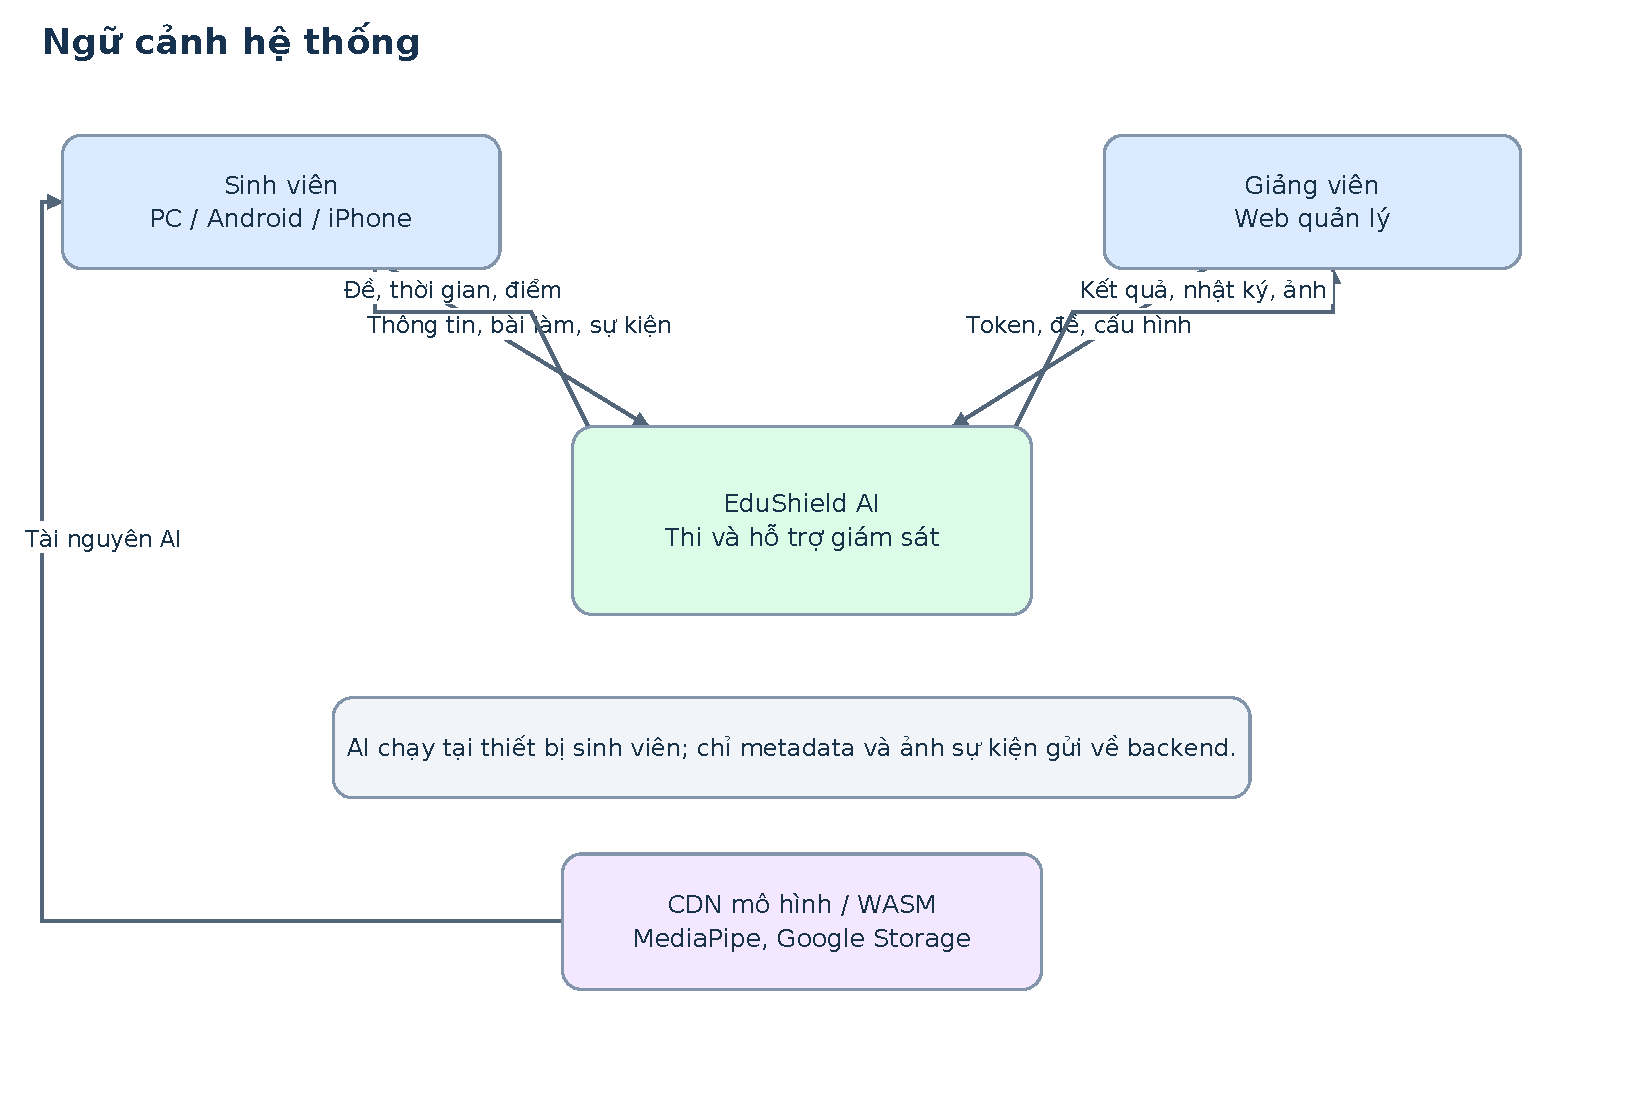
\includegraphics[width=\textwidth,height=0.70\textheight,keepaspectratio]{diagrams/01-context.pdf}
\caption{Ngữ cảnh hệ thống của EduShield AI.}\label{fig:01-context}
\end{figure}

\clearpage
\subsection{Ca sử dụng chính}
Ca sử dụng bao quát thao tác của sinh viên và giảng viên. Chọn vai trò ở giao diện không cấp quyền quản lý; backend vẫn xác minh token.
\begin{figure}[H]
\centering
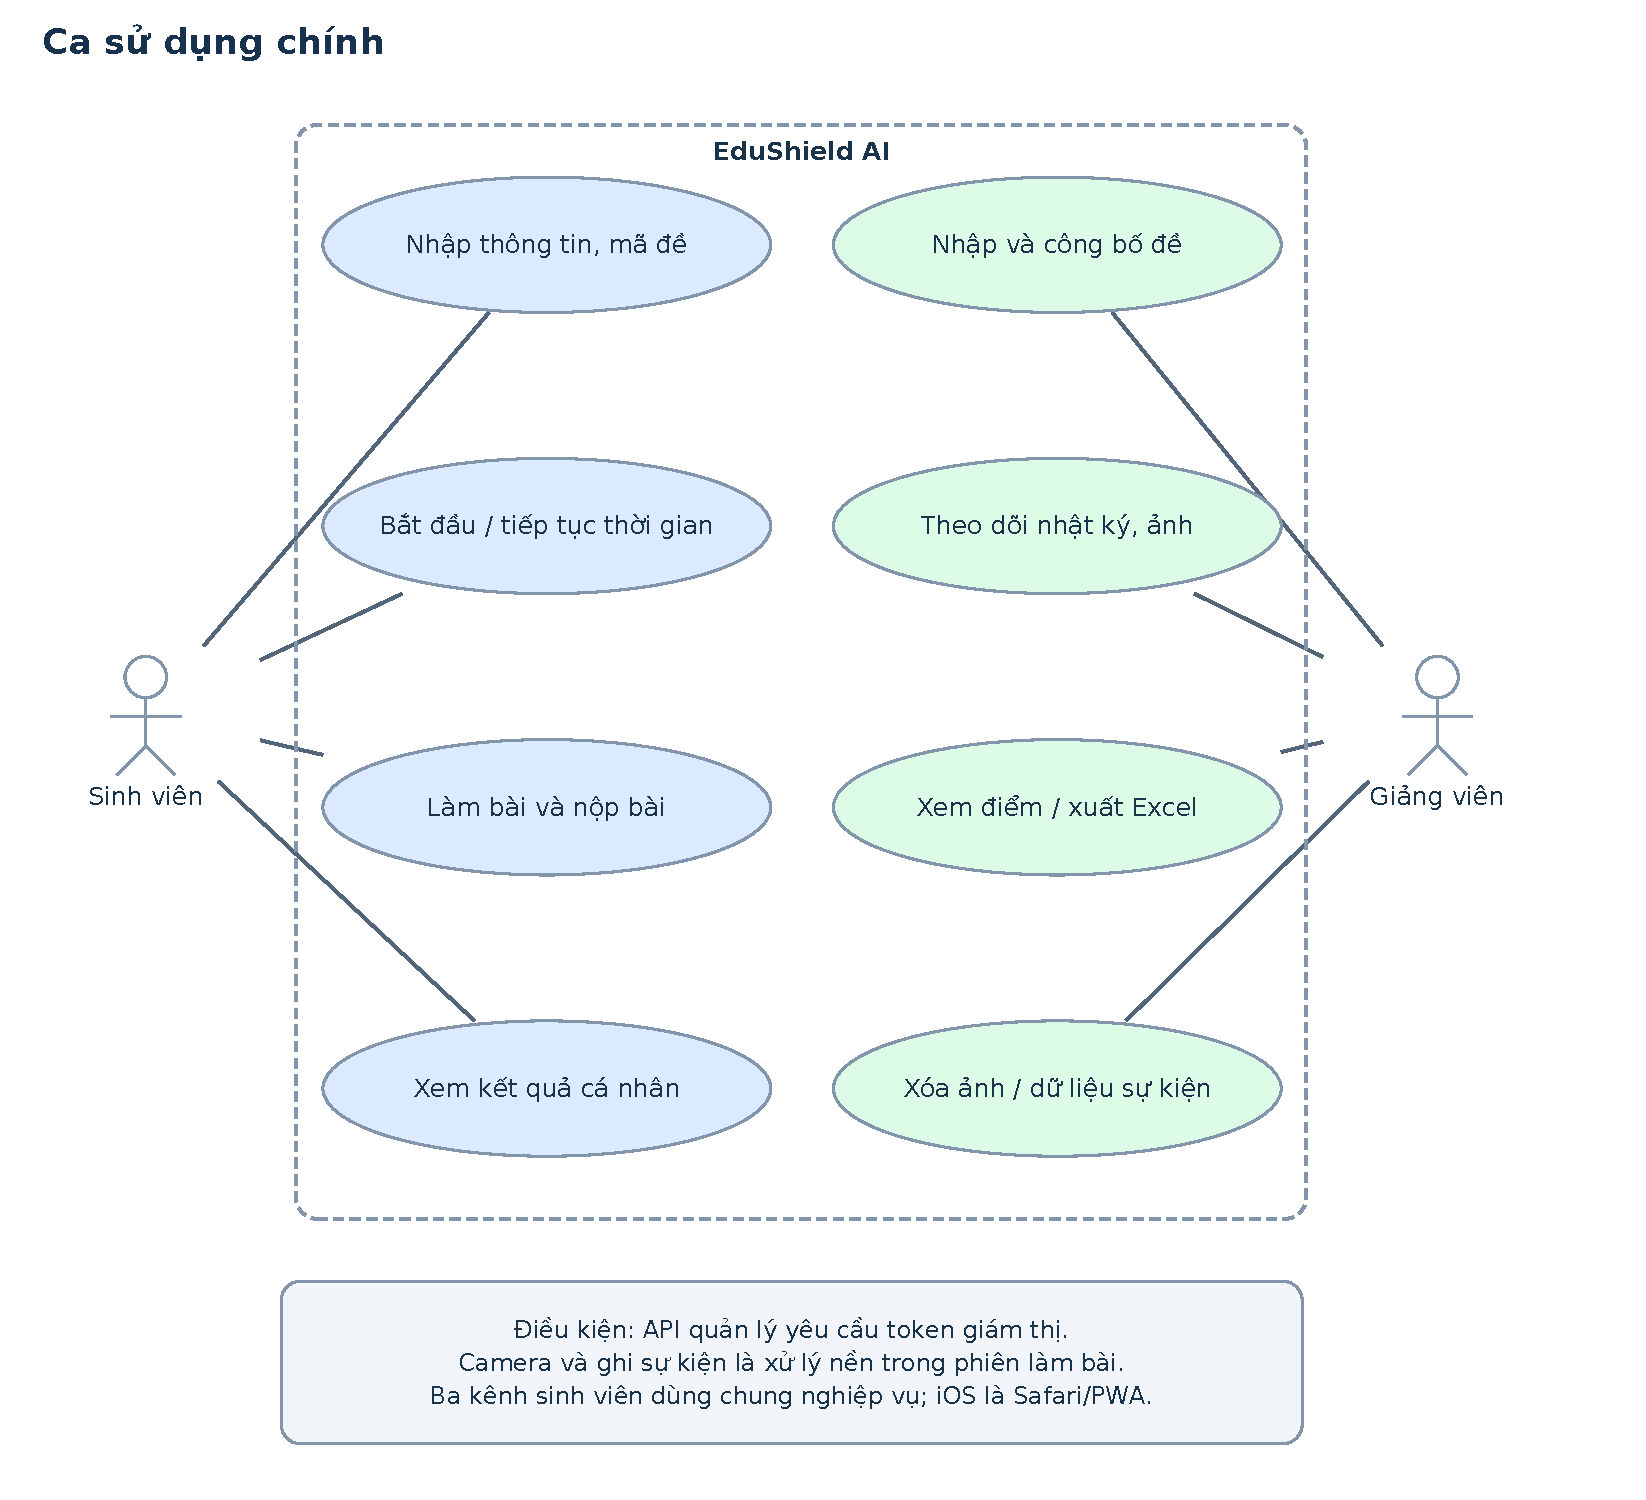
\includegraphics[width=\textwidth,height=0.70\textheight,keepaspectratio]{diagrams/02-usecase.pdf}
\caption{Ca sử dụng chính của EduShield AI.}\label{fig:02-usecase}
\end{figure}

\clearpage
\subsection{Cấu trúc thành phần}
Sơ đồ thành phần thể hiện trách nhiệm chính và phụ thuộc mức mô-đun, không phải sơ đồ mọi lời gọi hàm. Các máy khách chia sẻ API nghiệp vụ.
\begin{figure}[H]
\centering
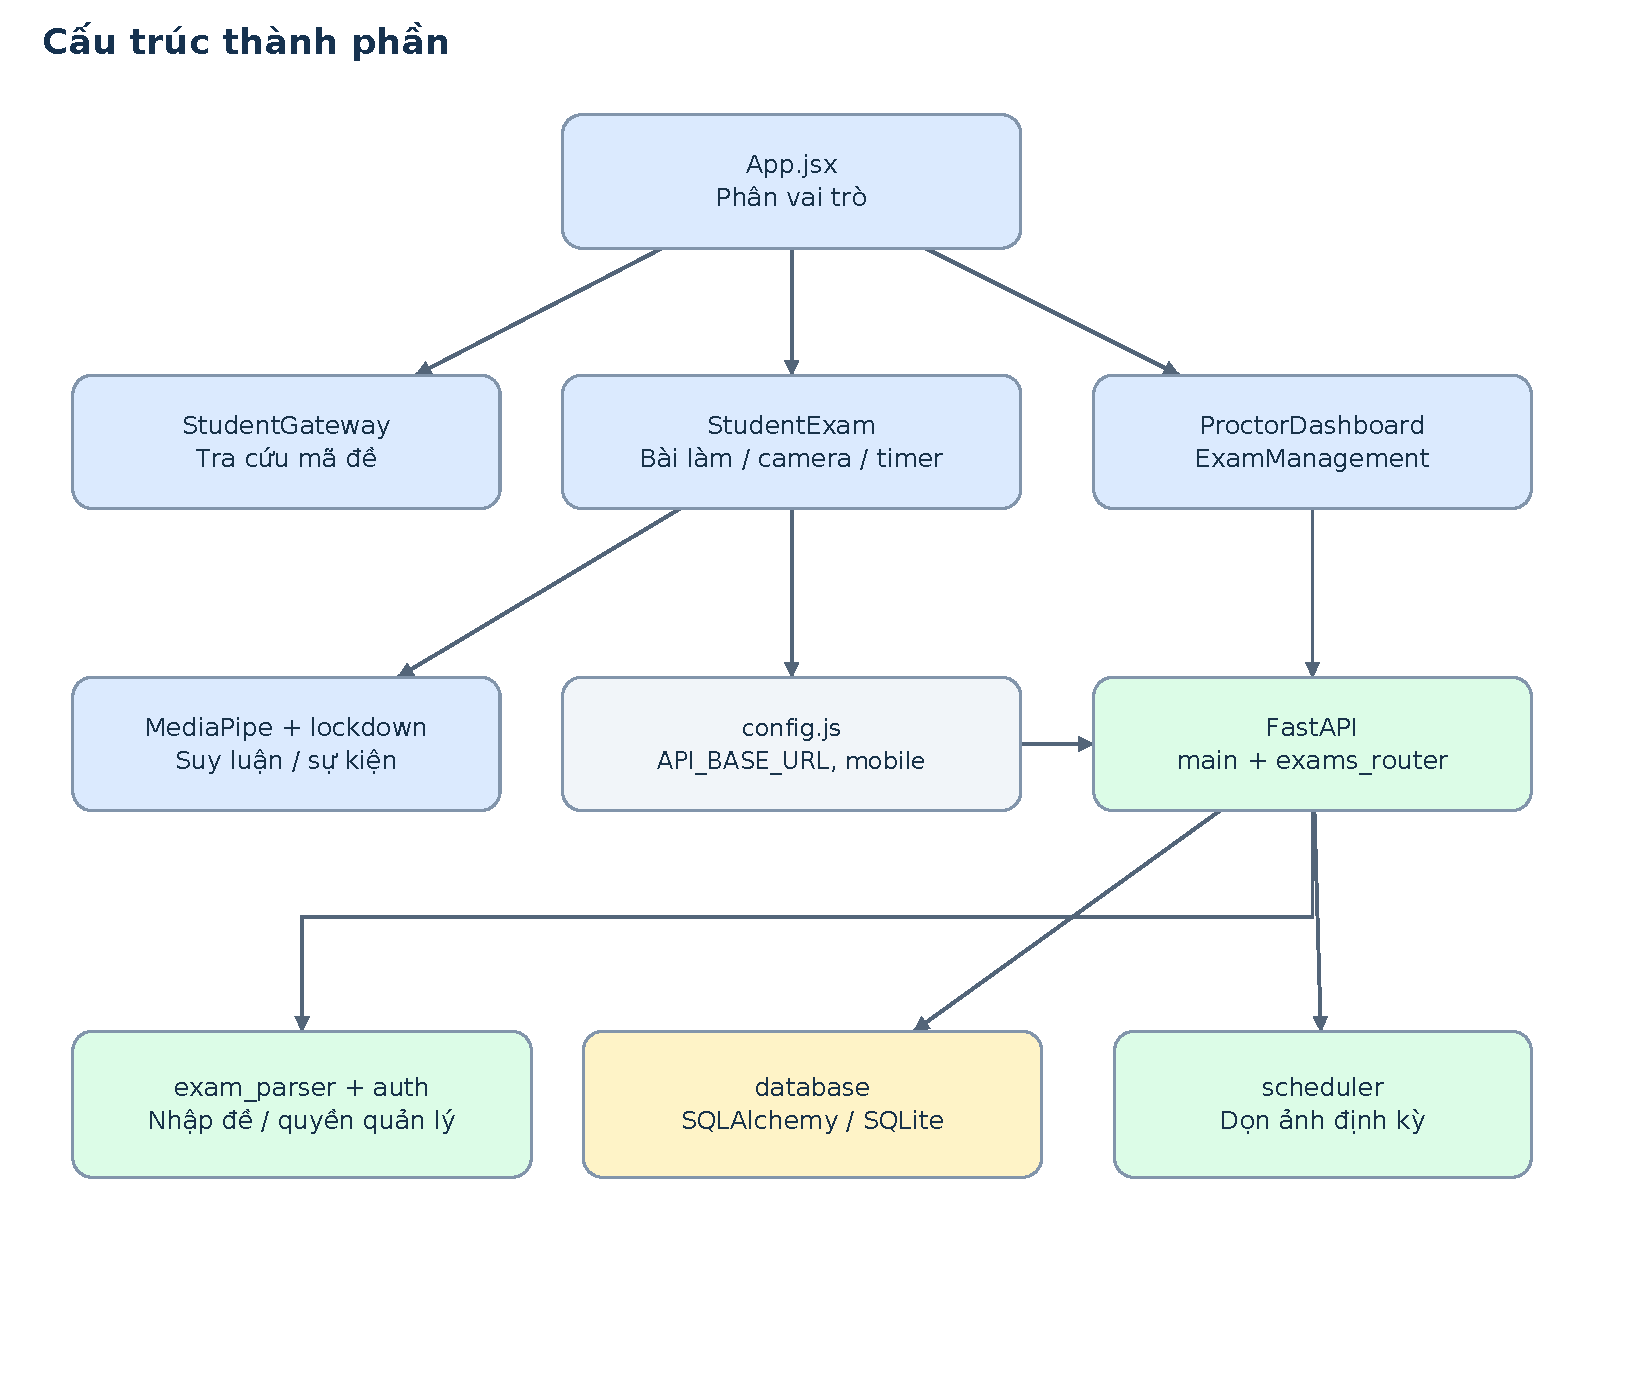
\includegraphics[width=\textwidth,height=0.70\textheight,keepaspectratio]{diagrams/03-components.pdf}
\caption{Cấu trúc thành phần của EduShield AI.}\label{fig:03-components}
\end{figure}

\clearpage
\subsection{Triển khai HTTPS đa thiết bị}
Web và API được phục vụ cùng origin trên FastAPI. APK là kênh đã chạy theo xác nhận tác giả nhưng chưa có nguồn native để tái lập trong repo main. iOS là Safari/PWA.
\begin{figure}[H]
\centering
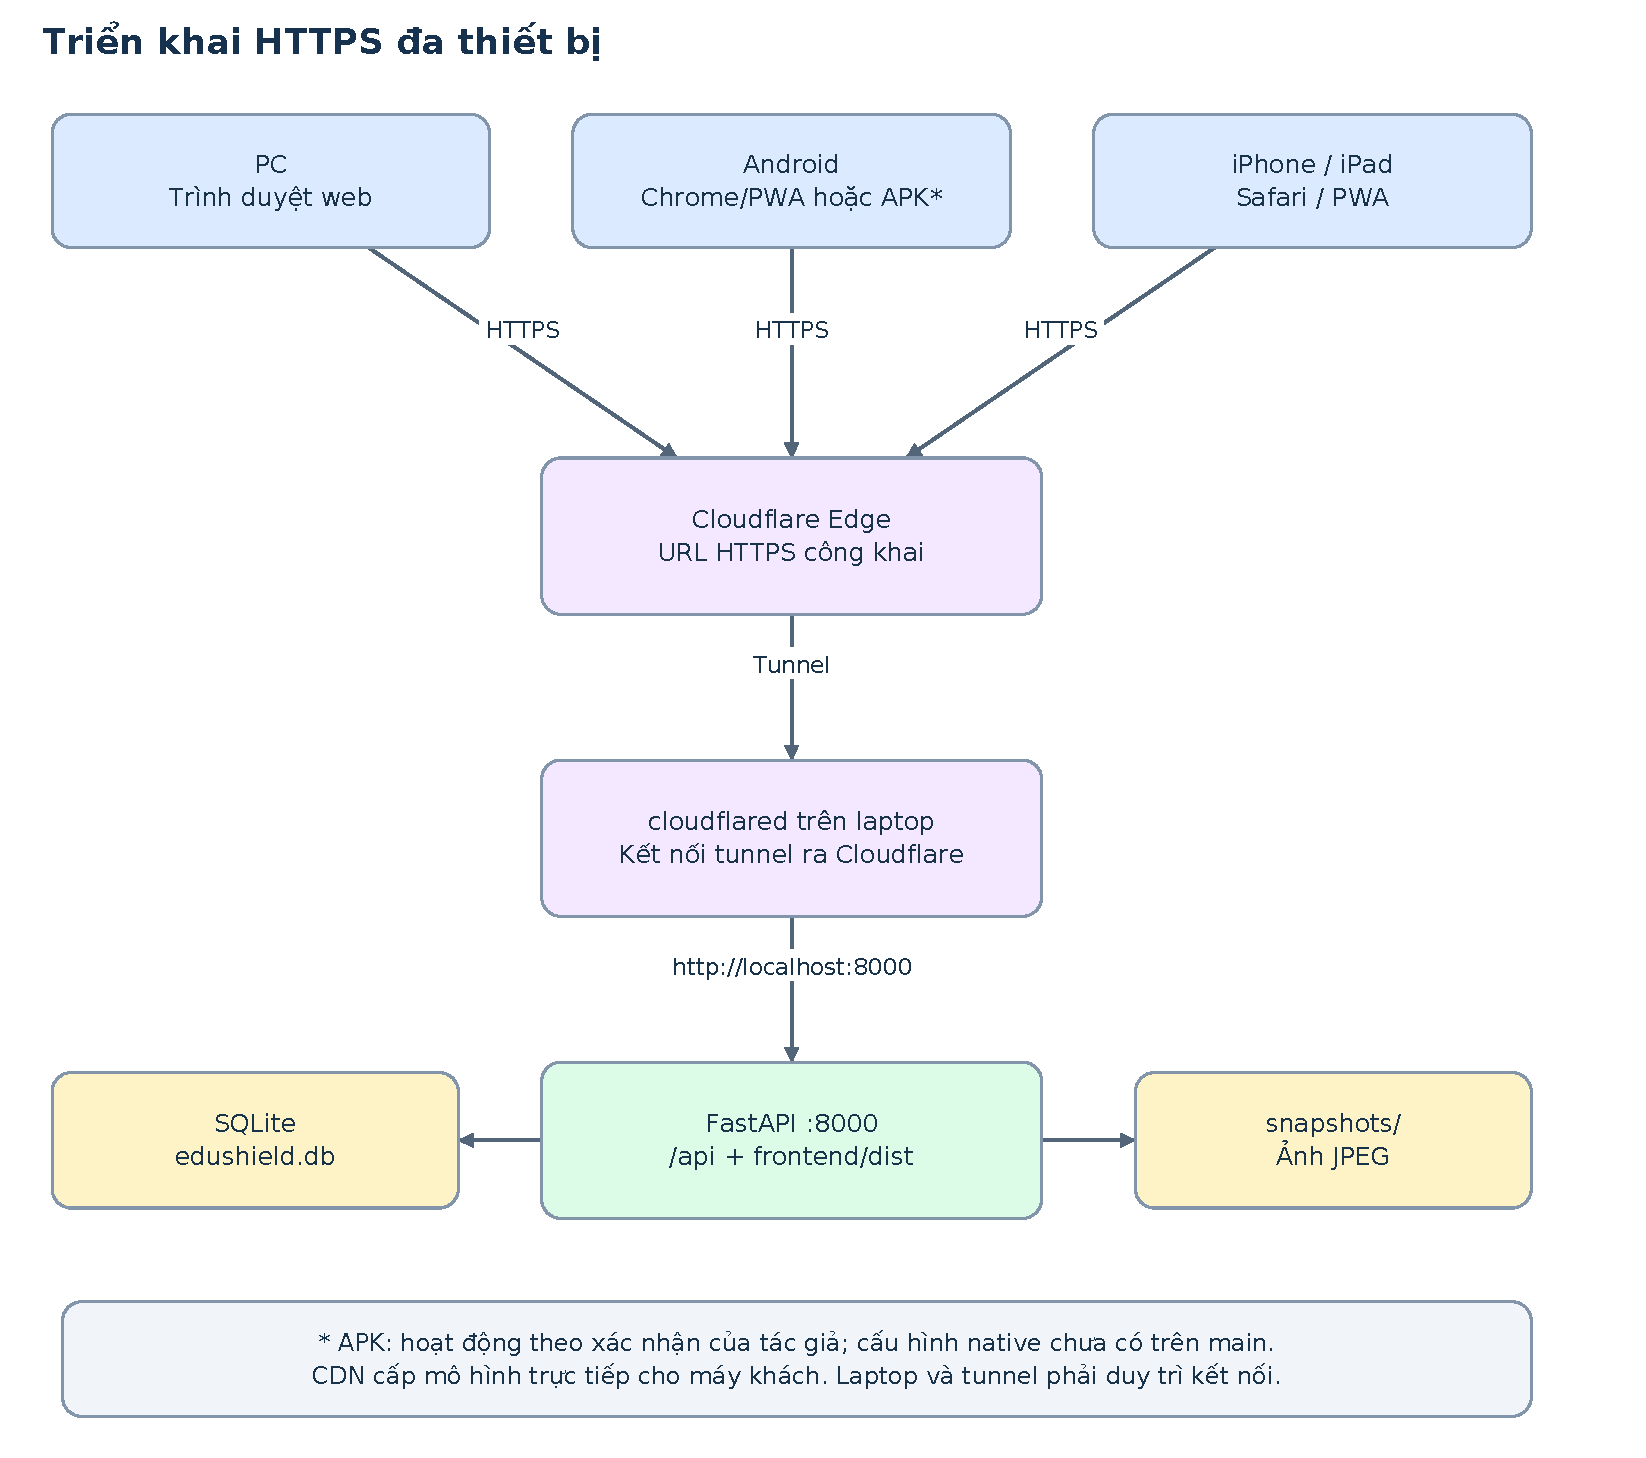
\includegraphics[width=\textwidth,height=0.70\textheight,keepaspectratio]{diagrams/04-deployment.pdf}
\caption{Triển khai HTTPS đa thiết bị của EduShield AI.}\label{fig:04-deployment}
\end{figure}

\clearpage
\subsection{Luồng dữ liệu mức 1}
DFD mức 1 phân rã các xử lý nghiệp vụ và kho dữ liệu. Suy luận hình ảnh nằm ở máy khách; backend nhận sự kiện đã xử lý thay vì nhận luồng video liên tục.
\begin{figure}[H]
\centering
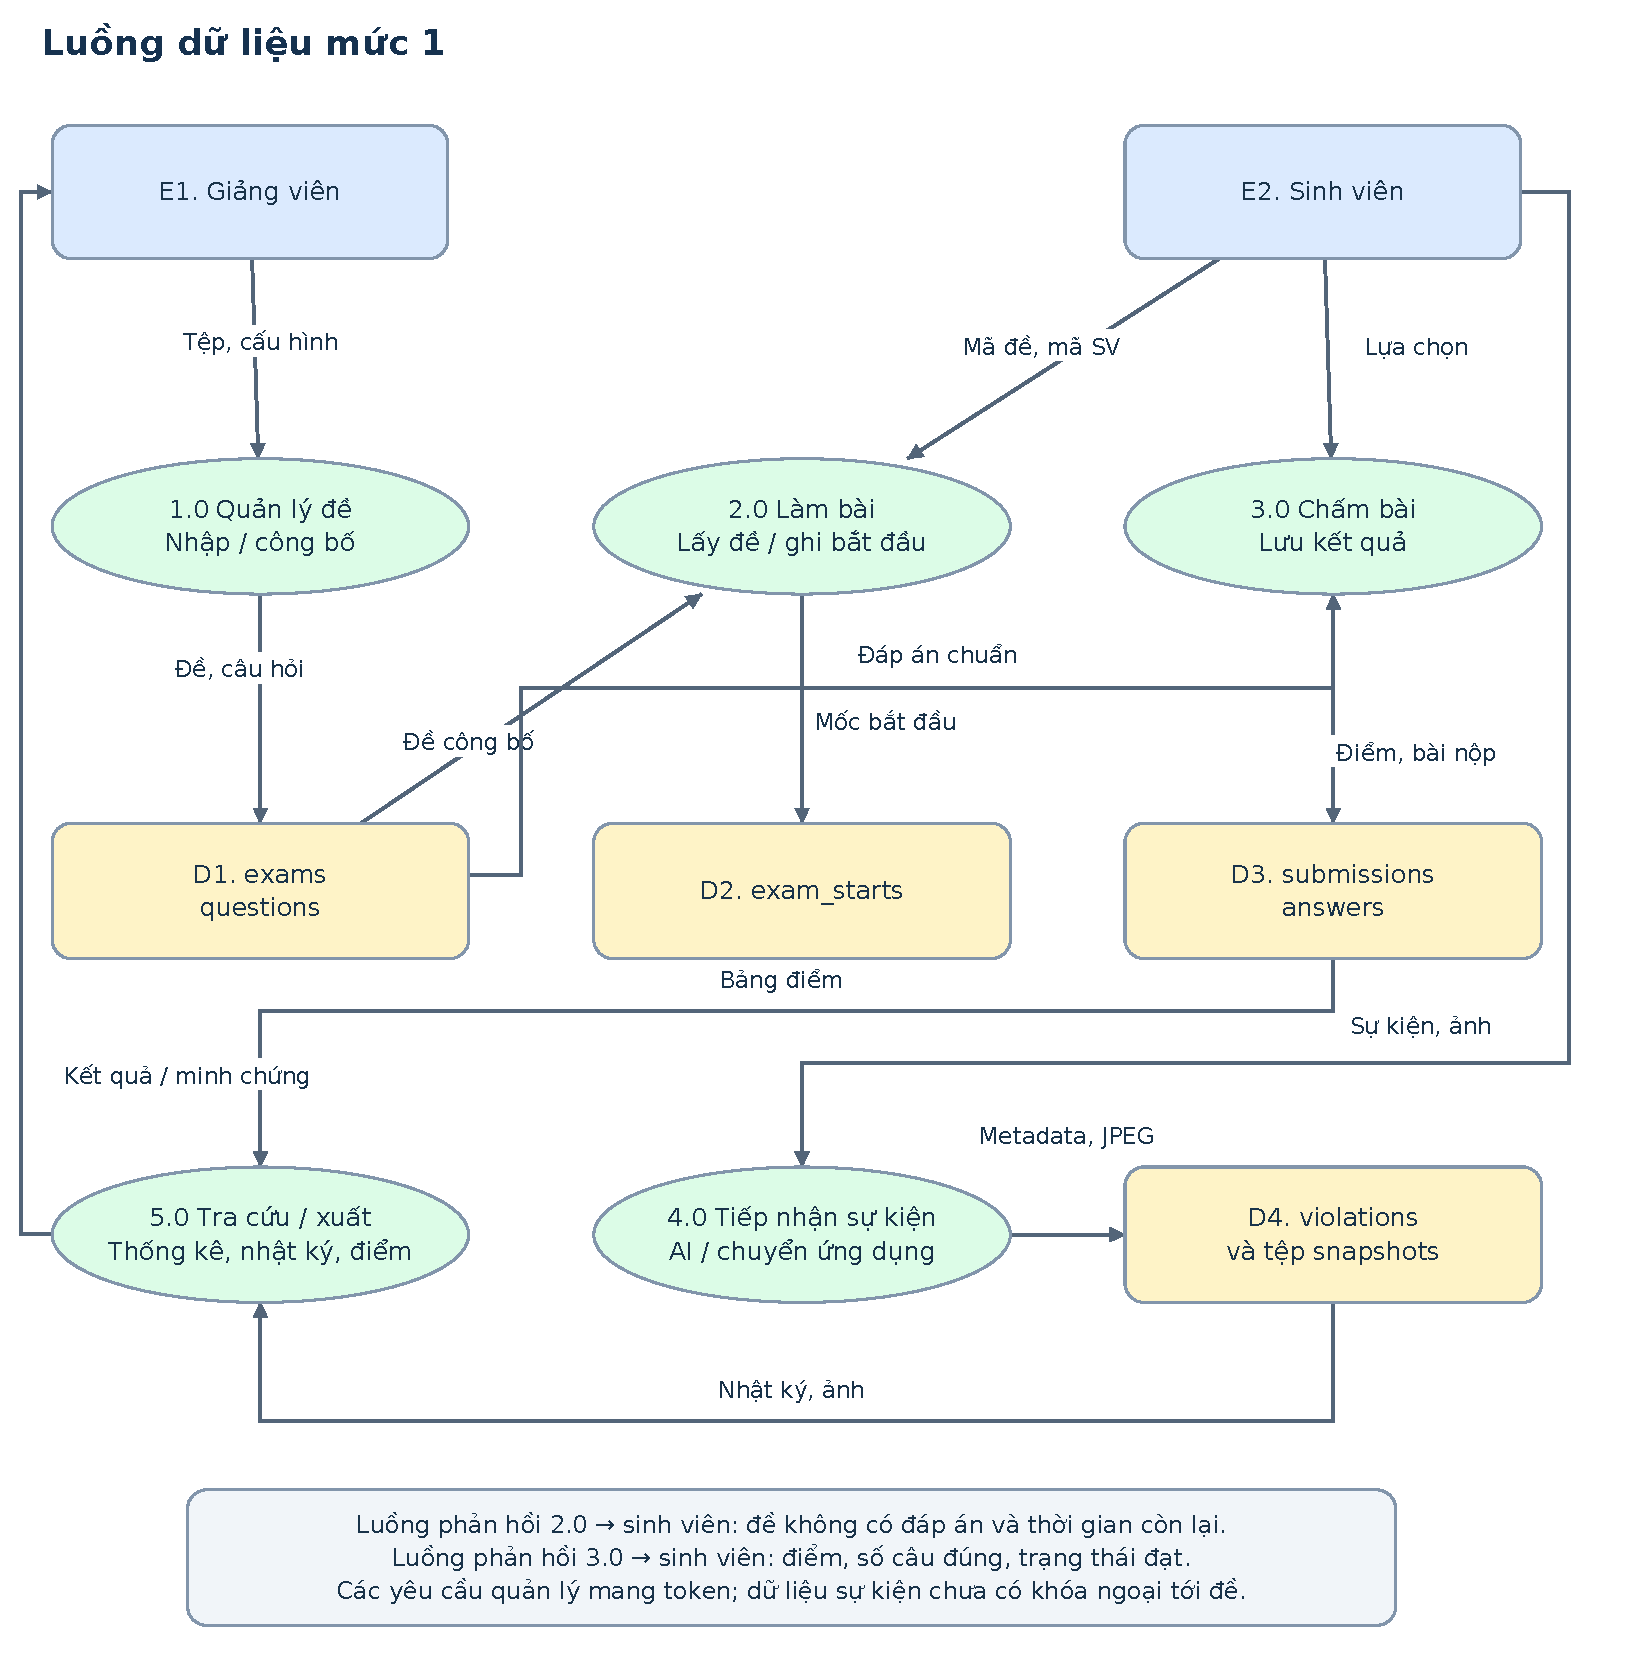
\includegraphics[width=\textwidth,height=0.70\textheight,keepaspectratio]{diagrams/05-dfd.pdf}
\caption{Luồng dữ liệu mức 1 của EduShield AI.}\label{fig:05-dfd}
\end{figure}

\clearpage
\subsection{Mô hình dữ liệu quan hệ}
ERD bổ sung exam\_starts và các quan hệ khóa ngoại thực tế. Đường đứt tới violations là phép ghép logic theo mã sinh viên và thời gian, không phải quan hệ được CSDL cưỡng chế.
\begin{figure}[H]
\centering
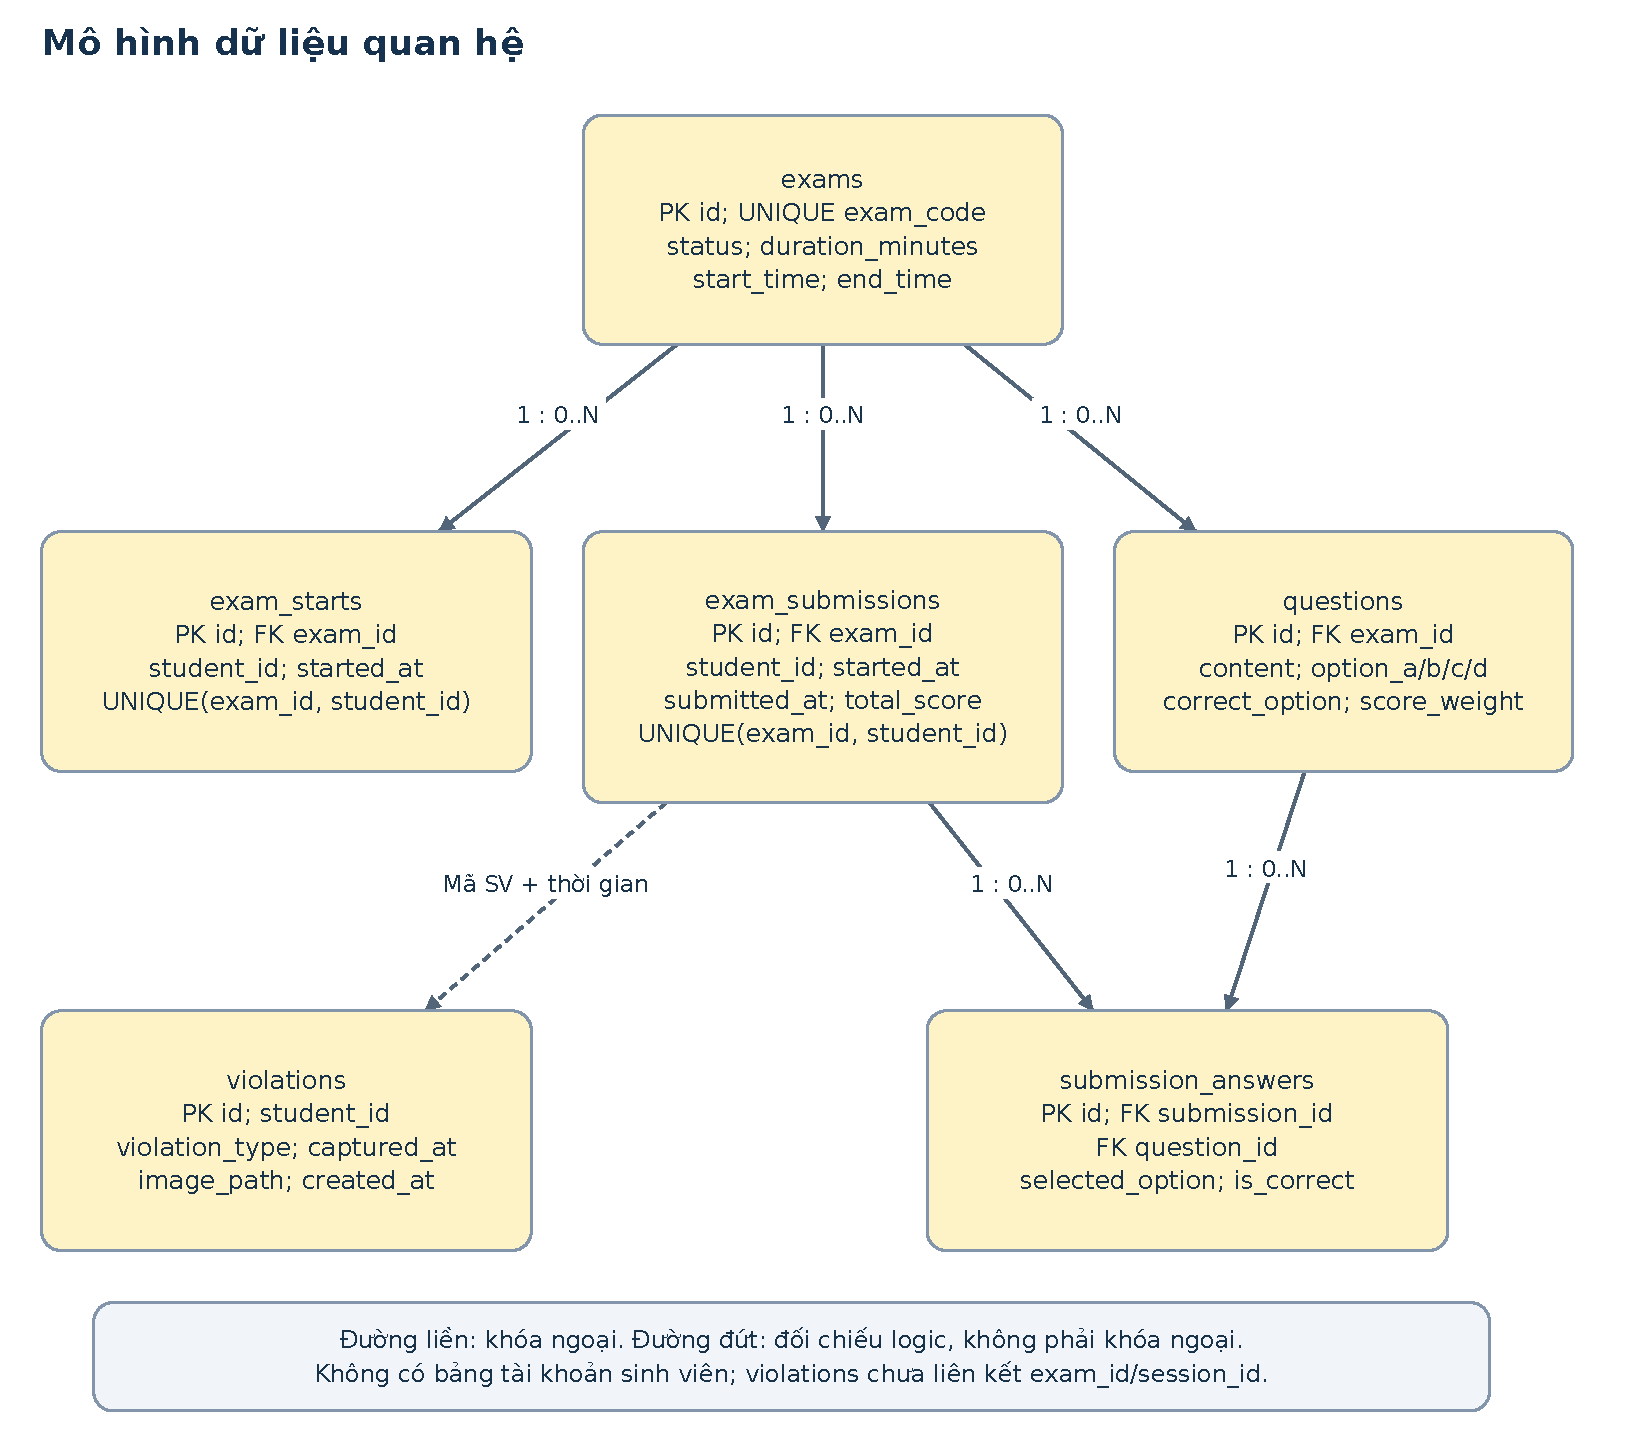
\includegraphics[width=\textwidth,height=0.70\textheight,keepaspectratio]{diagrams/06-erd.pdf}
\caption{Mô hình dữ liệu quan hệ của EduShield AI.}\label{fig:06-erd}
\end{figure}

\clearpage
\subsection{Luồng hoạt động toàn hệ thống}
Luồng tổng thể nối việc chuẩn bị đề và tunnel với quá trình làm bài, giám sát song song, nộp và tra cứu kết quả. Các nhánh lỗi mạng/camera được giải thích ở phần triển khai và kiểm thử.
\begin{figure}[H]
\centering
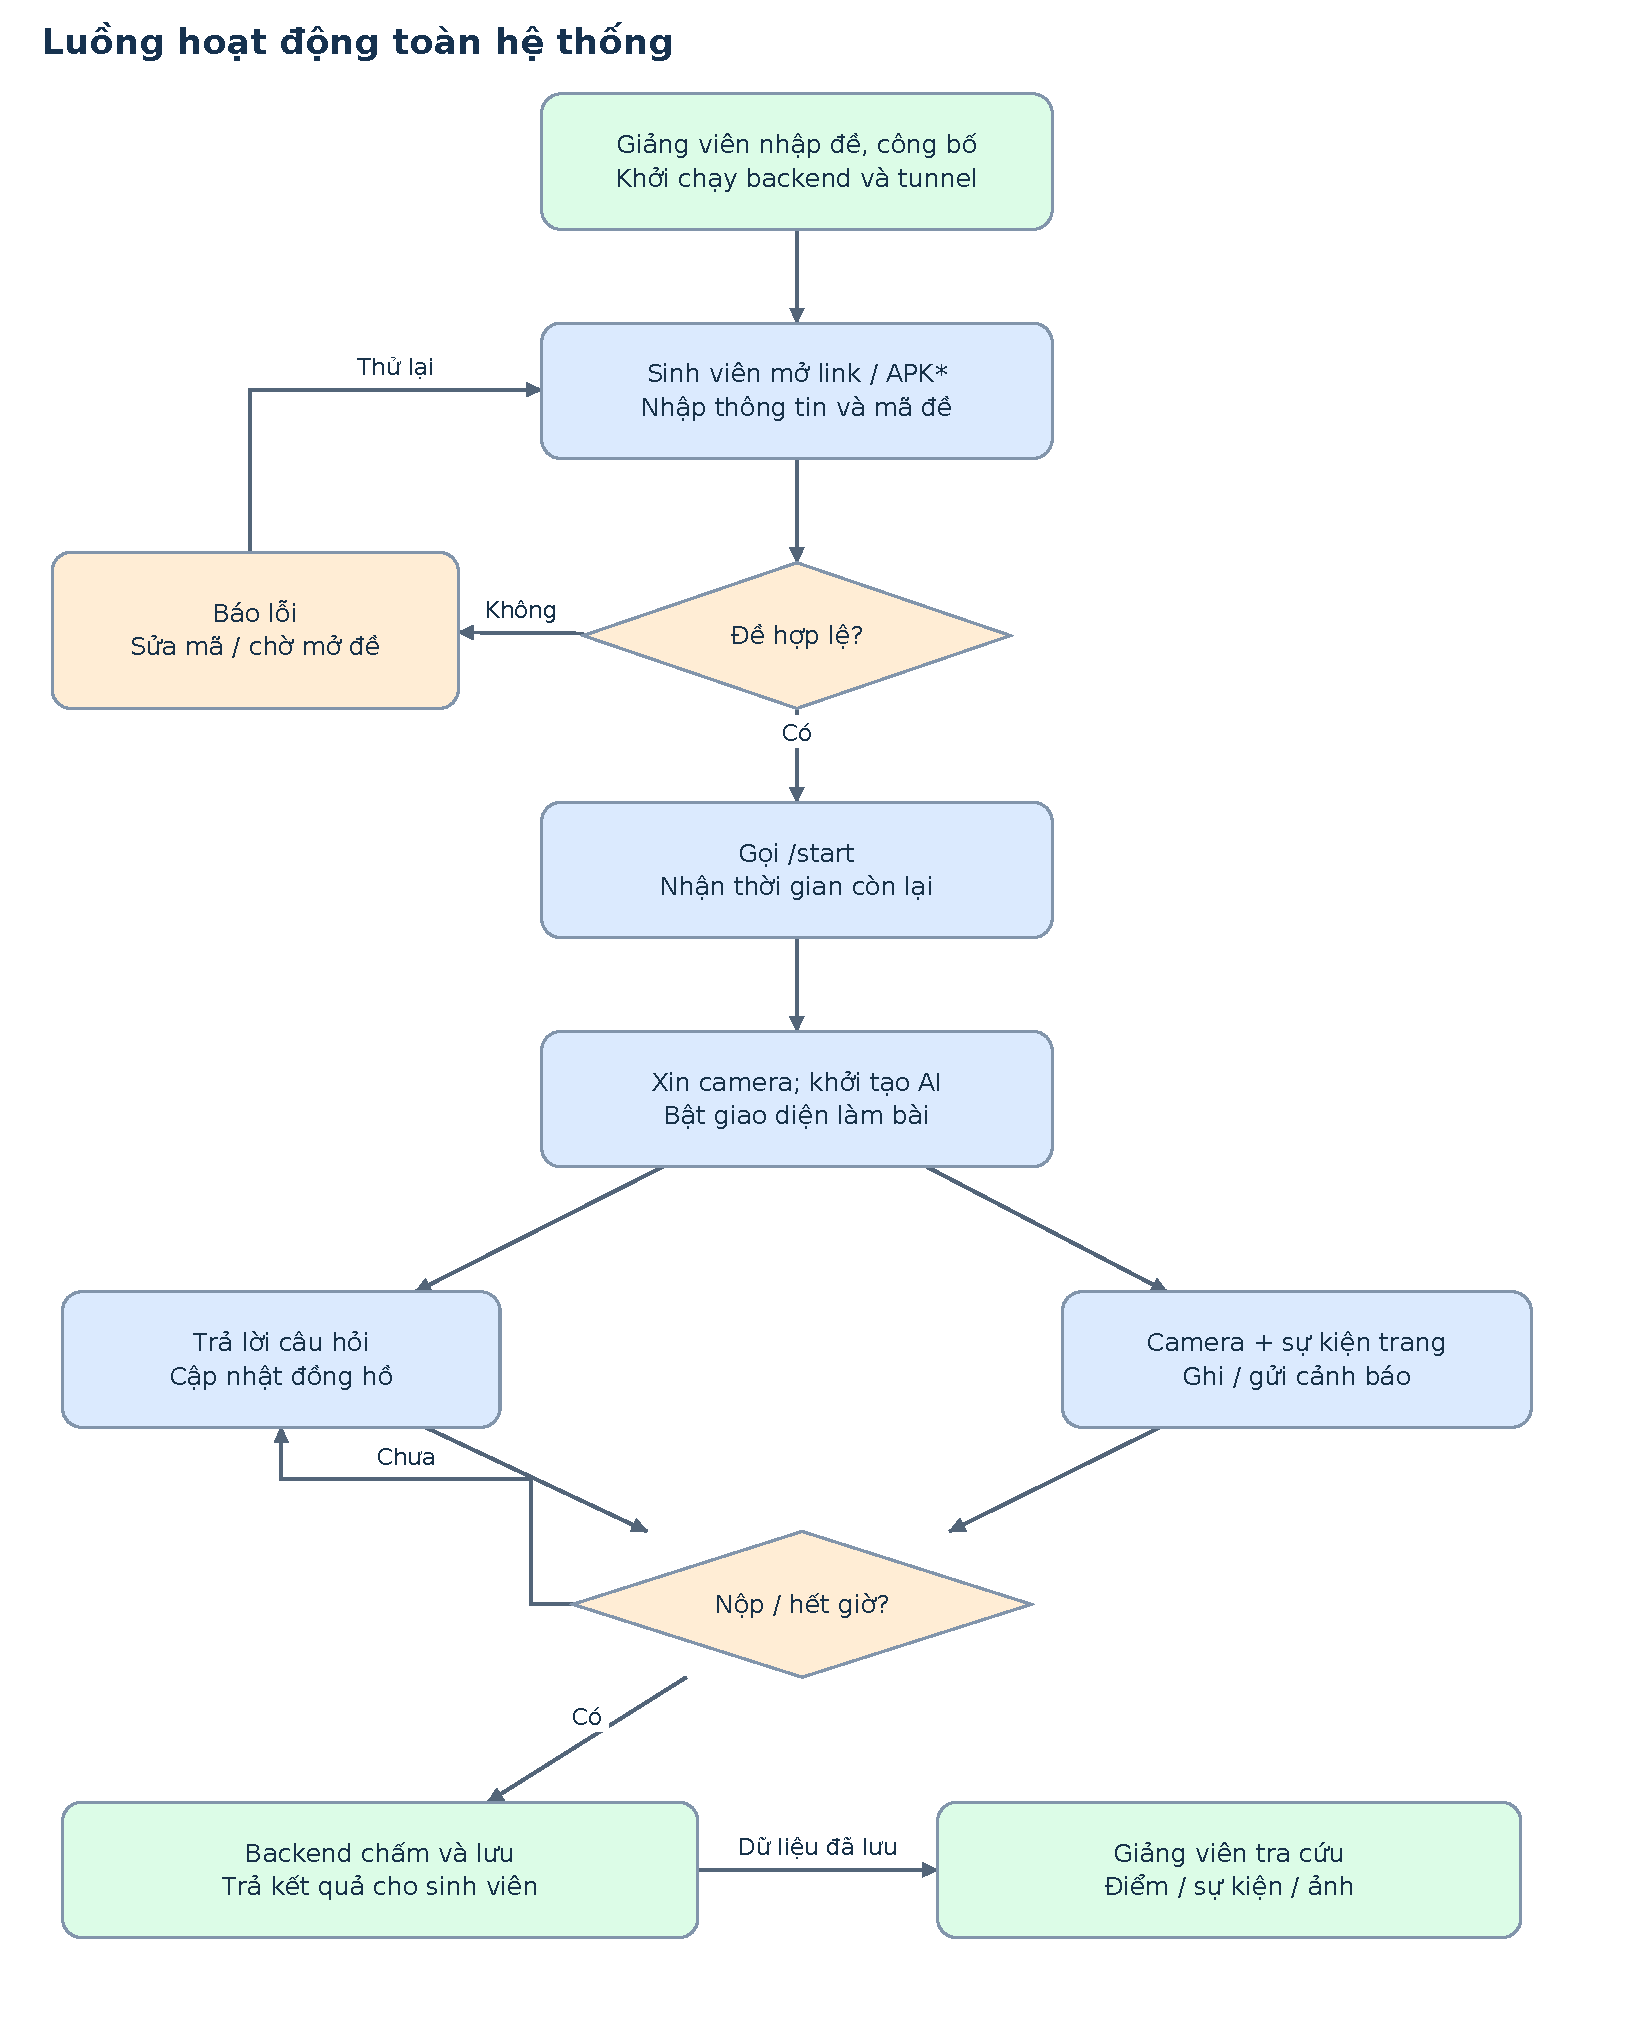
\includegraphics[width=\textwidth,height=0.70\textheight,keepaspectratio]{diagrams/07-activity.pdf}
\caption{Luồng hoạt động toàn hệ thống của EduShield AI.}\label{fig:07-activity}
\end{figure}

\clearpage
\subsection{Tuần tự bắt đầu và tiếp tục thời gian}
Thời gian còn lại do API start tính từ lần bắt đầu đầu tiên. Việc vào lại không phục hồi lựa chọn cũ; nhánh fallback vẫn cấp đủ thời lượng nếu API lỗi ngoài các trạng thái chặn đã nêu.
\begin{figure}[H]
\centering
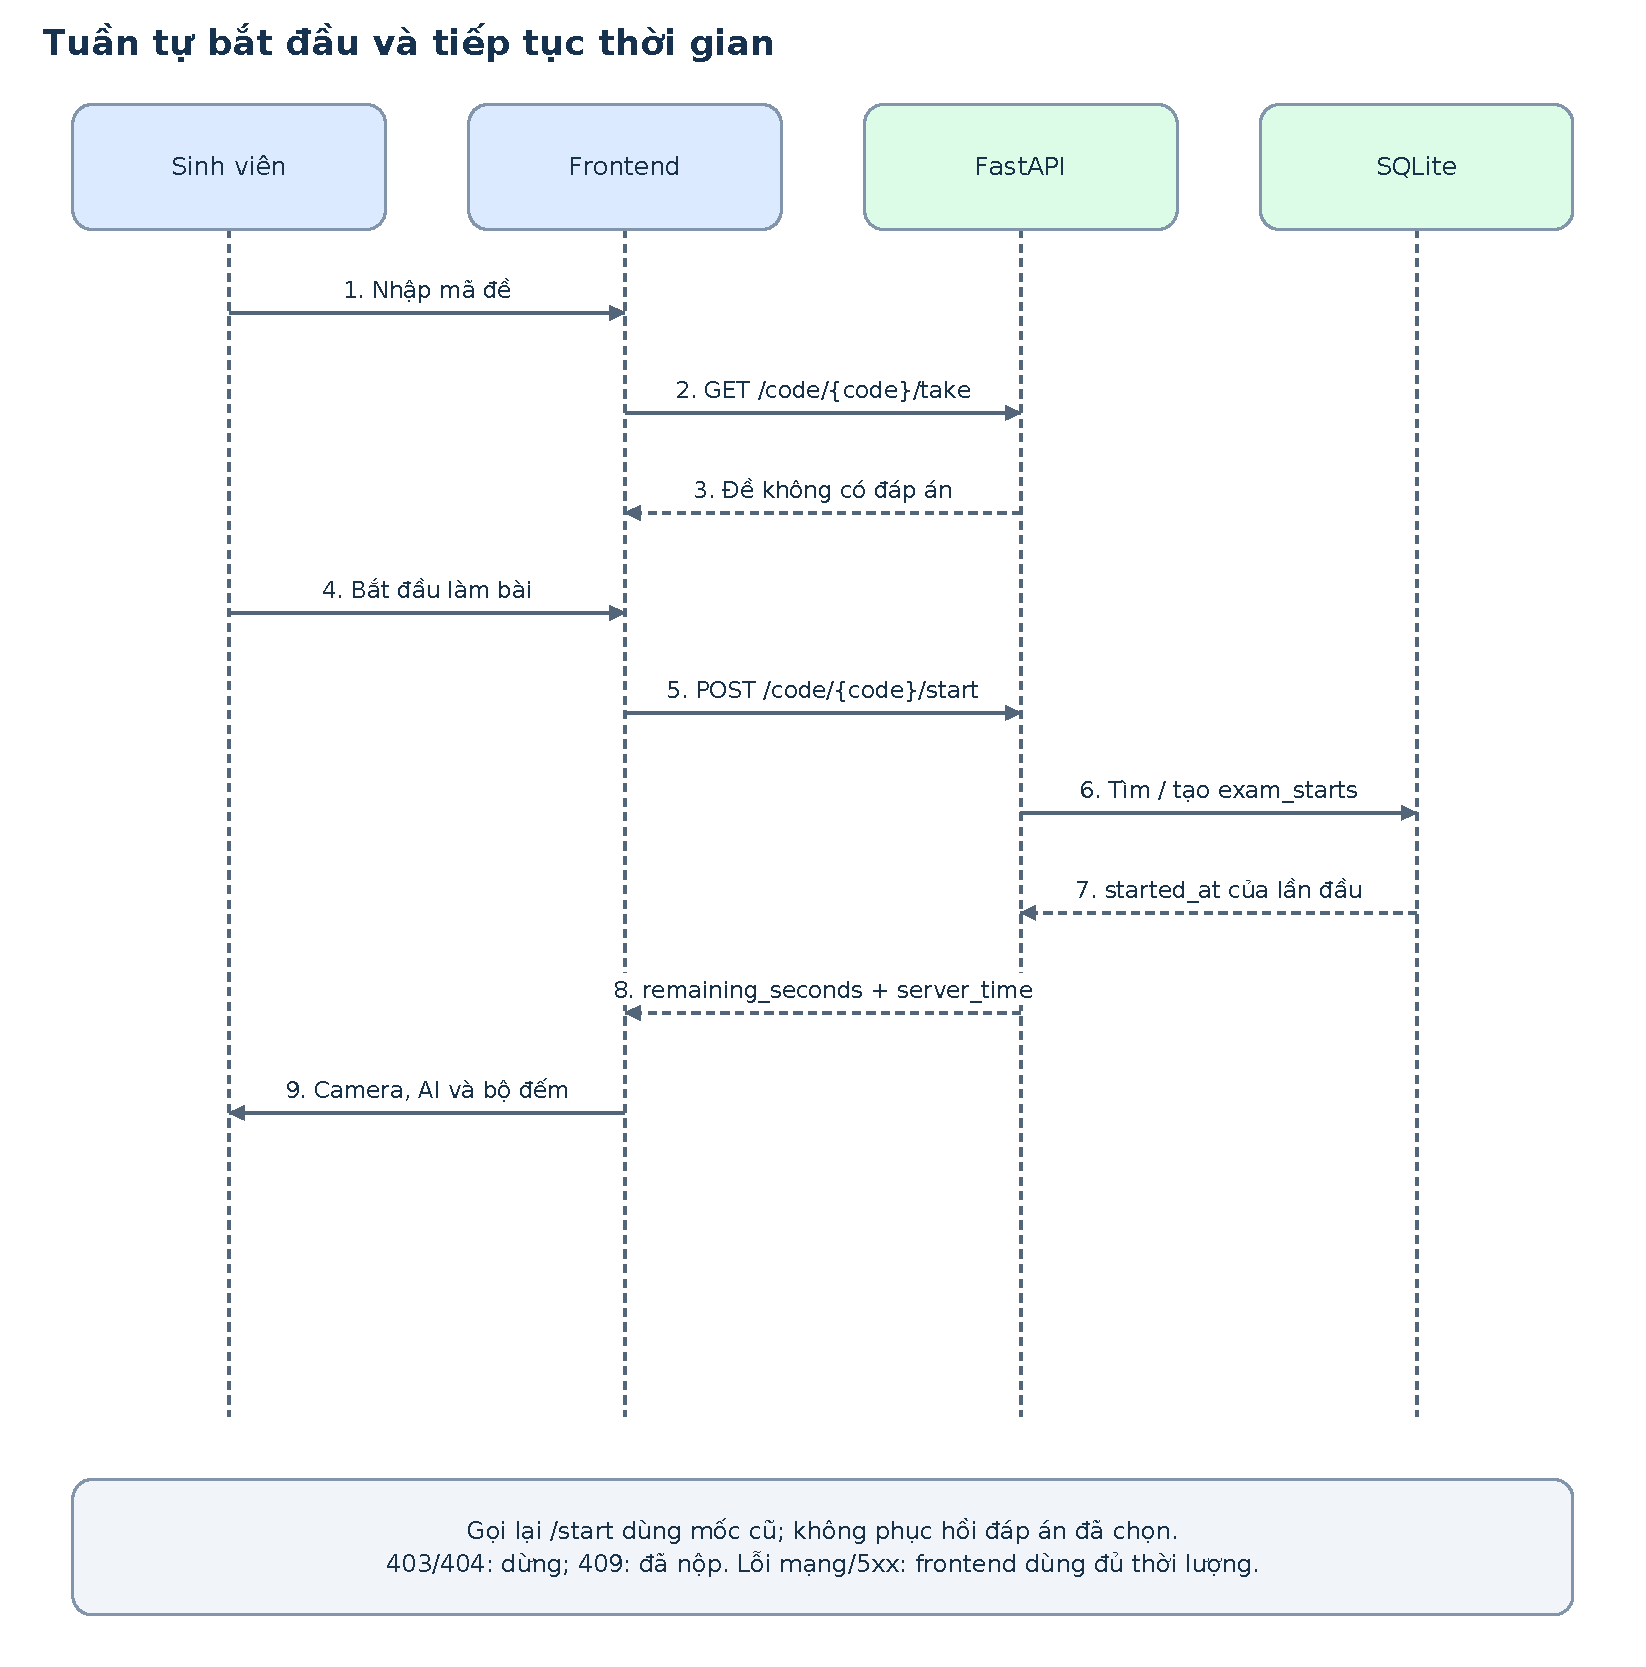
\includegraphics[width=\textwidth,height=0.70\textheight,keepaspectratio]{diagrams/08-seq-start.pdf}
\caption{Tuần tự bắt đầu và tiếp tục thời gian của EduShield AI.}\label{fig:08-seq-start}
\end{figure}

\clearpage
\subsection{Tuần tự ghi sự kiện và xem minh chứng}
Giảng viên đọc sự kiện bằng polling, không dùng WebSocket. Khi chuyển ứng dụng, camera có thể không cung cấp được ảnh; payload vẫn cho phép metadata không kèm ảnh.
\begin{figure}[H]
\centering
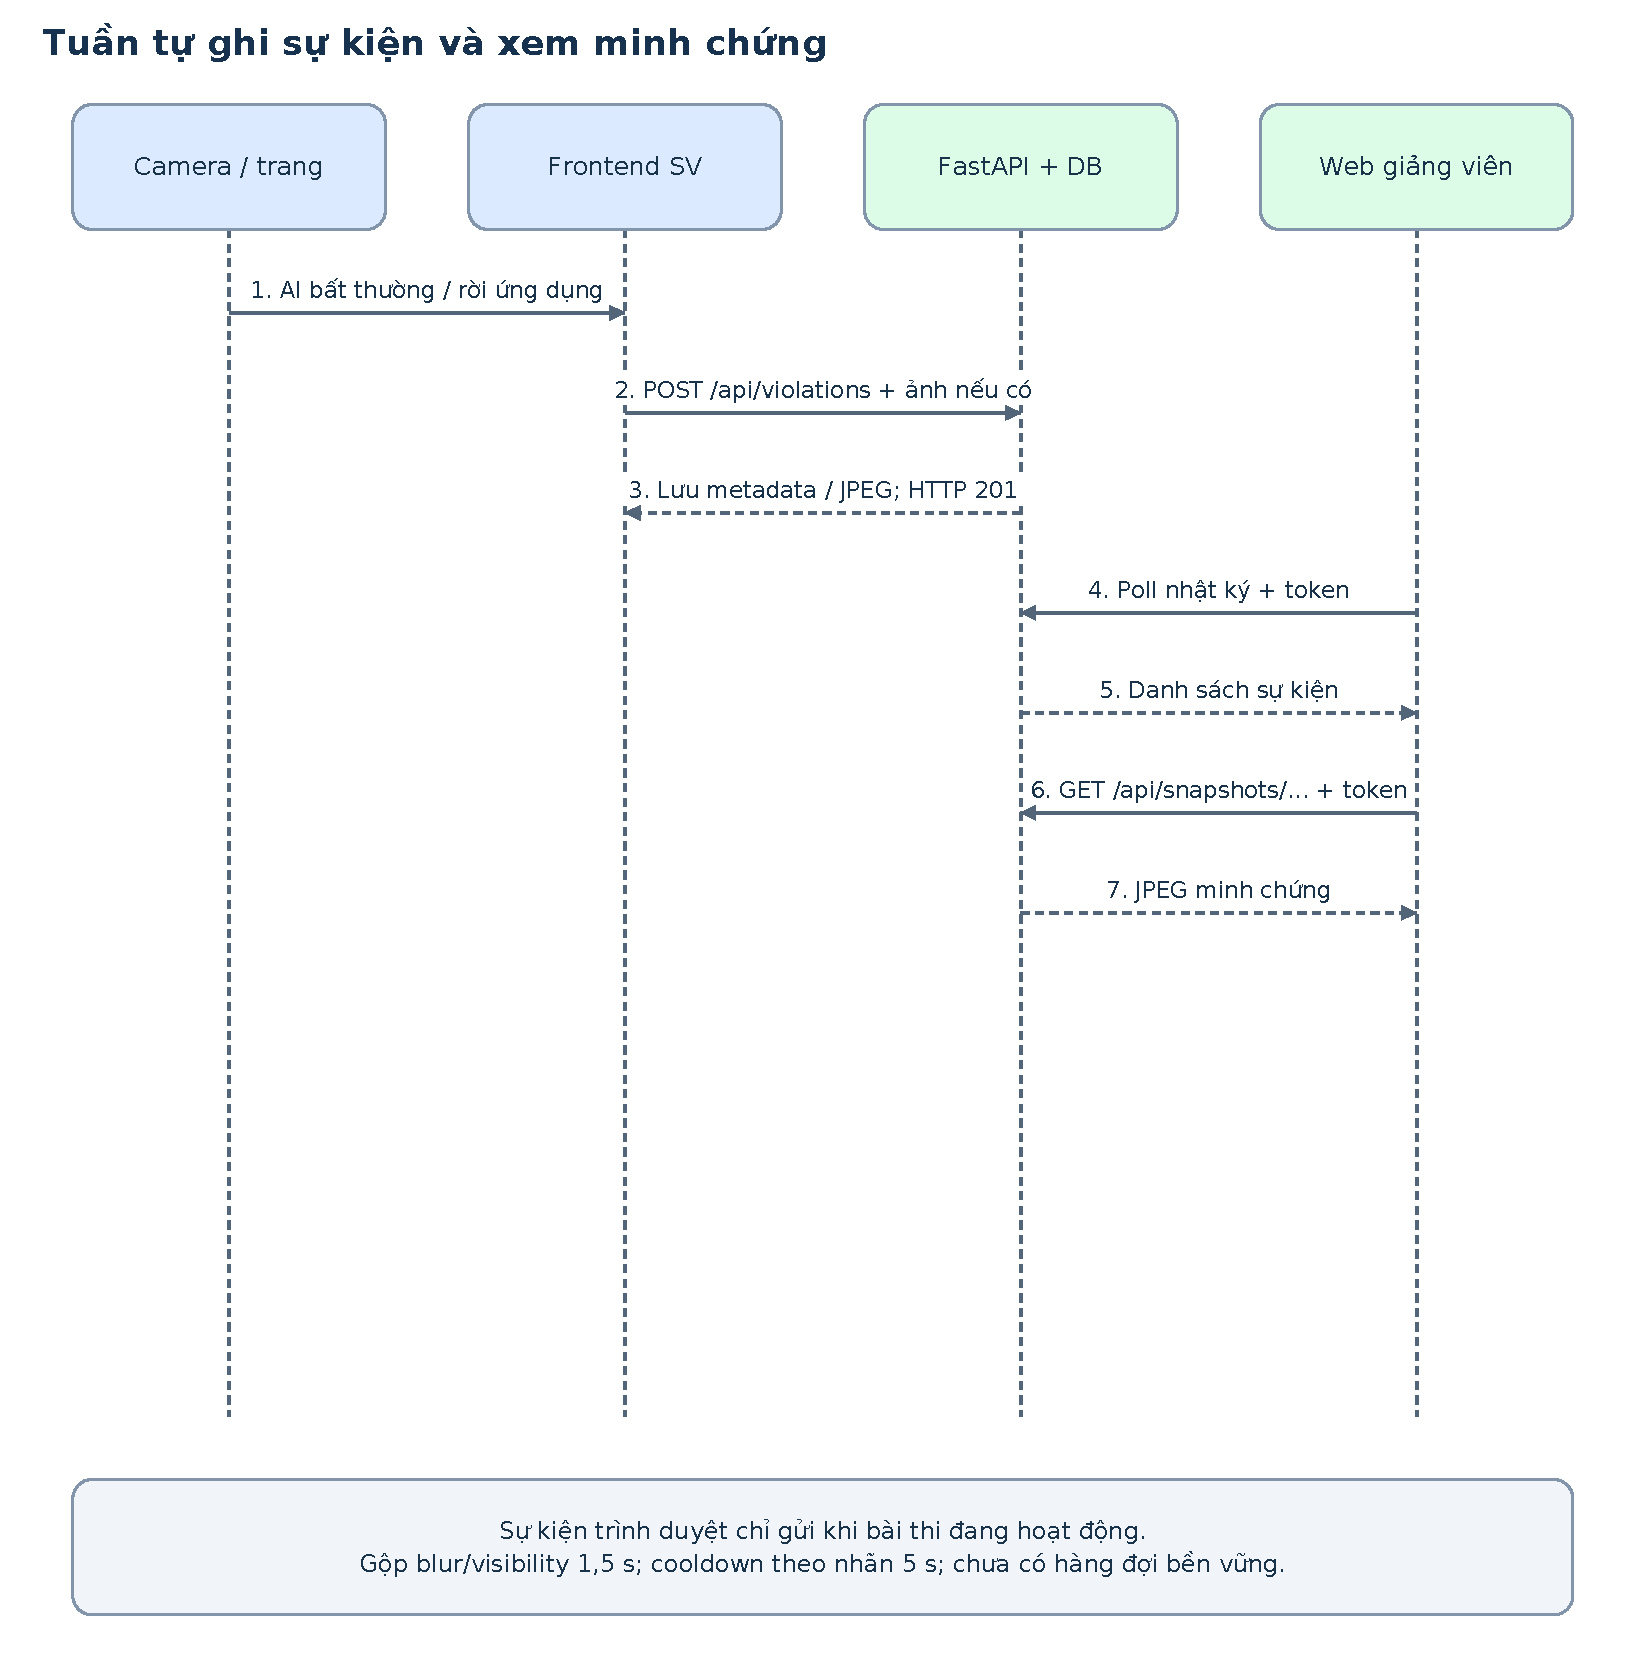
\includegraphics[width=\textwidth,height=0.70\textheight,keepaspectratio]{diagrams/09-seq-event.pdf}
\caption{Tuần tự ghi sự kiện và xem minh chứng của EduShield AI.}\label{fig:09-seq-event}
\end{figure}

\clearpage
\subsection{Tuần tự nộp và chấm bài}
Điểm được tính từ đáp án trong CSDL và ghi cùng chi tiết bài nộp. UNIQUE chống trùng là lớp bảo vệ cuối cùng; deadline chưa được cưỡng chế tại submit.
\begin{figure}[H]
\centering
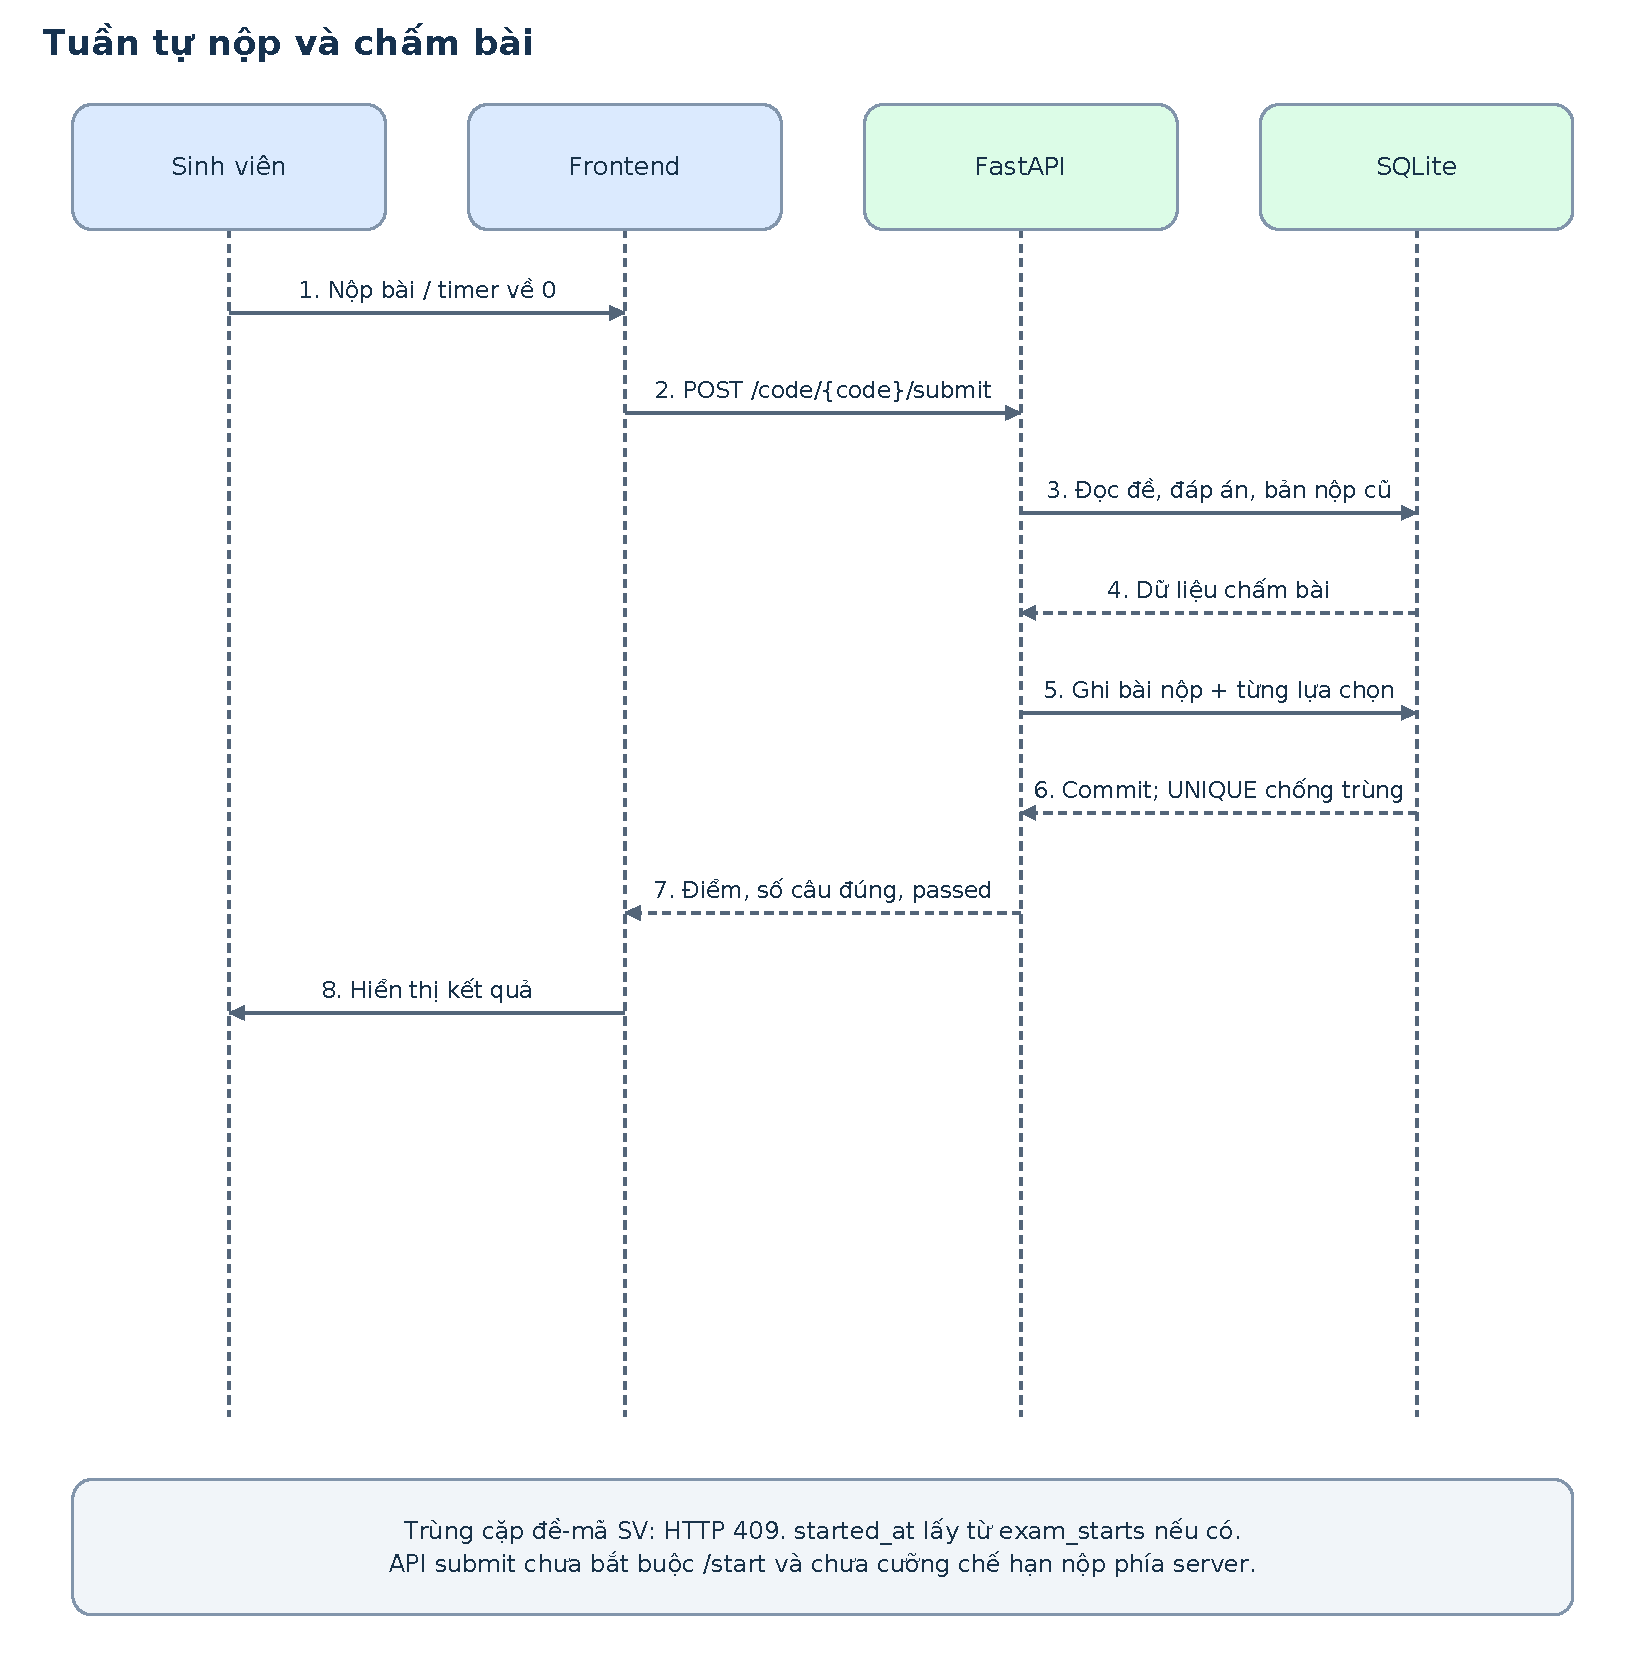
\includegraphics[width=\textwidth,height=0.70\textheight,keepaspectratio]{diagrams/10-seq-submit.pdf}
\caption{Tuần tự nộp và chấm bài của EduShield AI.}\label{fig:10-seq-submit}
\end{figure}

\clearpage
\subsection{Trạng thái tương tác của bài thi}
Đây là trạng thái tương tác của giao diện, không phải tập trạng thái lưu nguyên dạng trong CSDL. Xuống nền không có nghĩa là backend tạm dừng thời gian thi.
\begin{figure}[H]
\centering
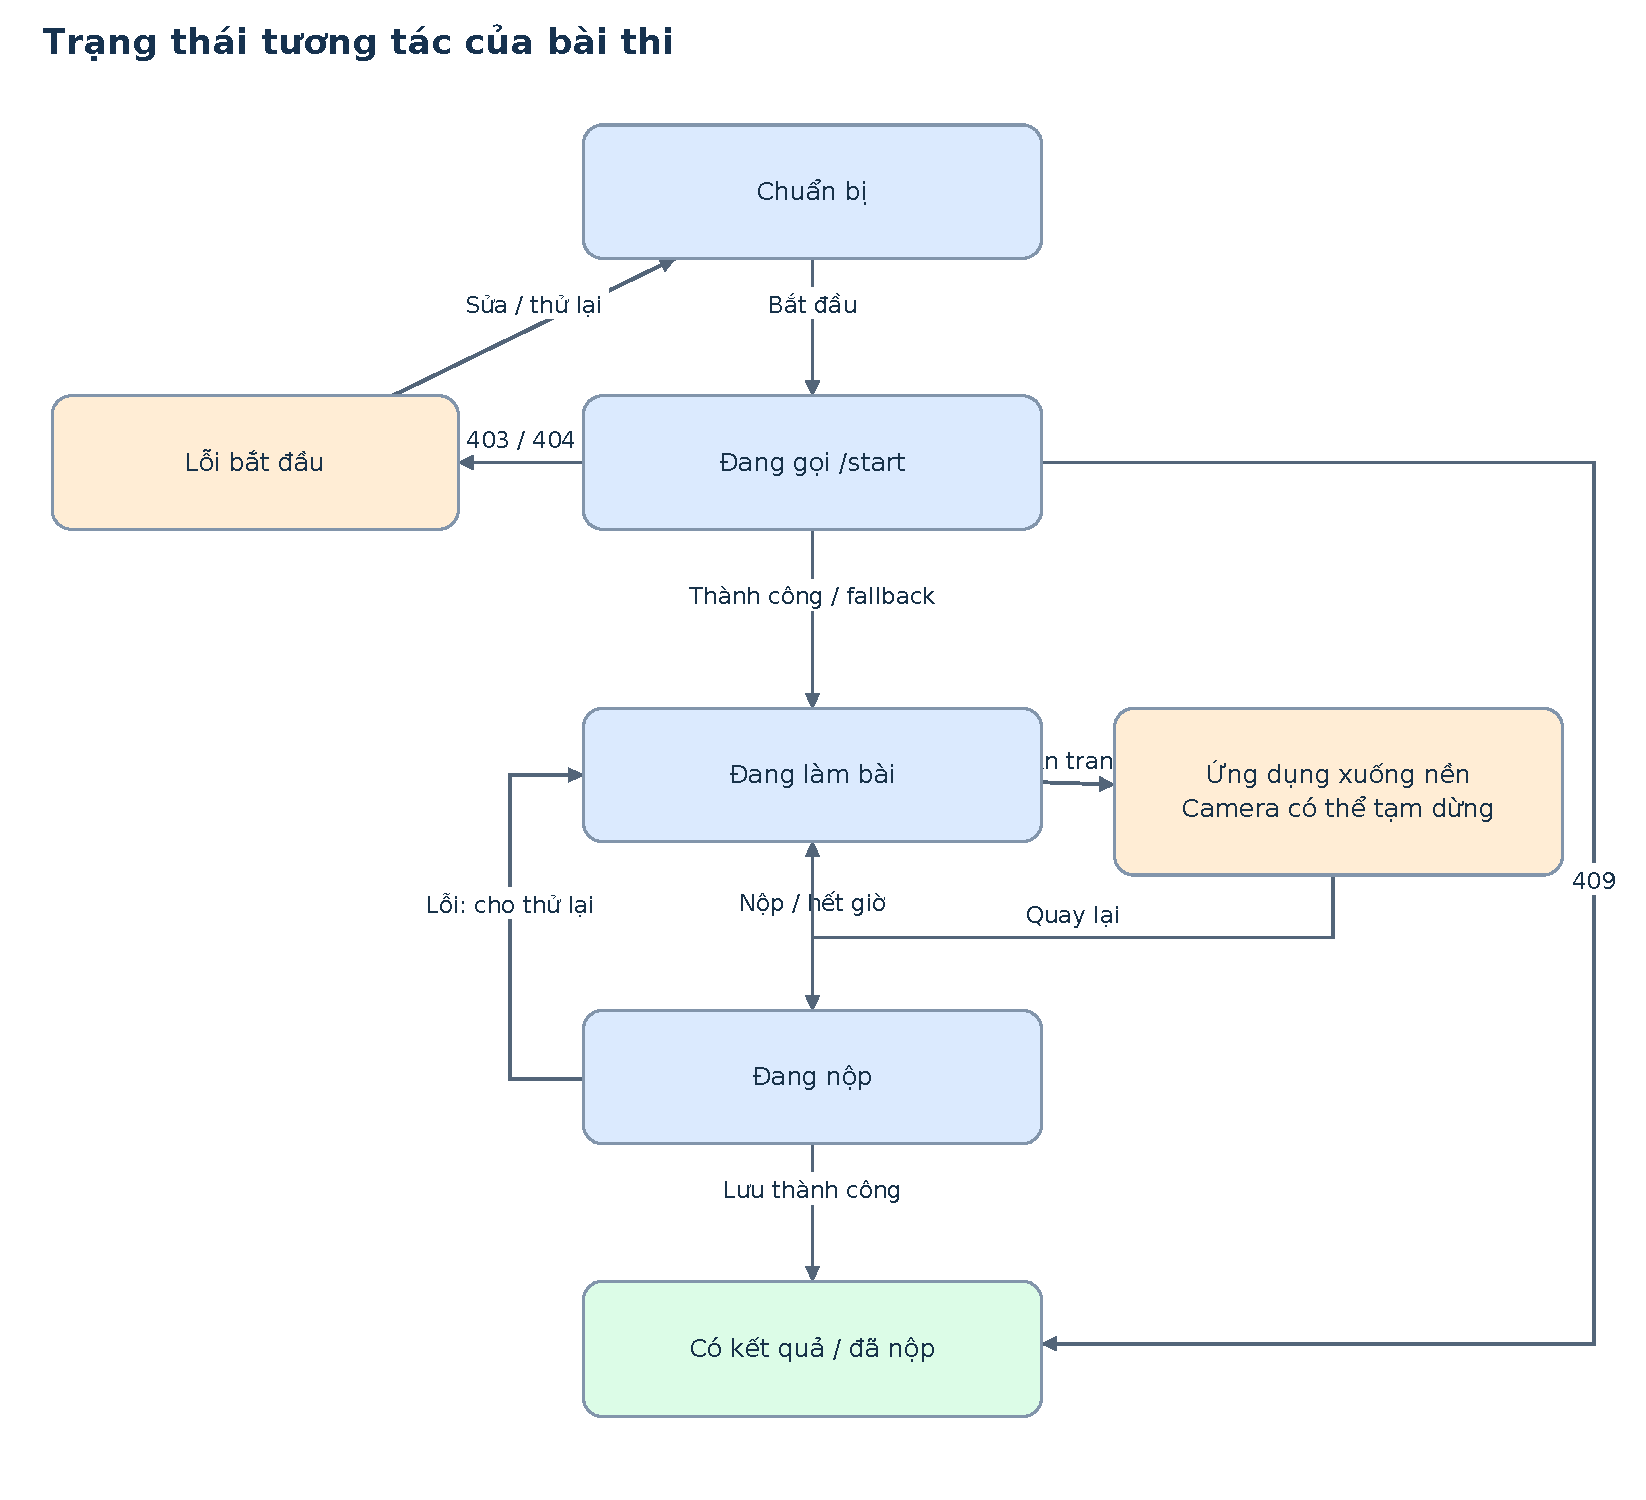
\includegraphics[width=\textwidth,height=0.70\textheight,keepaspectratio]{diagrams/11-state.pdf}
\caption{Trạng thái tương tác của bài thi của EduShield AI.}\label{fig:11-state}
\end{figure}

\clearpage
\subsection{Luồng giám sát AI tại máy khách}
Luồng AI giữ thứ tự ưu tiên nhãn và cooldown. Chu kỳ mobile giảm số lượt suy luận; không suy ra độ chính xác hoặc độ trễ thực đo chỉ từ thông số này.
\begin{figure}[H]
\centering
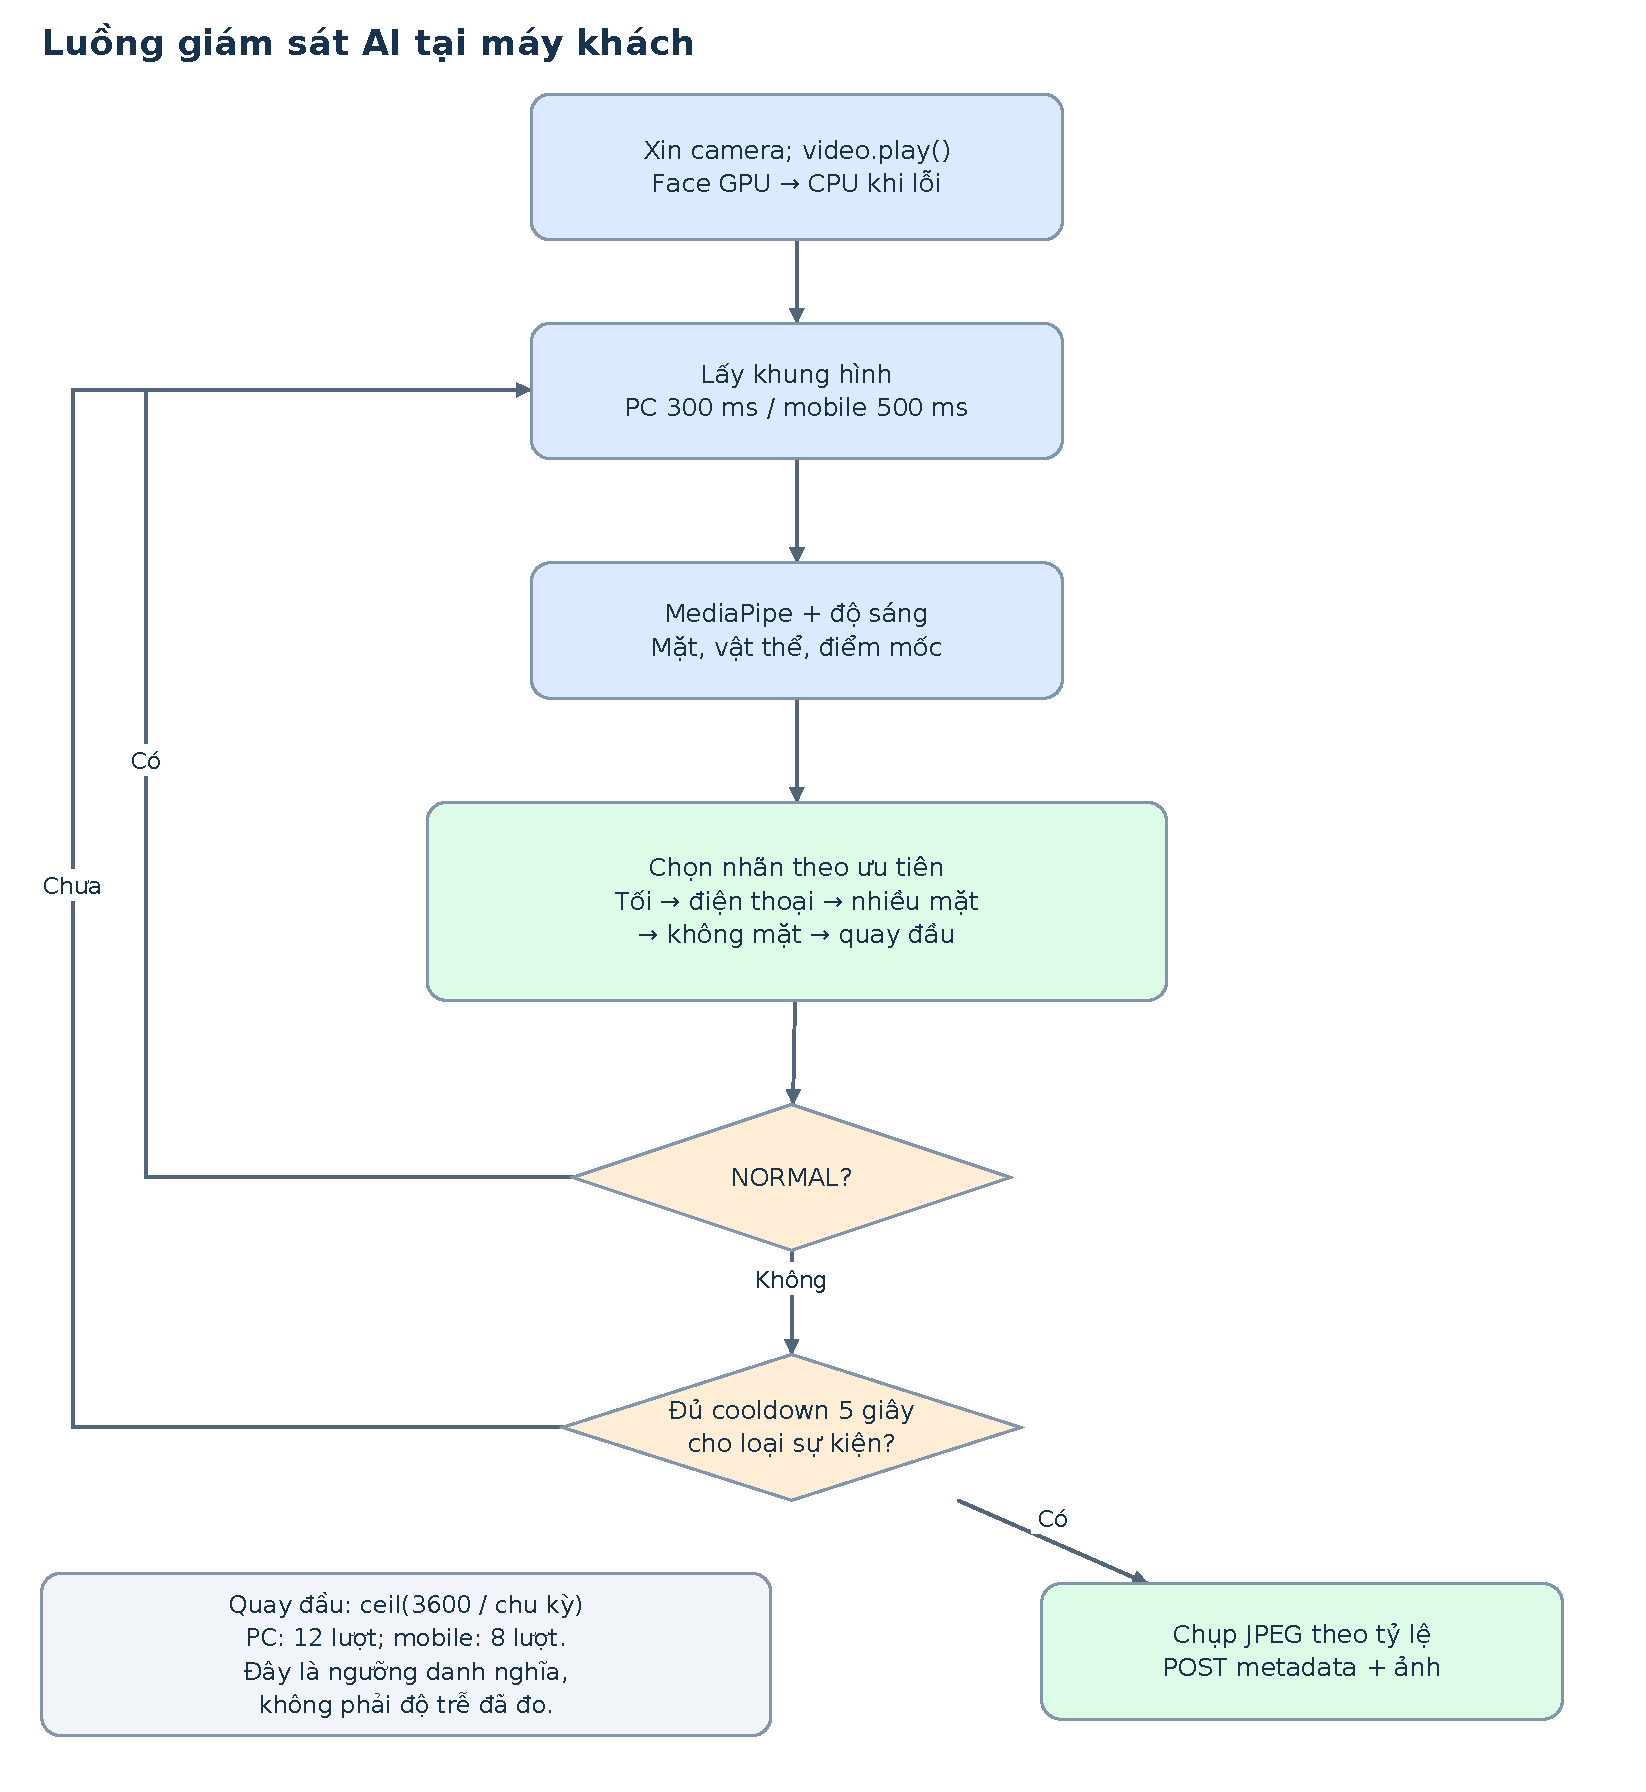
\includegraphics[width=\textwidth,height=0.70\textheight,keepaspectratio]{diagrams/12-ai-flow.pdf}
\caption{Luồng giám sát AI tại máy khách của EduShield AI.}\label{fig:12-ai-flow}
\end{figure}

\chapter{Cài đặt và tích hợp hệ thống}
\markboth{Chương 4. Cài đặt hệ thống}{}
\section{Công nghệ và tổ chức mã nguồn}
Frontend sử dụng React 19, Vite 8, Tailwind CSS 4, MediaPipe Tasks Vision, Framer Motion và Lucide. Backend dùng FastAPI, Uvicorn, SQLAlchemy, APScheduler, python-dotenv, openpyxl, python-docx và python-multipart. Flutter nằm trong thư mục mobile, là phần mở rộng độc lập với frontend web.

Các phụ thuộc JavaScript có package-lock.json; requirements.txt của Python chủ yếu khai báo phiên bản tối thiểu. Vì vậy, môi trường kiểm thử cần lưu phiên bản thực tế đã cài để tái lập. Mô hình được tải từ đường dẫn phiên bản cụ thể, nhưng WASM hiện sử dụng đường dẫn latest; đây là giới hạn đối với tính ổn định khi nguồn ngoài thay đổi.

\section{Tài khoản và phiên truy cập}
\subsection{Giảng viên}
Tài khoản giảng viên được tạo bằng create\_teacher.py. Mã theo định dạng GV-xxxx; mật khẩu được nhập tương tác. auth.py dùng scrypt cùng salt ngẫu nhiên; đường kiểm tra còn hỗ trợ hash PBKDF2 cũ và nâng hash sau đăng nhập thành công. CSDL không lưu mật khẩu dạng rõ.

Đăng nhập thành công tạo token ngẫu nhiên với thời hạn 12 giờ. Máy chủ lưu SHA-256 của token trong teacher\_sessions; frontend giữ token trong sessionStorage và gửi qua Authorization: Bearer. Đăng xuất vô hiệu hóa phiên phía server. Có giới hạn số lần đăng nhập sai theo IP. Cơ chế token legacy chỉ được bật khi cấu hình ALLOW\_LEGACY\_TOKEN=1 và có bí mật tương ứng; đây không phải luồng đăng nhập chính.

\subsection{Sinh viên và phê duyệt}
Mã sinh viên mặc định có dạng SV- theo sau bởi 8 đến 12 chữ số, có thể thay đổi bằng STUDENT\_ID\_REGEX. Sau khi gửi yêu cầu vào thi, sinh viên nhận request token và dùng header X-Request-Token để theo dõi trạng thái. Phê duyệt chưa trực tiếp trả token thi cho giảng viên; lần kiểm tra trạng thái hợp lệ sau đó cấp token thi một lần cho sinh viên. Token được truyền bằng X-Exam-Session ở các yêu cầu lấy đề, bắt đầu, nộp và gửi vi phạm.

Dependency get\_exam\_session kiểm tra bản băm token, trạng thái APPROVED và cờ đã cấp phiên. Backend lấy student\_id, student\_name và exam\_id từ lượt ghi danh. Các schema bài nộp và vi phạm không chấp nhận trường ngoài quy định, giúp tránh việc client tự thay danh tính trong những payload này.

\section{Nhập đề và quản lý lịch}
API upload nhận tên đề, môn học, mã tùy chọn và số phút cho phép xin vào sớm. Tệp giới hạn 5 MiB; bộ đề tối đa 200 câu hợp lệ. Backend đọc worksheet đầu của Excel theo bảy cột, hoặc các đoạn Word theo mẫu câu hỏi--A/B/C/D--đáp án. Dòng thiếu dữ liệu, đáp án sai định dạng và câu trùng được ghi nhận khi phân tích.

Câu trùng được xác định bằng nội dung đã strip và chuyển chữ thường, không phải so khớp ngữ nghĩa. Sau xử lý, thứ tự câu được đánh lại và trọng số mặc định chia đều theo thang 10. Mã đề được chuẩn hóa về ký tự cho phép và kiểm tra duy nhất. Đề mới gắn với tài khoản giảng viên đang đăng nhập.

Công bố yêu cầu thời lượng 1--600 phút, ngưỡng đạt 0--10 và hai mốc mở/đóng hợp lệ. Giao diện cho phép nhập lịch và chuyển thời gian sang dạng gửi API. Sinh viên chỉ truy cập theo điều kiện lịch và phiên của đề. Xáo trộn áp dụng cho thứ tự câu hỏi, không phải hoán đổi các phương án A--D. Thứ tự đã hiển thị có thể được giữ ở tiến độ cục bộ trong phiên trình duyệt.

\section{Mốc bắt đầu, khôi phục và hạn nộp}
Lần bắt đầu đầu tiên tạo exam\_starts với ràng buộc duy nhất theo đề và sinh viên. Gọi lại sử dụng mốc đã có để tính thời gian còn lại; không tạo thời lượng mới. Frontend xác định thời điểm kết thúc cục bộ bằng thời gian còn lại từ server và dùng Date.now() khi cập nhật đồng hồ, thay vì chỉ trừ dần từng giây.

sessionStorage lưu đáp án theo question.id, câu hiện tại, thứ tự câu và thông tin phiên. Khi tải lại, frontend lọc các đáp án còn hợp lệ, phục hồi thứ tự nếu khớp bộ câu và gọi lại API để đồng bộ thời gian. Cơ chế này hỗ trợ tải lại trong phiên trình duyệt, chưa phải lưu nháp trên server hoặc khôi phục từ thiết bị khác.

Đặt $t_s$ là giờ bắt đầu tại server, $D$ là thời lượng tính bằng giây và $t_e$ là giờ đóng đề. Hạn tiếp nhận bài nộp là:
\begin{equation}
 t_{\mathrm{deadline}}=\min(t_s+D+15\text{ giây},\ t_e).
\end{equation}
Khoảng 15 giây dành cho độ trễ gửi bài, không kéo dài giờ đóng đề. API từ chối khi thiếu mốc bắt đầu hoặc giờ server vượt hạn. Cờ auto\_submitted được dùng ghi trạng thái nộp, không thay thế kiểm tra thời gian tại backend.

\section{Chấm bài và xuất kết quả}
Backend truy vấn đáp án chuẩn, tạo ánh xạ lựa chọn theo ID câu và cộng trọng số câu đúng. Điểm được giới hạn tối đa 10 và làm tròn hai chữ số. Bài nộp cùng các câu trả lời được ghi trong giao dịch. Ràng buộc UNIQUE theo đề và sinh viên là lớp cuối chống bản nộp trùng; xung đột được trả về HTTP 409.

Bảng điểm gồm mã, tên sinh viên, điểm, số câu đúng, thời điểm nộp, trạng thái và số vi phạm. Phép đếm vi phạm dùng student\_id cùng exam\_id, không ghép đơn thuần theo khoảng thời gian. Giảng viên có thể xuất bảng điểm Excel. Số vi phạm không được đưa vào công thức trừ điểm.

\section{Khởi tạo camera và mô hình AI}
Camera được yêu cầu với kích thước mong muốn 640$\times$480 và hướng người dùng; độ phân giải thực tế phụ thuộc thiết bị. Face Landmarker chạy VIDEO, tối đa ba khuôn mặt, ngưỡng phát hiện và theo dõi 0,5; ưu tiên GPU rồi thử CPU khi không khởi tạo được. EfficientDet Lite0 chạy CPU, tối đa năm kết quả và ngưỡng 0,25.

Nếu mô hình vật thể tải thất bại, code tiếp tục với phần khuôn mặt và ghi cảnh báo; tính năng phát hiện điện thoại khi đó không hoạt động đầy đủ. Các mô hình được dùng để suy luận từ trọng số có sẵn, không có pipeline huấn luyện trong dự án.

\begin{table}[htbp]\centering
\caption{Thông số AI và ảnh sự kiện trên web}
\begin{tabularx}{\textwidth}{@{}L{6cm}X@{}}\toprule
Thông số & Giá trị \\\midrule
Chu kỳ phân tích & PC 300 ms; điện thoại 500 ms.\\
Khoảng nghỉ cùng nhãn & 5 giây.\\
Điểm điện thoại & Nhãn cell phone, score $>0{,}25$.\\
Landmarks dùng quay đầu & Mũi 1; mắt 133 và 362.\\
Ngưỡng hình học & Độ lệch $>0{,}25$ hoặc bất đối xứng $>1{,}25$.\\
Quay đầu liên tiếp & 12 lượt PC; 8 lượt mobile.\\
Độ sáng & Canvas 64$\times$48; trung bình $<15$.\\
Ảnh bằng chứng & JPEG, rộng 320 px, giữ tỷ lệ, chất lượng 0,6.\\
\bottomrule\end{tabularx}\end{table}

\section{Quy tắc chọn nhãn và gửi sự kiện}
\begin{algorithm}[H]
\caption{Chọn trạng thái giám sát từ một lượt phân tích}
\begin{minipage}{0.94\linewidth}
\small
\textbf{Đầu vào:} khung hình, kết quả mặt/vật thể, bộ đếm $q$, chu kỳ $\Delta t$.\\
\textbf{Đầu ra:} nhãn chính $s$, bộ đếm mới.
\begin{enumerate}[leftmargin=1.6em,itemsep=2pt]
\item Lưu $q_{old}\gets q$ và đặt $q\gets0$.
\item Nếu độ sáng $<15$: chọn CAMERA\_BLOCKED.
\item Ngược lại, nếu có cell phone với score $>0{,}25$: chọn PHONE\_DETECTED.
\item Ngược lại, nếu nhiều hơn một mặt: chọn MULTIPLE\_FACES; nếu không có mặt: chọn NO\_FACE.
\item Với đúng một mặt, tính độ lệch $r$ và bất đối xứng $a$. Nếu $r>0{,}25$ hoặc $a>1{,}25$, đặt $q\gets q_{old}+1$.
\item Riêng nhánh đúng một mặt: chọn TURNING\_HEAD khi $q\geq\lceil3600/\Delta t\rceil$; nếu chưa đủ, chọn NORMAL.
\item Nếu nhãn khác NORMAL và đủ cooldown, gửi sự kiện cùng ảnh.
\end{enumerate}
\end{minipage}
\end{algorithm}

Mỗi lượt chỉ chọn một nhãn theo ưu tiên. Khi điện thoại và nhiều khuôn mặt cùng xuất hiện, nhãn điện thoại được chọn trước. Số bản ghi còn phụ thuộc cooldown, vì vậy không đồng nhất số bản ghi với tổng số hành vi hoặc tổng thời gian vi phạm.
\begin{figure}[H]\centering
\begin{tikzpicture}[x=1cm,y=1cm, every node/.style={font=\fontsize{10}{12}\selectfont}]
\node[rb,font=\fontsize{10}{12}\selectfont] (cam) at (0,0) {Khung hình camera\\300 / 500 ms};
\node[rb,font=\fontsize{10}{12}\selectfont] (face) at (-2.8,-2.4) {Face Landmarker\\Số mặt / landmarks};
\node[rb,font=\fontsize{10}{12}\selectfont] (obj) at (2.8,-2.4) {EfficientDet + Canvas\\Điện thoại / độ sáng};
\node[rb,text width=9cm,font=\fontsize{10}{12}\selectfont] (rule) at (0,-4.8) {Ưu tiên: tối → điện thoại → nhiều mặt\\→ không mặt → quay đầu → bình thường};
\node[rb,font=\fontsize{10}{12}\selectfont] (normal) at (-2.8,-7.2) {NORMAL\\Tiếp tục quan sát};
\node[rb,font=\fontsize{10}{12}\selectfont] (bad) at (2.8,-7.2) {Bất thường\\Kiểm tra cooldown 5 s};
\node[rb,font=\fontsize{10}{12}\selectfont] (send) at (2.8,-9.6) {Ảnh + metadata\\POST với phiên thi};
\draw[ra] (cam)--(face);\draw[ra] (cam)--(obj);\draw[ra] (face)--(rule);\draw[ra] (obj)--(rule);
\draw[ra] (rule)--(normal);\draw[ra] (rule)--(bad);\draw[ra] (bad)--(send);
\end{tikzpicture}

\caption{Luồng xử lý hình ảnh và gửi cảnh báo phía sinh viên.}\end{figure}

Sự kiện trình duyệt đi qua callback riêng. TAB\_SWITCH, WINDOW\_BLUR và FULLSCREEN\_EXIT được gửi khi bài thi hoạt động. Hook gộp các lần rời trang gần nhau trong 1,5 giây; bước gửi áp dụng cooldown theo nhãn. Các thao tác như phím bị chặn hoặc chuột phải có thể chỉ tạo thông báo cục bộ. JavaScript không cung cấp khóa hệ điều hành.

\section{Tiếp nhận sự kiện và bảo vệ lưu trữ}
Backend kiểm tra phiên, loại vi phạm và thời điểm chụp lệch không quá 300 giây so với server. Tần suất được giới hạn 30 sự kiện mỗi phút và 600 sự kiện mỗi lượt ghi danh. Ảnh được giới hạn 300 KB sau giải mã, kiểm tra dấu hiệu JPEG; tổng dung lượng ảnh mặc định 2 GiB, có thể cấu hình bằng biến môi trường.

Tên thư mục sinh viên được chuẩn hóa, tên ảnh có thành phần ngẫu nhiên. Bản ghi lưu đường dẫn ảnh, exam\_id và enrollment\_id; không lưu toàn bộ ảnh nhị phân vào SQLite. Tuyến đọc ảnh yêu cầu phiên giảng viên, không công khai thư mục snapshots.

Nhật ký cục bộ có thể tăng trước khi POST hoàn tất. Code chưa có hàng đợi gửi lại bền vững khi mất mạng, nên số cảnh báo phía sinh viên có thể khác số sự kiện lưu trên server. Các kiểm tra kích thước và kiểu tệp không thay thế đánh giá chất lượng bằng chứng.

\section{CSDL, sao lưu và phục hồi}
Đường dẫn DB được xác định theo thư mục backend, không theo thư mục làm việc của terminal. SQLite sử dụng WAL, synchronous=NORMAL, foreign\_keys=ON và busy\_timeout=5000; thời gian chờ kết nối là 5 giây \cite{sqlitewal}.

Khởi tạo kiểm tra toàn vẹn, tạo các bảng thiếu và chạy migrate\_db. Đây là migration tùy chỉnh theo cấu trúc hiện có, chưa phải hệ thống migration tổng quát có lịch sử phiên bản như Alembic. Backend có cơ chế sao lưu trước cập nhật schema khi cần và sao lưu định kỳ bằng SQLite backup API. Job sao lưu chạy mỗi sáu giờ; cơ chế lưu giữ giữ tối đa bảy bản sao định kỳ theo mẫu tên.

Ảnh được quét mỗi giờ và xóa khi captured\_at cũ hơn 24 giờ; đường dẫn được đặt rỗng, metadata còn lại. Thời hạn thực tế phụ thuộc lúc quét và thời gian dịch vụ hoạt động. captured\_at vẫn do client cung cấp nhưng đã được giới hạn độ lệch khi tiếp nhận.

recover\_db.py đọc nguồn và tạo DB phục hồi mới. Quá trình phục hồi không bảo đảm mọi dữ liệu trong trang hỏng đều còn nguyên. Các thao tác đổi tên/thay DB cần thực hiện khi backend đã dừng. Ngoài ra, handler DatabaseError trả 503 với thông báo thống nhất và rollback session khi có thể.

\section{Giao diện và triển khai đa thiết bị}
Không gian giảng viên gồm quản lý đề, yêu cầu vào thi và giám sát. Dashboard tải lại dữ liệu theo chu kỳ 10 giây; danh sách vi phạm hiện yêu cầu tối đa 500 dòng dù backend có limit/offset. Vì vậy thống kê tổng có thể lớn hơn số dòng đang hiển thị.

Web di động dùng video playsInline, gọi play() rõ ràng, giữ tỷ lệ ảnh và giảm chu kỳ AI xuống 500 ms. Khi chuyển ứng dụng, camera có thể ngừng cung cấp khung hình; hệ thống không tuyên bố quan sát liên tục trong nền. Khi có frontend/dist, FastAPI phục vụ giao diện cùng API và trả SPA fallback cho đường dẫn phù hợp.


Phần Flutter có camera, màn hình thi và các service HTTP. Tuy nhiên, hàm phân loại còn dựa trên chu kỳ thời gian thay vì mô hình AI; phần ước lượng độ sáng xử lý byte ảnh nén chưa đúng như pixel RGB. Service chưa hoàn chỉnh với header phiên thi đã duyệt. Do đó, phạm vi chức năng được đánh giá trong báo cáo tập trung vào backend và web, chưa xác nhận APK/IPA native hoàn chỉnh.
\begin{figure}[H]\centering\begin{tikzpicture}[node distance=0.9cm and 0.7cm]
\node[rb] (pc) {Máy tính\\Web React};
\node[rb,right=of pc] (phone) {Điện thoại\\Chrome / Safari / PWA};
\node[rb,below=of pc] (edge) {Cloudflare\\Địa chỉ HTTPS};
\node[rb,below=of edge] (tunnel) {cloudflared trên laptop\\Chuyển tiếp localhost:8000};
\node[rb,below=of tunnel] (server) {FastAPI\\API + frontend/dist};
\node[rb,right=of server] (store) {SQLite + snapshots\\Bản sao lưu DB};
\draw[ra] (pc)--(edge);\draw[ra] (phone)--(edge);\draw[ra] (edge)--(tunnel);\draw[ra] (tunnel)--(server);\draw[ra] (server)--(store);
\end{tikzpicture}

\caption{Mô hình triển khai web qua HTTPS tunnel.}\end{figure}

\chapter{Kết quả kiểm thử và đánh giá}
\markboth{Chương 5. Kiểm thử và đánh giá}{}
\section{Phạm vi bằng chứng}
Kết quả của chương này gồm hai nguồn: phân tích tĩnh mã nguồn tại commit \texttt{97a11fe} và chạy 17 ca kiểm thử chức năng trên dữ liệu tổng hợp. Tác giả xác nhận các kênh web, APK Android và iOS hoạt động tốt. Lần biên soạn này không trực tiếp thao tác thiết bị thật và không có bộ dữ liệu ảnh gán nhãn hoặc phép đo tải nhiều máy; xác nhận vận hành được tách khỏi kiểm thử tự động. Do đó, những nhận xét về chức năng có mã triển khai được tách khỏi những kết luận đã có bằng chứng chạy thực tế.

Các phép thử được thực hiện bằng Python 3.12.14, FastAPI TestClient, SQLite và các thư viện nhập tệp. Ứng dụng được nạp từ mã nguồn đã tải về; \src{PROCTOR_API_TOKEN} được đặt thành giá trị riêng cho fixture. Thư mục làm việc được chuyển sang một thư mục tạm trước khi khởi tạo CSDL. Không có bài thi hoặc thông tin cá nhân thực được sử dụng.

TestClient trong bộ thử không được mở bằng context manager chạy lifespan, do đó không kiểm thử việc khởi động bộ lập lịch nền. Bộ thử cũng không khởi tạo trình duyệt, webcam hoặc mô hình MediaPipe. Cấu hình này phù hợp kiểm tra bộ phân tích và API nhưng giới hạn rõ ràng điều có thể kết luận.

\section{Dữ liệu và quy trình kiểm thử}
Bộ Excel cơ sở gồm hai câu hỏi với bốn phương án mỗi câu, đáp án đúng lần lượt là A và B. Một biến thể lặp câu đầu để kiểm tra loại trùng; một biến thể thêm câu thiếu phương án; một tệp chứa 201 câu để kiểm tra giới hạn. Bộ Word gồm sáu đoạn văn cho một câu hỏi đúng định dạng.

Luồng API sử dụng mã đề \texttt{DE-TEST} và mã sinh viên giả \texttt{SV-TEST}. Sau khi tạo đề nháp, bộ thử xác nhận sinh viên chưa thể lấy đề. Đề được công bố với thời lượng 10 phút và điểm đạt 5. Sinh viên trả lời A cho cả hai câu, nên kết quả mong đợi là một câu đúng trên hai câu, tương đương 5 điểm. Cuối cùng, bộ thử kiểm tra nộp lặp, xuất Excel và một số hành vi lưu sự kiện.

Kết quả từng phép thử được ghi bằng điều kiện assert tương ứng; nếu một điều kiện sai, chương trình dừng với lỗi. Tệp JSON đi kèm lưu tên ca, trạng thái đạt và nội dung chi tiết khi cần. Cách kiểm thử này không có đo thời gian phản hồi nên báo cáo không đưa ra số liệu mili giây hoặc số yêu cầu mỗi giây.

\section{Kết quả kiểm thử chức năng}
\begin{longtable}{@{}L{1cm}L{5cm}L{7.2cm}L{1.3cm}@{}}
\caption{Kết quả 17 ca kiểm thử đã thực hiện}\label{tab:tests}\\
\toprule Mã & Tình huống & Điều kiện được xác nhận & KQ \\\midrule\endfirsthead
\toprule Mã & Tình huống & Điều kiện được xác nhận & KQ \\\midrule\endhead
P01 & Excel đúng định dạng & Bộ phân tích trả 2 câu hợp lệ. & Đạt\\
P02 & Thêm câu trùng & Số câu hợp lệ vẫn là 2. & Đạt\\
P03 & Thêm câu thiếu lựa chọn & Câu lỗi bị bỏ; còn 2 câu hợp lệ. & Đạt\\
P04 & Tệp có 201 câu & Số câu hợp lệ trả về bằng 0. & Đạt\\
P05 & Word theo mẫu sáu dòng & Bộ phân tích trả 1 câu hợp lệ. & Đạt\\
P06 & Tệp đuôi TXT & Không nhận câu hợp lệ. & Đạt\\
A01 & Lấy danh sách đề thiếu token & HTTP 401. & Đạt\\
A02 & Upload đề hợp lệ có token & HTTP 200 và trạng thái DRAFT. & Đạt\\
A03 & Lấy đề khi còn nháp & HTTP 403. & Đạt\\
A04 & Công bố đề & HTTP 200. & Đạt\\
A05 & Sinh viên lấy đề & HTTP 200; mọi câu đều không chứa correct\_option. & Đạt\\
A06 & Đúng một trong hai câu & HTTP 200; total\_score bằng 5. & Đạt\\
A07 & Nộp lại cùng sinh viên, đề & HTTP 409. & Đạt\\
A08 & Xuất kết quả Excel & Endpoint trả HTTP 200. & Đạt\\
A09 & Sự kiện lúc 14:00 UTC+7 & HTTP 201; thời gian trả về bắt đầu bằng 07:00 UTC cùng ngày. & Đạt\\
A10 & Loại sự kiện UNKNOWN & HTTP 400. & Đạt\\
A11 & Đọc đường dẫn ảnh thiếu token & HTTP 401 trước khi phục vụ ảnh. & Đạt\\
\bottomrule
\end{longtable}

Tổng hợp: \textbf{17/17 ca trong bộ thử đạt}. Đây là tỷ lệ của bộ thử hữu hạn được lựa chọn, không phải độ bao phủ toàn bộ nhánh mã hoặc tỷ lệ lỗi bằng không của hệ thống. Ca A07 là nộp tuần tự, chưa mô phỏng hai yêu cầu thực sự đồng thời. Ca A08 chỉ xác nhận endpoint trả thành công, chưa đối chiếu từng ô trong workbook. Ca A11 dùng đường dẫn ảnh không tồn tại để kiểm tra lớp xác thực đi trước việc phục vụ tệp, chưa xác nhận một ảnh hợp lệ hiển thị thành công trên trình duyệt.

\section{Các kết quả tích cực có căn cứ}
\subsection{Quy trình đề và điểm số}
Các ca P01--P06 cho thấy bộ phân tích hoạt động đúng với một số cấu trúc đầu vào đã chọn, bao gồm dữ liệu lỗi và giới hạn số câu. Chuỗi A02--A06 chứng minh một luồng tạo nháp, chặn lấy sớm, công bố, lấy đề và chấm điểm có thể thực thi qua API. Đáp án đúng không xuất hiện trong phản hồi lấy đề của ca A05.

Việc chấm lại từ câu hỏi trong CSDL thay vì nhận tổng điểm từ trình duyệt là điểm tích cực của thiết kế. Ràng buộc duy nhất trên bản nộp bổ sung một tầng bảo vệ dữ liệu; phép thử nộp lặp xác nhận đường xử lý xung đột tuần tự. Cần bổ sung thử tranh chấp đồng thời để xác nhận hành vi dưới tải và điều kiện khóa SQLite.

\subsection{Truy cập dữ liệu và thời gian}
Các tuyến quản lý và ảnh có kiểm tra token ở backend. Ca A01 và A11 xác nhận hai đường truy cập bị chặn khi thiếu token. Ca A09 xác nhận một thời điểm có độ lệch UTC+7 được chuẩn hóa đúng ở luồng tạo sự kiện. Đây là bằng chứng hẹp nhưng hữu ích cho vấn đề thời gian từng được sửa trong commit khảo sát.

Cơ chế tách metadata và ảnh cho phép giữ lịch sử ngay cả khi ảnh hết hạn. Việc này có lợi cho thống kê, đồng thời đòi hỏi giao diện phân biệt bản ghi còn ảnh và bản ghi chỉ còn thông tin. Khi xem xét một trường hợp, giảng viên cần biết giới hạn của bằng chứng còn lưu.

\section{Các hạn chế và tác động}
\begin{longtable}{@{}L{1cm}L{5.2cm}L{8.3cm}@{}}
\caption{Hạn chế xác định từ mã nguồn và mức ưu tiên xử lý}\\
\toprule Mã & Hạn chế & Tác động và hướng xử lý \\\midrule\endfirsthead
\toprule Mã & Hạn chế & Tác động và hướng xử lý \\\midrule\endhead
H01 & Mã sinh viên tự khai; chưa có phiên xác thực cá nhân. & Có thể gán dữ liệu cho mã khác. Ưu tiên bổ sung tài khoản hoặc vé vào thi do máy chủ cấp.\\
H02 & Timer và cờ tự nộp phụ thuộc máy khách; đã lưu bắt đầu nhưng submit chưa cưỡng chế deadline. & Không bảo đảm hạn nộp. Cần kiểm tra mốc bắt đầu, deadline tại API nộp và hạn chế fallback cấp lại giờ.\\
H03 & Sự kiện không có exam\_id/session\_id. & Có thể cộng nhầm sự kiện giữa các bài thi. Cần liên kết khóa ngoại với phiên thi.\\
H04 & Chuyển tab đã có đường gửi server; gửi lỗi chưa retry bền vững. & Cần kiểm thử đầu cuối trên thiết bị và khi chuyển ứng dụng/mất mạng.\\
H05 & Gửi sự kiện chưa có hàng đợi bền vững. & Mất mạng có thể mất bản ghi. Cần định danh sự kiện, retry có kiểm soát và chống ghi trùng.\\
H06 & Ngưỡng hình học, độ sáng chưa hiệu chuẩn. & Báo nhầm hoặc bỏ sót theo thiết bị, ánh sáng, tư thế. Cần dữ liệu đánh giá và chọn ngưỡng độc lập.\\
H07 & Token giảng viên dùng chung, có thể sinh và ghi log. & Khó phân quyền, quy trách nhiệm và thu hồi riêng. Cần quản lý tài khoản, phiên và bí mật phù hợp.\\
H08 & Tuổi ảnh dựa trên thời gian máy khách. & Chính sách lưu có thể lệch. Cần mốc tiếp nhận phía máy chủ và kiểm tra độ lệch.\\
H09 & Vòng đời camera/timer sau nộp cần kiểm chứng. & Có thể tiếp tục dùng tài nguyên hoặc ghi sự kiện sau bài thi. Cần điều kiện kết thúc và kiểm thử trình duyệt.\\
H10 & Không có migration CSDL có phiên bản. & Cập nhật mô hình có thể không nâng bảng cũ. Cần kế hoạch migration và kiểm thử khôi phục.\\
H11 & Tài nguyên WASM dùng đường dẫn latest. & Khó tái lập và có thể lệch phiên bản gói. Cần khóa phiên bản hoặc tự phục vụ tài nguyên.\\
H12 & Danh sách giới hạn và thống kê tổng khác phạm vi. & Người dùng có thể hiểu nhầm số liệu. Cần phân trang rõ và thông báo bộ lọc đang áp dụng.\\
\bottomrule
\end{longtable}

Đây là các giới hạn cần ưu tiên theo mục đích sử dụng, không phải khẳng định đã có sự cố khai thác trong thực tế. Với một buổi trình diễn đồ án, có thể kiểm soát môi trường và giải thích giới hạn. Với kỳ thi có hậu quả học vụ, cần hoàn thiện định danh, phiên thi, giao nhận sự kiện và quy trình con người xem xét trước khi dựa vào dữ liệu để ra quyết định.

\section{Kế hoạch thực nghiệm AI đề xuất}
\subsection{Thiết kế bộ dữ liệu}
Nên thu các đoạn video ngắn có sự đồng ý của người tham gia, gồm trạng thái bình thường và từng tình huống: rời khung hình, thêm người, đưa điện thoại vào vùng nhìn, quay đầu và che camera. Mỗi loại cần nhiều điều kiện ánh sáng, khoảng cách, góc đặt máy và thiết bị. Cần có các trường hợp khó như cầm vật giống điện thoại, quay đầu ngắn để nghe âm thanh hoặc phòng tối nhưng không che camera.

Đơn vị dữ liệu nên là đoạn hoặc khoảng sự kiện, có thời điểm bắt đầu và kết thúc được người gán nhãn xác nhận. Không chia ngẫu nhiên các khung hình liền kề của cùng một video vào cả tập hiệu chỉnh và tập kiểm tra vì sẽ tạo tương đồng quá lớn. Nên tách theo người hoặc phiên quay để đánh giá khả năng hoạt động trên trường hợp chưa thấy.

Ngưỡng cần được hiệu chỉnh trên một tập riêng, sau đó cố định trước khi chạy tập kiểm tra. Do dự án dùng mô hình có sẵn, bước này là hiệu chỉnh hệ thống quyết định, không nên gọi là huấn luyện lại mạng nếu không thực hiện cập nhật trọng số.

\subsection{Chỉ số và bảng ghi kết quả}
Cần báo cáo precision, recall và F1 theo từng loại; số cảnh báo nhầm mỗi giờ trong phiên bình thường; độ trễ từ lúc sự kiện bắt đầu đến lần ghi đầu tiên. Với thứ tự ưu tiên hiện tại, cần thêm nhóm tình huống nhiều dấu hiệu đồng thời để quan sát nhãn bị che. Các mẫu số bằng không phải được xử lý minh bạch, không tự thay bằng điểm hoàn hảo.

\begin{table}[htbp]
\centering
\caption{Biểu mẫu thực nghiệm AI -- chưa có số liệu đo}
\begin{tabularx}{\textwidth}{@{}Xcccc@{}}\toprule
Loại & Precision & Recall & F1 & Trễ p95 \\\midrule
Không có mặt & -- & -- & -- & --\\
Nhiều khuôn mặt & -- & -- & -- & --\\
Điện thoại & -- & -- & -- & --\\
Quay đầu & -- & -- & -- & --\\
Khung hình tối & -- & -- & -- & --\\\bottomrule
\end{tabularx}
\end{table}

Dấu ``--'' thể hiện chưa đo, không phải giá trị bằng 0. Khi điền bảng cần kèm số mẫu, thiết bị, phiên bản mô hình, cách ghép cảnh báo với khoảng nhãn chuẩn và quy tắc chấp nhận độ trễ. Nếu chỉ báo một tỷ lệ tổng, số lượng khung hình bình thường lớn có thể che khuất khả năng bỏ sót các sự kiện hiếm.

\section{Kế hoạch kiểm thử tích hợp và hiệu năng}
Các ca tích hợp tiếp theo nên bao gồm cấp/từ chối quyền camera, mất mạng rồi kết nối lại, CDN mô hình không tải được, nộp bài khi gần hết giờ, rời trang trong lúc gửi bài, nhận kết quả rồi xác nhận camera đã dừng. Cần quan sát cả màn hình sinh viên, dữ liệu máy chủ và màn hình giảng viên để phát hiện sai lệch giữa các tầng.

Về tải, có thể tăng dần số máy khách giả lập cho các API đọc và ghi, ghi nhận p50/p95 thời gian phản hồi, tỷ lệ lỗi, thời gian chờ khóa và kích thước CSDL. Suy luận AI chạy trên thiết bị sinh viên nên thử tải HTTP không phản ánh được độ mượt camera; phần này phải đo trên thiết bị mục tiêu. Không đưa ra cam kết số sinh viên đồng thời trước khi có cấu hình phần cứng, kịch bản và kết quả.

Về giao diện, cần kiểm tra câu hỏi và phương án dài, màn hình nhỏ, mức phóng đại chữ và vị trí hộp cảnh báo. Tiêu chí nghiệm thu nên cụ thể: người dùng thấy trạng thái camera và điều khiển chính; nội dung không bị cắt; khu vực cuộn rõ ràng; focus bàn phím không bị mắc trong hộp thoại. Các thử nghiệm này chưa được thực hiện trong bộ 17 ca backend.

\section{Riêng tư, công bằng và vai trò giảng viên}
Ảnh khuôn mặt và lịch sử hành vi là dữ liệu có thể gây ảnh hưởng đến người học. Hệ thống cần thông báo rõ mục đích, loại dữ liệu, người được xem và thời hạn lưu trước khi bắt đầu. Cơ chế dọn ảnh là một thành phần kỹ thuật của quản lý dữ liệu, không tự bảo đảm đầy đủ quy trình tổ chức hoặc tuân thủ pháp lý.

Các điều kiện ánh sáng, camera, kính, tư thế và đặc điểm cá nhân có thể làm chất lượng nhận diện khác nhau. Thực nghiệm nên ghi nhận các yếu tố liên quan mà không thu thập thông tin nhạy cảm vượt quá nhu cầu. Cần có cách xử lý khi thiết bị không đáp ứng hoặc cảnh báo bị đánh giá sai, thay vì tự động trừ điểm dựa trên nhãn AI.

Báo cáo đề xuất xem mỗi sự kiện là một yêu cầu xem xét. Giảng viên đối chiếu ảnh, thời gian, bối cảnh và phản hồi của sinh viên trước khi kết luận. Điểm học tập do đáp án trắc nghiệm quyết định; mã nguồn hiện tại không thể hiện cơ chế tự động khấu trừ điểm theo số cảnh báo, và báo cáo không bổ sung một quy chế như vậy.

\section{Kiểm chứng phần mở rộng đa thiết bị ngày 01/10/2026}
Bộ 17 ca cũ được chạy lại với commit \texttt{97a11fe} và đều đạt. Bổ sung 11 ca API tập trung vào mốc bắt đầu, tiếp tục thời gian, dữ liệu nộp và sự kiện trình duyệt; cả 11 ca đạt điều kiện kiểm tra. Kết quả tại \src{evidence/results-current.json} và \src{evidence/results-mobile.json}. Hai ca xác nhận giới hạn hiện hữu có kết quả ``đạt'' nghĩa là tái hiện đúng hành vi, không có nghĩa hệ thống đã đáp ứng yêu cầu cưỡng chế thời gian.
\begin{longtable}{@{}L{1cm}L{10.7cm}L{2.9cm}@{}}
\caption{Kiểm thử API bổ sung cho bản đa thiết bị}\\
\toprule Mã & Hành vi / điều kiện kiểm tra & Kết quả \\\midrule\endfirsthead
\toprule Mã & Hành vi / điều kiện kiểm tra & Kết quả \\\midrule\endhead
M01 & start từ chối đề nháp (403). & Đạt\\
M02 & Lần bắt đầu đầu tiên trả mốc UTC và thời gian gần đủ. & Đạt\\
M03 & Gọi lại giữ mốc cũ, chỉ một hàng exam\_starts. & Đạt\\
M04 & Mốc bắt đầu lùi 120 giây làm giảm thời gian còn lại tương ứng. & Đạt\\
M05 & Đã quá thời lượng thì remaining\_seconds bằng 0. & Đạt\\
M06 & Xác nhận giới hạn: submit vẫn nhận bài đã quá thời lượng. & Tái hiện\\
M07 & started\_at được sao chép từ exam\_starts vào bài nộp. & Đạt\\
M08 & Đã nộp thì gọi start trả 409. & Đạt\\
M09 & Backend nhận TAB\_SWITCH không kèm ảnh (201). & Đạt\\
M10 & Mã đề không tồn tại trả 404. & Đạt\\
M11 & Xác nhận giới hạn: có thể submit không gọi start trước. & Tái hiện\\
\bottomrule
\end{longtable}
Các phép thử dùng SQLite tạm và dữ liệu tổng hợp; không sửa dữ liệu vận hành. Chúng không đo camera, WebView APK, Safari, Cloudflare Tunnel hoặc khả năng chịu tải. Kết quả M09 xác nhận API nhận nhãn, không thay thế thao tác chuyển ứng dụng trên điện thoại thật.

\subsection{Ma trận nghiệm thu trên thiết bị thật}
Tác giả xác nhận hệ thống hoạt động tốt trên các kênh đã triển khai. Để biến xác nhận này thành hồ sơ nghiệm thu có thể tái lập, cần ghi model thiết bị, phiên bản OS/trình duyệt hoặc APK, ngày chạy, đường dẫn build và kết quả từng bước. Các mục dưới đây là danh sách kiểm tra bổ sung, không gán số liệu chưa đo.
\begin{longtable}{@{}L{3cm}L{8.2cm}L{3.4cm}@{}}
\toprule Nhóm & Thao tác và tiêu chí & Bằng chứng cần bổ sung \\\midrule
Web PC & Mở tunnel, làm bài, nộp và đối chiếu điểm trên web giảng viên. & OS, browser, ảnh kết quả.\\
Android web/PWA & Cấp camera, tải AI, nhập liệu, cuộn và cảnh báo trên màn hình nhỏ. & Máy, OS, Chrome, video.\\
Android APK & Cài gói, kiểm tra API base, camera và đồng bộ nhật ký/điểm. & APK version, commit native.\\
iOS Safari/PWA & Camera hiển thị, AI sẵn sàng, có thể hoàn thành bài qua link HTTPS. & Máy, iOS, Safari, video.\\
Chuyển ứng dụng & Rời và quay lại; đối chiếu nhật ký SV/GV, thời gian còn lại. & Thời điểm, loại sự kiện, ảnh.\\
Tải lại / mất mạng & Kiểm tra giữ mốc giờ, mất lựa chọn và fallback; mô tả lỗi trung thực. & Yêu cầu, phản hồi, log.\\
Vòng đời & Nộp bài, rời màn hình, kiểm tra camera, timer và sự kiện nền. & Video/nhật ký tài nguyên.\\
\bottomrule
\end{longtable}

\chapter{Kết luận và hướng phát triển}
\section{Kết quả đạt được}
EduShield AI đã tích hợp quy trình thi trắc nghiệm từ tài khoản giảng viên, nhập đề, công bố lịch, phê duyệt sinh viên đến làm bài, chấm điểm và xuất kết quả. Phiên thi được cấp theo lượt ghi danh, giúp ràng buộc quyền tham gia và xác định danh tính dùng trong nghiệp vụ sau phê duyệt.

Mốc bắt đầu lưu tại máy chủ và điều kiện hạn nộp bảo vệ thời gian làm bài; ràng buộc duy nhất ngăn bản nộp trùng. Vi phạm được gắn với đề và lượt ghi danh, hỗ trợ truy vết và thống kê theo đúng bài thi. Hệ thống có dọn ảnh, sao lưu, kiểm tra toàn vẹn và công cụ phục hồi dữ liệu.

Phần AI tích hợp Face Landmarker và EfficientDet Lite0 ngay trong trình duyệt. Các quy tắc hình học, độ sáng, ưu tiên nhãn và cooldown biến đầu ra mô hình thành cảnh báo có thể tra cứu. Giá trị của đề tài nằm ở tổ chức hệ thống quanh các mô hình có sẵn; không phải phát triển một mạng nơ-ron mới.

Kiểm thử chức năng trên dữ liệu tổng hợp cung cấp bằng chứng cho những đường xử lý được mô tả ở chương 5. Các kết quả này không thay thế kiểm thử camera trên thiết bị thật hoặc đo độ chính xác nhận diện. Web di động dùng chung frontend; ứng dụng Flutter còn cần hoàn thiện trước khi được xem là một kênh thi tương đương.

\section{Những vấn đề còn tồn tại}
Danh tính sinh viên vẫn do người dùng khai báo, chưa đối chiếu với hồ sơ đào tạo hoặc nhận diện sinh trắc học. Nhãn cảnh báo được tạo tại client, chưa có cơ chế bảo đảm tín hiệu không bị sửa đổi. Hệ thống chưa có hàng đợi sự kiện bền vững khi mất mạng hoặc lưu nháp câu trả lời trên server.

Ngưỡng AI chưa được hiệu chuẩn bằng bộ dữ liệu độc lập. Một nhãn ưu tiên có thể che dấu hiệu khác trong cùng khung hình. Vòng đời camera/timer sau nộp, độ ổn định trên trình duyệt di động và khả năng chịu tải vẫn cần thử nghiệm bổ sung. Phân quyền theo lớp, quy trình xét duyệt cảnh báo và nhật ký truy cập chưa hoàn chỉnh.

\section{Hướng phát triển}
\begin{longtable}{@{}L{1.3cm}L{6.2cm}L{7.1cm}@{}}
\caption{Các hướng phát triển tiếp theo}\\
\toprule Ưu tiên & Nội dung & Tiêu chí đánh giá \\\midrule\endhead
1 & Xác minh danh tính theo danh sách lớp; kiểm tra phân quyền nhất quán; hoàn thiện kết thúc phiên và camera. & Phiên đúng đối tượng; dữ liệu đúng phạm vi; tài nguyên dừng sau nộp.\\
2 & Lưu nháp server; hàng đợi sự kiện có retry và ID chống trùng; cải thiện phục hồi khi phản hồi cấp phiên bị mất. & Khôi phục theo chính sách; không mất hoặc nhân đôi dữ liệu ngoài dự kiến.\\
3 & Thu dữ liệu có nhãn, hiệu chỉnh ngưỡng và đo hiệu năng thiết bị. & Precision, recall, F1, cảnh báo nhầm/giờ và độ trễ theo từng nhãn.\\
4 & Đồng bộ Flutter với phiên thi; thay phân loại mô phỏng bằng mô hình phù hợp. & Luồng đầu cuối trên thiết bị thật và bằng chứng nhận diện.\\
5 & Hoàn thiện migration có phiên bản, kiểm thử tải và quy trình khôi phục. & Tái lập môi trường, nâng cấp dữ liệu và đo giới hạn trên cấu hình xác định.\\
\bottomrule
\end{longtable}


\backmatter
\cleardoublepage\phantomsection
\addcontentsline{toc}{chapter}{Tài liệu tham khảo}
\bibliographystyle{plain}
\bibliography{refs}
\chapter*{Phụ lục A. Danh mục API}
\markboth{Phụ lục A. Danh mục API}{}
\setcounter{table}{0}\renewcommand{\thetable}{A.\arabic{table}}
\renewcommand{\theHtable}{appendixA.\arabic{table}}
\setcounter{lstlisting}{0}\renewcommand{\thelstlisting}{A.\arabic{lstlisting}}
\addcontentsline{toc}{chapter}{Phụ lục A. Danh mục API}
Danh mục dưới đây được đối chiếu với các decorator trong \src{main.py} và \src{exams_router.py}. ``GV'' nghĩa là cần token giám thị; ``Công khai'' nghĩa là không yêu cầu token giám thị, không đồng nghĩa với việc có xác thực sinh viên riêng. Các API tài liệu tự sinh của framework không nằm trong danh mục nghiệp vụ.

\begin{longtable}{@{}L{1.9cm}L{6.9cm}L{1.8cm}L{3.9cm}@{}}
\caption{Các tuyến API nghiệp vụ và tình trạng truy cập}\\
\toprule Phương thức & Đường dẫn & Quyền & Chức năng \\\midrule\endfirsthead
\toprule Phương thức & Đường dẫn & Quyền & Chức năng \\\midrule\endhead
POST & \src{/api/violations} & Công khai & Tạo sự kiện, có thể kèm ảnh.\\
GET & \src{/api/violations} & GV & Danh sách, bộ lọc, limit/offset.\\
GET & \src{/api/students} & GV & Tổng hợp theo sinh viên.\\
GET & \src{/api/violations/stats} & GV & Thống kê sự kiện.\\
DELETE & \src{/api/violations/all} & GV & Xóa toàn bộ sự kiện và dữ liệu ảnh liên quan.\\
DELETE & \src{/api/violations/{violation_id}/image} & GV & Xóa ảnh của một sự kiện.\\
GET & \src{/api/snapshots/{student_folder}/{filename}} & GV & Đọc ảnh minh chứng.\\
GET & \src{/health} & Công khai & Kiểm tra trạng thái dịch vụ.\\
POST & \src{/api/exams/upload} & GV & Nhập tệp, tạo đề nháp.\\
GET & \src{/api/exams} & GV & Danh sách đề.\\
GET & \src{/api/exams/{exam_id}} & GV & Chi tiết có đáp án.\\
POST & \src{/api/exams/{exam_id}/publish} & GV & Công bố và cấu hình đề.\\
DELETE & \src{/api/exams/{exam_id}} & GV & Xóa đề chưa có bài nộp.\\
GET & \src{/api/exams/code/{exam_code}/take} & Công khai & Lấy đề không kèm đáp án.\\
POST & \src{/api/exams/code/{exam_code}/start} & Công khai & Ghi mốc bắt đầu, trả thời gian còn lại.\\
POST & \src{/api/exams/code/{exam_code}/submit} & Công khai & Nộp và chấm bài.\\
GET & \src{/api/exams/{exam_id}/results} & GV & Kết quả theo đề.\\
GET & \src{/api/exams/{exam_id}/export} & GV & Xuất bảng điểm Excel.\\
\bottomrule
\end{longtable}

\section*{A.1. Ví dụ yêu cầu nộp bài}
Ví dụ sử dụng ID câu hỏi giả định 101 và 102. Khi chạy thực tế phải lấy ID từ phản hồi API lấy đề; không sao chép nguyên ID minh họa.
\begin{lstlisting}[language={},caption={Cấu trúc JSON nộp bài minh họa}]
{
  "student_id": "SV-DEMO",
  "student_name": "Demo Student",
  "answers": [
    {"question_id": 101, "selected_option": "A"},
    {"question_id": 102, "selected_option": "B"}
  ],
  "auto_submitted": false
}
\end{lstlisting}
Phản hồi thành công gồm \src{total_score}, \src{correct_count}, \src{total_questions}, \src{pass_score}, \src{passed}, \src{status}. Mã 409 biểu thị sinh viên đã có bản nộp cho đề. Ứng dụng cần xử lý tình huống máy chủ đã lưu nhưng phản hồi bị mất: gửi lại có thể nhận 409, nên nên có tuyến tra cứu xác nhận bản nộp theo phiên ở phiên bản tiếp theo.

\section*{A.2. Ví dụ yêu cầu ghi sự kiện}
\begin{lstlisting}[language={},caption={Sự kiện minh họa không kèm ảnh}]
{
  "student_id": "SV-DEMO",
  "student_name": "Demo Student",
  "violation_type": "NO_FACE",
  "captured_at": "2026-09-25T14:00:00+07:00"
}
\end{lstlisting}
Ảnh khi có được truyền qua \src{image_base64}. Backend chấp nhận năm nhãn camera và ba nhãn trình duyệt: \src{TAB_SWITCH}, \src{WINDOW_BLUR}, \src{FULLSCREEN_EXIT}. Sự chấp nhận ở API không chứng minh frontend hiện đã gửi ba nhãn này.

\chapter*{Phụ lục B. Hướng dẫn sử dụng và vận hành}
\markboth{Phụ lục B. Hướng dẫn vận hành}{}
\setcounter{table}{0}\renewcommand{\thetable}{B.\arabic{table}}
\renewcommand{\theHtable}{appendixB.\arabic{table}}
\setcounter{lstlisting}{0}\renewcommand{\thelstlisting}{B.\arabic{lstlisting}}
\addcontentsline{toc}{chapter}{Phụ lục B. Hướng dẫn sử dụng và vận hành}
\section*{B.1. Chuẩn bị môi trường phát triển}
Cần Git, Python phù hợp với các phụ thuộc và Node.js đáp ứng yêu cầu của phiên bản Vite trong lockfile. Bộ kiểm thử của báo cáo chạy trên Python 3.12.14. Nên dùng môi trường ảo riêng, cài từ tệp dự án và ghi lại phiên bản thực tế. Các lệnh dưới đây minh họa môi trường Bash.

\begin{lstlisting}[language=bash,caption={Lấy đúng phiên bản mã khảo sát}]
git clone https://github.com/GBinh02/AI-Protoring.git
cd AI-Protoring
git checkout 97a11fea3ed322e3c05eec84a3ff43acea11e51e
cd backend
python -m venv .venv
source .venv/bin/activate
python -m pip install -r requirements.txt
\end{lstlisting}
Trên Windows PowerShell, lệnh kích hoạt môi trường tương ứng là \src{.venv/Scripts/Activate.ps1}. Không cần đổi chính sách máy nếu môi trường hiện tại đã cho phép chạy; có thể gọi trực tiếp Python trong môi trường ảo theo cấu hình của người dùng.

Đặt \src{PROCTOR_API_TOKEN} bằng một giá trị bí mật riêng trước khi khởi động. Giá trị \texttt{report-fixture-only} trong mã kiểm thử chỉ dành cho dữ liệu giả lập, không dùng làm token vận hành. Không đưa token thật vào báo cáo, kho mã công khai hoặc tệp ảnh chụp màn hình.

\begin{lstlisting}[language=bash,caption={Chạy backend và frontend trong hai terminal}]
# Terminal 1: thu muc backend, da cau hinh token
uvicorn main:app --host 127.0.0.1 --port 8000 --reload

# Terminal 2: thu muc frontend
npm ci
npm run dev
\end{lstlisting}
Kiểm tra \src{http://127.0.0.1:8000/health} để xác nhận backend phản hồi; mở địa chỉ frontend do Vite in ra. Proxy \src{/api} được cấu hình trỏ đến localhost:8000. Nếu thay cổng backend, cần chỉnh cấu hình tương ứng. Hướng dẫn này được suy ra từ cấu trúc dự án; bộ kiểm thử báo cáo không khởi chạy hai tiến trình web để thử camera.

\section*{B.2. Quy trình của giảng viên}
\begin{enumerate}
\item Truy cập vai trò giảng viên và cung cấp token được quản trị viên cấu hình.
\item Mở quản lý đề, chuẩn bị tệp đúng mẫu và tải lên; đọc số câu chấp nhận cùng danh sách lỗi.
\item Kiểm tra nội dung và đáp án, cấu hình thời lượng, điểm đạt và xáo trộn; công bố khi đã sẵn sàng.
\item Cung cấp mã đề cho sinh viên. Trước buổi thi, thử luồng với dữ liệu giả và thiết bị mục tiêu.
\item Theo dõi tổng quan, lọc sinh viên và đọc ảnh cùng thời gian khi có cảnh báo. Chờ chu kỳ cập nhật hoặc tải lại khi cần.
\item Xem kết quả và xuất Excel. Kiểm tra phạm vi sự kiện được ghép vào điểm số, nhất là khi một mã sinh viên làm nhiều đề.
\end{enumerate}
Các thao tác xóa dữ liệu cần được cân nhắc theo quy trình lưu trữ của lớp học. API xóa đề từ chối khi đã có bài nộp, nhưng các API xóa sự kiện vẫn là thao tác riêng; không sử dụng chúng để thử nghiệm trên dữ liệu cần giữ.

\section*{B.3. Quy trình của sinh viên}
\begin{enumerate}
\item Nhập chính xác thông tin theo hướng dẫn của giảng viên và mã đề được cung cấp.
\item Chuẩn bị camera, vị trí ngồi, ánh sáng và kết nối mạng; đóng các ứng dụng không cần thiết.
\item Cho phép camera khi được hỏi và chờ trạng thái mô hình. Báo giảng viên nếu thiết bị không thể khởi tạo.
\item Đọc câu hỏi, chọn đáp án và theo dõi thời gian; kiểm tra các câu chưa trả lời trước khi nộp.
\item Nộp bài, chờ phản hồi xác nhận. Khi có lỗi mạng, không suy đoán rằng thao tác đã thành công chỉ vì đã nhấn nút.
\item Sau khi hoàn tất, rời màn hình thi và kiểm tra chỉ báo camera trên trình duyệt đã tắt.
\end{enumerate}
Cảnh báo có thể xuất hiện do điều kiện môi trường hoặc nhận diện sai. Sinh viên cần có kênh phản hồi và giảng viên cần xem xét trước khi đưa ra quyết định liên quan kết quả học tập.

\section*{B.4. Lưu trữ, sao lưu và triển khai}
CSDL SQLite và thư mục snapshots cần được quản lý cùng nhau vì CSDL chứa đường dẫn tới tệp ảnh. Khi sao lưu một CSDL đang bật WAL, nên dùng cơ chế sao lưu nhất quán của SQLite hoặc dừng ghi theo quy trình phù hợp, không tùy tiện chỉ sao chép tệp chính trong lúc đang thay đổi dữ liệu.

Bản build frontend được tạo bằng \src{npm run build}. Đưa thư mục build lên máy phục vụ tĩnh và cấu hình chuyển tiếp API tới backend; bổ sung HTTPS cho môi trường công khai. Chỉ cấu hình CORS không thay thế xác thực. Giá trị cho phép origin rộng trong mã cần được rà soát theo miền triển khai thực tế.

Khi chạy nhiều tiến trình backend, cần xác định một nơi chịu trách nhiệm tác vụ dọn ảnh để tránh nhiều scheduler cùng thao tác. Trước khi nâng phiên bản, sao lưu dữ liệu, chạy kiểm thử và chuẩn bị migration nếu mô hình bảng thay đổi. Các công việc này là hướng dẫn triển khai đề xuất, chưa phải một pipeline vận hành đã có trong kho.

\chapter*{Phụ lục C. Định dạng đề thi}
\markboth{Phụ lục C. Định dạng đề thi}{}
\setcounter{table}{0}\renewcommand{\thetable}{C.\arabic{table}}
\renewcommand{\theHtable}{appendixC.\arabic{table}}
\setcounter{lstlisting}{0}\renewcommand{\thelstlisting}{C.\arabic{lstlisting}}
\addcontentsline{toc}{chapter}{Phụ lục C. Định dạng đề thi}
\section*{C.1. Mẫu Excel}
Worksheet đầu tiên có bảy cột theo thứ tự bên dưới. Dòng đầu là tiêu đề và không được xem là câu hỏi. Nội dung mẫu chỉ phục vụ thử nhập.
\begin{table}[htbp]
\centering\small
\caption{Ví dụ cấu trúc hàng Excel}
\begin{tabularx}{\textwidth}{@{}cXccccc@{}}\toprule
STT & Câu hỏi & A & B & C & D & Đáp án đúng\\\midrule
1 & $2+2$ bằng bao nhiêu? & 3 & 4 & 5 & 6 & B\\
2 & $3\times2$ bằng bao nhiêu? & 6 & 7 & 8 & 9 & A\\\bottomrule
\end{tabularx}
\end{table}
Không đặt các cột phụ trước bảy cột vì sẽ làm lệch vị trí đọc. Các công thức hoặc định dạng trình bày không được bảo đảm giữ nguyên trên giao diện. Sau nhập cần kiểm tra lại nội dung thay vì chỉ dựa vào tên tệp đúng đuôi.

\section*{C.2. Mẫu Word}
Mỗi dòng dưới đây là một đoạn văn riêng trong tài liệu Word:
\begin{quote}
Câu 1: 2 + 2 bằng bao nhiêu?\\
A. 3\\
B. 4\\
C. 5\\
D. 6\\
Đáp án: B
\end{quote}
Lặp cấu trúc cho các câu tiếp theo. Không dùng ảnh chụp đề để thay thế văn bản và không giả định rằng bố cục bảng Word bất kỳ sẽ được đọc đúng. Với đề dài, nên thử một tệp nhỏ trước rồi kiểm tra số câu và đáp án đã nhập.

\chapter*{Phụ lục D. Truy vết nguồn và tái lập}
\markboth{Phụ lục D. Truy vết và tái lập}{}
\setcounter{table}{0}\renewcommand{\thetable}{D.\arabic{table}}
\renewcommand{\theHtable}{appendixD.\arabic{table}}
\setcounter{lstlisting}{0}\renewcommand{\thelstlisting}{D.\arabic{lstlisting}}
\addcontentsline{toc}{chapter}{Phụ lục D. Truy vết nguồn và tái lập}
\section*{D.1. Mốc mã nguồn và tệp tham chiếu}
Kho mã: \url{https://github.com/GBinh02/AI-Protoring}.\\
Commit đầy đủ:\par
\noindent\texttt{97a11fea3ed322e3c05eec84a3ff43acea11e51e}.

\begin{longtable}{@{}L{6.1cm}L{8.9cm}@{}}
\caption{Liên hệ giữa nội dung báo cáo và mã nguồn}\\
\toprule Nội dung & Vị trí kiểm chứng \\\midrule\endfirsthead
\toprule Nội dung & Vị trí kiểm chứng \\\midrule\endhead
Ngưỡng AI, mô hình, ảnh, cooldown & \src{frontend/src/components/StudentExam.jsx}\\
Sự kiện trình duyệt & \src{frontend/src/hooks/useBrowserLockdown.js}\\
Tổng quan và chu kỳ cập nhật & \src{frontend/src/components/ProctorDashboard.jsx}\\
Giao diện quản lý đề & \src{frontend/src/components/ExamManagement.jsx}\\
Bảng dữ liệu, ràng buộc, thời gian & \src{backend/database.py}\\
API sự kiện và ảnh & \src{backend/main.py}\\
Token quản lý & \src{backend/auth.py}\\
Nhập và kiểm tra tệp & \src{backend/exam_parser.py}\\
Công bố, chấm, kết quả và xuất & \src{backend/exams_router.py}\\
Dọn ảnh cũ & \src{backend/scheduler.py}\\
Phụ thuộc và proxy phát triển & \src{frontend/package.json}, \src{frontend/package-lock.json}, \src{frontend/vite.config.js}, \src{backend/requirements.txt}.\\
\bottomrule
\end{longtable}

\section*{D.2. Tái lập bộ kiểm thử}
Bộ nguồn báo cáo chứa \src{code/verify_backend.py}, \src{evidence/results-current.json}, \src{evidence/run-current.log} và bản kê môi trường. Script nhận đường dẫn tới thư mục backend, tạo dữ liệu giả, chuyển CSDL vào thư mục tạm và ghi kết quả ra đường dẫn chỉ định. Không chạy script với mục đích thử xóa hoặc sửa dữ liệu thật.

\begin{lstlisting}[language=bash,caption={Chạy lại kiểm thử từ thư mục báo cáo}]
python -m pip install -r /path/to/AI-Protoring/backend/requirements.txt
python -m pip install httpx
python code/verify_backend.py \
  --backend /path/to/AI-Protoring/backend \
  --output /tmp/edushield-report-results.json
\end{lstlisting}
Trước khi đối chiếu kết quả, xác nhận backend ở đúng commit. Nếu chạy với commit mới hơn, ghi nhận kết quả như một lần kiểm thử khác thay vì thay thế âm thầm bằng chứng của bản báo cáo. Script không dùng webcam, không đo AI, không chạy scheduler qua lifespan và không thực hiện kiểm thử tải.

\section*{D.3. Các mục nhóm cần hoàn thiện trước khi nộp}
{\small
\begin{enumerate}[itemsep=2pt,topsep=3pt]
\item Điền tên hai thành viên, MSSV, lớp, giảng viên, năm học và kiểm tra thông tin học phần trong \src{thong-tin.tex}.
\item Xác nhận lời cam đoan và lời cảm ơn; bổ sung phân công thực tế cùng minh chứng đóng góp.
\item Nếu bổ sung thực nghiệm camera, ghi rõ cách thu dữ liệu, thiết bị, nhãn chuẩn và kết quả; không điền số ước lượng vào bảng chưa đo.
\item Nếu mã dự án đã đổi sau commit khảo sát, cập nhật phần mô tả liên quan và chạy lại các kiểm thử cần thiết.
\item Biên dịch bằng XeLaTeX, kiểm tra mục lục và các dấu tham chiếu trước khi xuất bản nộp.
\end{enumerate}
}

\clearpage
\section*{E. Vận hành web Android/iOS bằng tunnel}
\addcontentsline{toc}{section}{E. Vận hành web Android/iOS bằng tunnel}
Chạy các lệnh từ thư mục dự án trên Windows. Build lại frontend khi mã giao diện thay đổi; khởi động lại backend nếu dist chưa tồn tại lúc dịch vụ khởi chạy.
\begin{lstlisting}[language=bash,caption={Build frontend}]
cd frontend
npm ci
npm run build
\end{lstlisting}
Mở terminal thứ hai, từ thư mục gốc dự án; dùng môi trường Python đã cài requirements của backend.
\begin{lstlisting}[language=bash,caption={Chạy FastAPI và phục vụ frontend/dist}]
cd backend
.venv\Scripts\activate
uvicorn main:app --host 0.0.0.0 --port 8000
\end{lstlisting}
Mở terminal thứ ba; cài cloudflared một lần nếu máy chưa có, sau đó chạy tunnel.
\begin{lstlisting}[language=bash,caption={Cấp đường dẫn HTTPS cho thiết bị ngoài laptop}]
winget install --id Cloudflare.cloudflared
cloudflared tunnel --url http://localhost:8000
\end{lstlisting}
Sao chép địa chỉ HTTPS được in ra để sinh viên mở trên Chrome Android hoặc Safari iOS. Giảng viên dùng cùng URL hoặc localhost trên laptop. Giữ laptop, backend và tunnel hoạt động trong buổi thi; URL quick tunnel có thể đổi khi khởi chạy lại. Đặt PROCTOR\_API\_TOKEN trước khi mở truy cập công khai và không gửi token này cho sinh viên.

Trên iOS, có thể thêm trang vào Màn hình chính từ menu Chia sẻ. Khi tunnel đổi URL, mở link mới và tạo lại lối tắt nếu cần. Kiểm tra quyền camera, tải mô hình, thời gian còn lại, một sự kiện thử và bài nộp mẫu trước ca thi. Kênh APK dùng chung API nhưng hướng dẫn build phải bổ sung từ đúng nguồn Android đã sử dụng; không áp dụng lệnh build web như thể tự tạo ra APK.

\clearpage
\section*{F. Bản đồ mã nguồn cho phần mở rộng}
\addcontentsline{toc}{section}{F. Bản đồ mã nguồn cho phần mở rộng}
\begin{longtable}{@{}L{6cm}L{9cm}@{}}
\toprule Tệp & Nội dung đối chiếu \\\midrule
\src{MOBILE.md} & Luồng tunnel, PWA, giới hạn thiết bị.\\
\src{frontend/src/config.js} & API base và nhận diện mobile.\\
\src{frontend/public/manifest.webmanifest} & Tên, biểu tượng và chế độ ứng dụng web.\\
\src{frontend/src/components/StudentExam.jsx} & Camera, CPU fallback, 500 ms, start, callback sự kiện.\\
\src{frontend/src/hooks/useBrowserLockdown.js} & Gộp sự kiện rời trang trong 1,5 giây.\\
\src{backend/main.py} & Phục vụ dist và SPA fallback; API sự kiện.\\
\src{backend/exams_router.py} & API start, tính thời gian còn lại, sao chép started\_at khi nộp.\\
\src{backend/database.py} & ExamStart và ràng buộc UNIQUE.\\
\bottomrule
\end{longtable}

\section*{G. Tái lập các kiểm thử của bản cập nhật}
\addcontentsline{toc}{section}{G. Tái lập các kiểm thử của bản cập nhật}
Các tệp evidence không có hậu tố current/mobile là bằng chứng lịch sử của báo cáo gốc. Đối chiếu lần cập nhật bằng source-manifest-current.json, results-current.json, results-mobile.json và các log tương ứng. Hai script đều tạo dữ liệu tạm, không dùng CSDL vận hành.
\begin{lstlisting}[language=bash]
python code/verify_mobile.py --backend /path/to/repo/backend \
  --output /tmp/edushield-mobile-results.json
\end{lstlisting}

\end{document}
